%%%%%%%%%%%%%%%%%%%%%%%%%%%%%%%%%%%%%%%%%
% Beamer Presentation
% LaTeX Template
% Version 1.0 (10/11/12)
%
% This template has been downloaded from:
% http://www.LaTeXTemplates.com
%
% License:
% CC BY-NC-SA 3.0 (http://creativecommons.org/licenses/by-nc-sa/3.0/)
%
%%%%%%%%%%%%%%%%%%%%%%%%%%%%%%%%%%%%%%%%%

%----------------------------------------------------------------------------------------
%	PACKAGES AND THEMES
%----------------------------------------------------------------------------------------

\documentclass{beamer}
\usepackage{quattrocento}
\usepackage{pdfpages}
\usepackage{caption}
\usepackage[T1]{fontenc}
\usepackage{subfigure}
\usepackage{xcolor}
\usepackage[utf8]{inputenc}
\usepackage{multicol}
\usepackage{lmodern}
\usepackage{lipsum}
\usepackage{marvosym}
\usepackage[bars]{beamerthemetree} % Beamer theme v 2.2

\mode<presentation> {

% The Beamer class comes with a number of default slide themes
% which change the colors and layouts of slides. Below this is a list
% of all the themes, uncomment each in turn to see what they look like.

%\usetheme{default}
%\usetheme{AnnArbor}
%\usetheme{Antibes}
%\usetheme{Bergen}
%\usetheme{Berkeley}
%\usetheme{Berlin}
%\usetheme{Boadilla}
%\usetheme{CambridgeUS}
%\usetheme{Copenhagen}
%\usetheme{Darmstadt}
%\usetheme{Dresden}
%\usetheme{Frankfurt}
%\usetheme{Goettingen}
%\usetheme{Hannover}
%\usetheme{Ilmenau}
%\usetheme{JuanLesPins}
%\usetheme{Luebeck}
\usetheme{Madrid}
%\usetheme{Malmoe}
%\usetheme{Marburg}
%\usetheme{Montpellier}
%\usetheme{PaloAlto}
%\usetheme{Pittsburgh}
%\usetheme{Rochester}
%\usetheme{Singapore}
%\usetheme{Szeged}
%\usetheme{Warsaw}

% As well as themes, the Beamer class has a number of color themes
% for any slide theme. Uncomment each of these in turn to see how it
% changes the colors of your current slide theme.

%\usecolortheme{albatross}
%\usecolortheme{beaver}
%\usecolortheme{beetle}
%\usecolortheme{crane}
%\usecolortheme{dolphin}
%\usecolortheme{dove}
%\usecolortheme{fly}
%\usecolortheme{lily}
%\usecolortheme{orchid}
%\usecolortheme{rose}
%\usecolortheme{seagull}
%\usecolortheme{seahorse}
%\usecolortheme{whale}
%\usecolortheme{wolverine}

%\setbeamertemplate{footline} % To remove the footer line in all slides uncomment this line
%\setbeamertemplate{footline}[page number] % To replace the footer line in all slides with a simple slide count uncomment this line

%\setbeamertemplate{navigation symbols}{} % To remove the navigation symbols from the bottom of all slides uncomment this line
}

\usepackage{graphicx} % Allows including images
\usepackage{booktabs} % Allows the use of \toprule, \midrule and \bottomrule in tables
\usepackage{multicol}
%----------------------------------------------------------------------------------------
%	TITLE PAGE
%----------------------------------------------------------------------------------------

\title[Shower shapes reweighting]{Cell-based shower shapes reweighting} % The short title appears at the bottom of every slide, the full title is only on the title page

\author{Mykola Khandoga}
% Your name
\institute[CEA Saclay] 
{CEA Saclay \\ % Your institution for the title page
\medskip ATLAS $e/\gamma$ workshop, Sheffield
%under the supervision of
  % our beloved supervisors\\
   
}
\date{January $29^{th}$, 2019} % Date, can be changed to a custom date

\begin{document}

\begin{frame}
\titlepage % Print the title page as the first slide
\end{frame}

%\begin{frame}
%\frametitle{Index} % Table of contents slide, comment this block out to remove it
%\tableofcontents % Throughout your presentation, if you choose to use \section{} and \subsection{} commands, these will automatically be printed on this slide as an overview of your presentation
%\end{frame}

%----------------------------------------------------------------------------------------
%	PRESENTATION SLIDES
%----------------------------------------------------------------------------------------

%------------------------------------------------
%\section{Calorimeters and calorimetry} % Sections can be created in order to organize your presentation into discrete blocks, all sections and subsections are automatically printed in the table of contents as an overview of the talk
%\subsection{Something I dont understand}
%\subsection{Monte Carlo method}
%\section{Shower simulation}
%\section{Code}
%\subsection{Some physics}
%\section{Conclusion}
%------------------------------------------------

%------------------------------------------------
\begin{frame}
\frametitle{Electron identification challenges}

\begin{itemize}
\item Electron ID LH decision relies on MVA analysis of >20 variables which use information from the inner detector, EM and hadronic calorimeters.
\item Electron ID algorithm is particularly sensitive to the information about shower shapes from the EM calorimeter.
\item Discrepancies in Data and MC distributions of the shower shapes lead to systematic differences in ID efficiencies. 
\item ID SF measurements are strongly pT-dependent and introduce considerable systematic error.
\item This motivated attempts to correct the shower shapes by introducing data-driven corrections of energy distribution on the cell level.
\end{itemize}

\end{frame}
%------------------------------------------------
%------------------------------------------------
\begin{frame}
\frametitle{Previous studies}

\begin{itemize}
\item The reason why the shower shapes are different in Data and MC is not completely clear. 
\item The problem was partially treated in 2010 by fixing LAr accordion modeling in G4 9.4 (see next slide).
\item The cell-level reweighting for L1 and L2 was done for $\eta$ coordinate by Tairan Xu. The results were presented on the previous $e/\gamma$ conference showing much better agreement between the $\eta$-dependent shower shapes along with visible improvement in the SFs. The corresponding cell reweighting package was adopted as an option for EGAM derivations in the official Athena release 
(\href{https://indico.cern.ch/event/649891/contributions/2746591/attachments/1553712/2442739/elecSwReweight.pdf}{\color{blue}{Tairan's talk}}).
\item Current goal is to add $\phi$ dimension to the reweighting, allowing for complete 2D reweighting of the shower shapes.
\end{itemize}

\end{frame}
%------------------------------------------------
%------------------------------------------------
\begin{frame}
\frametitle{}

\centering
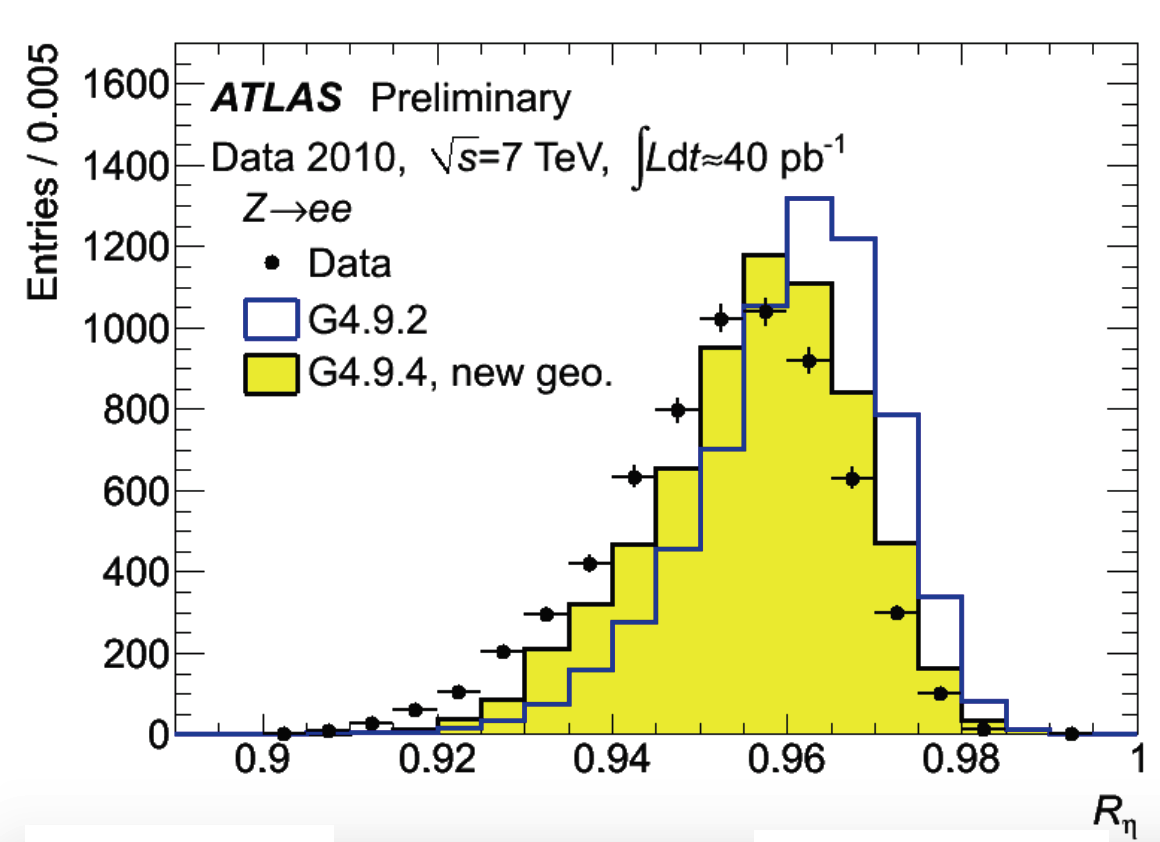
\includegraphics[width=12cm]{G4.png}\\
\end{frame}
%------------------------------------------------

%------------------------------------------------
\begin{frame}
\frametitle{2D profile of the cluster in the 2nd layer, 7x11 cells }

\centering
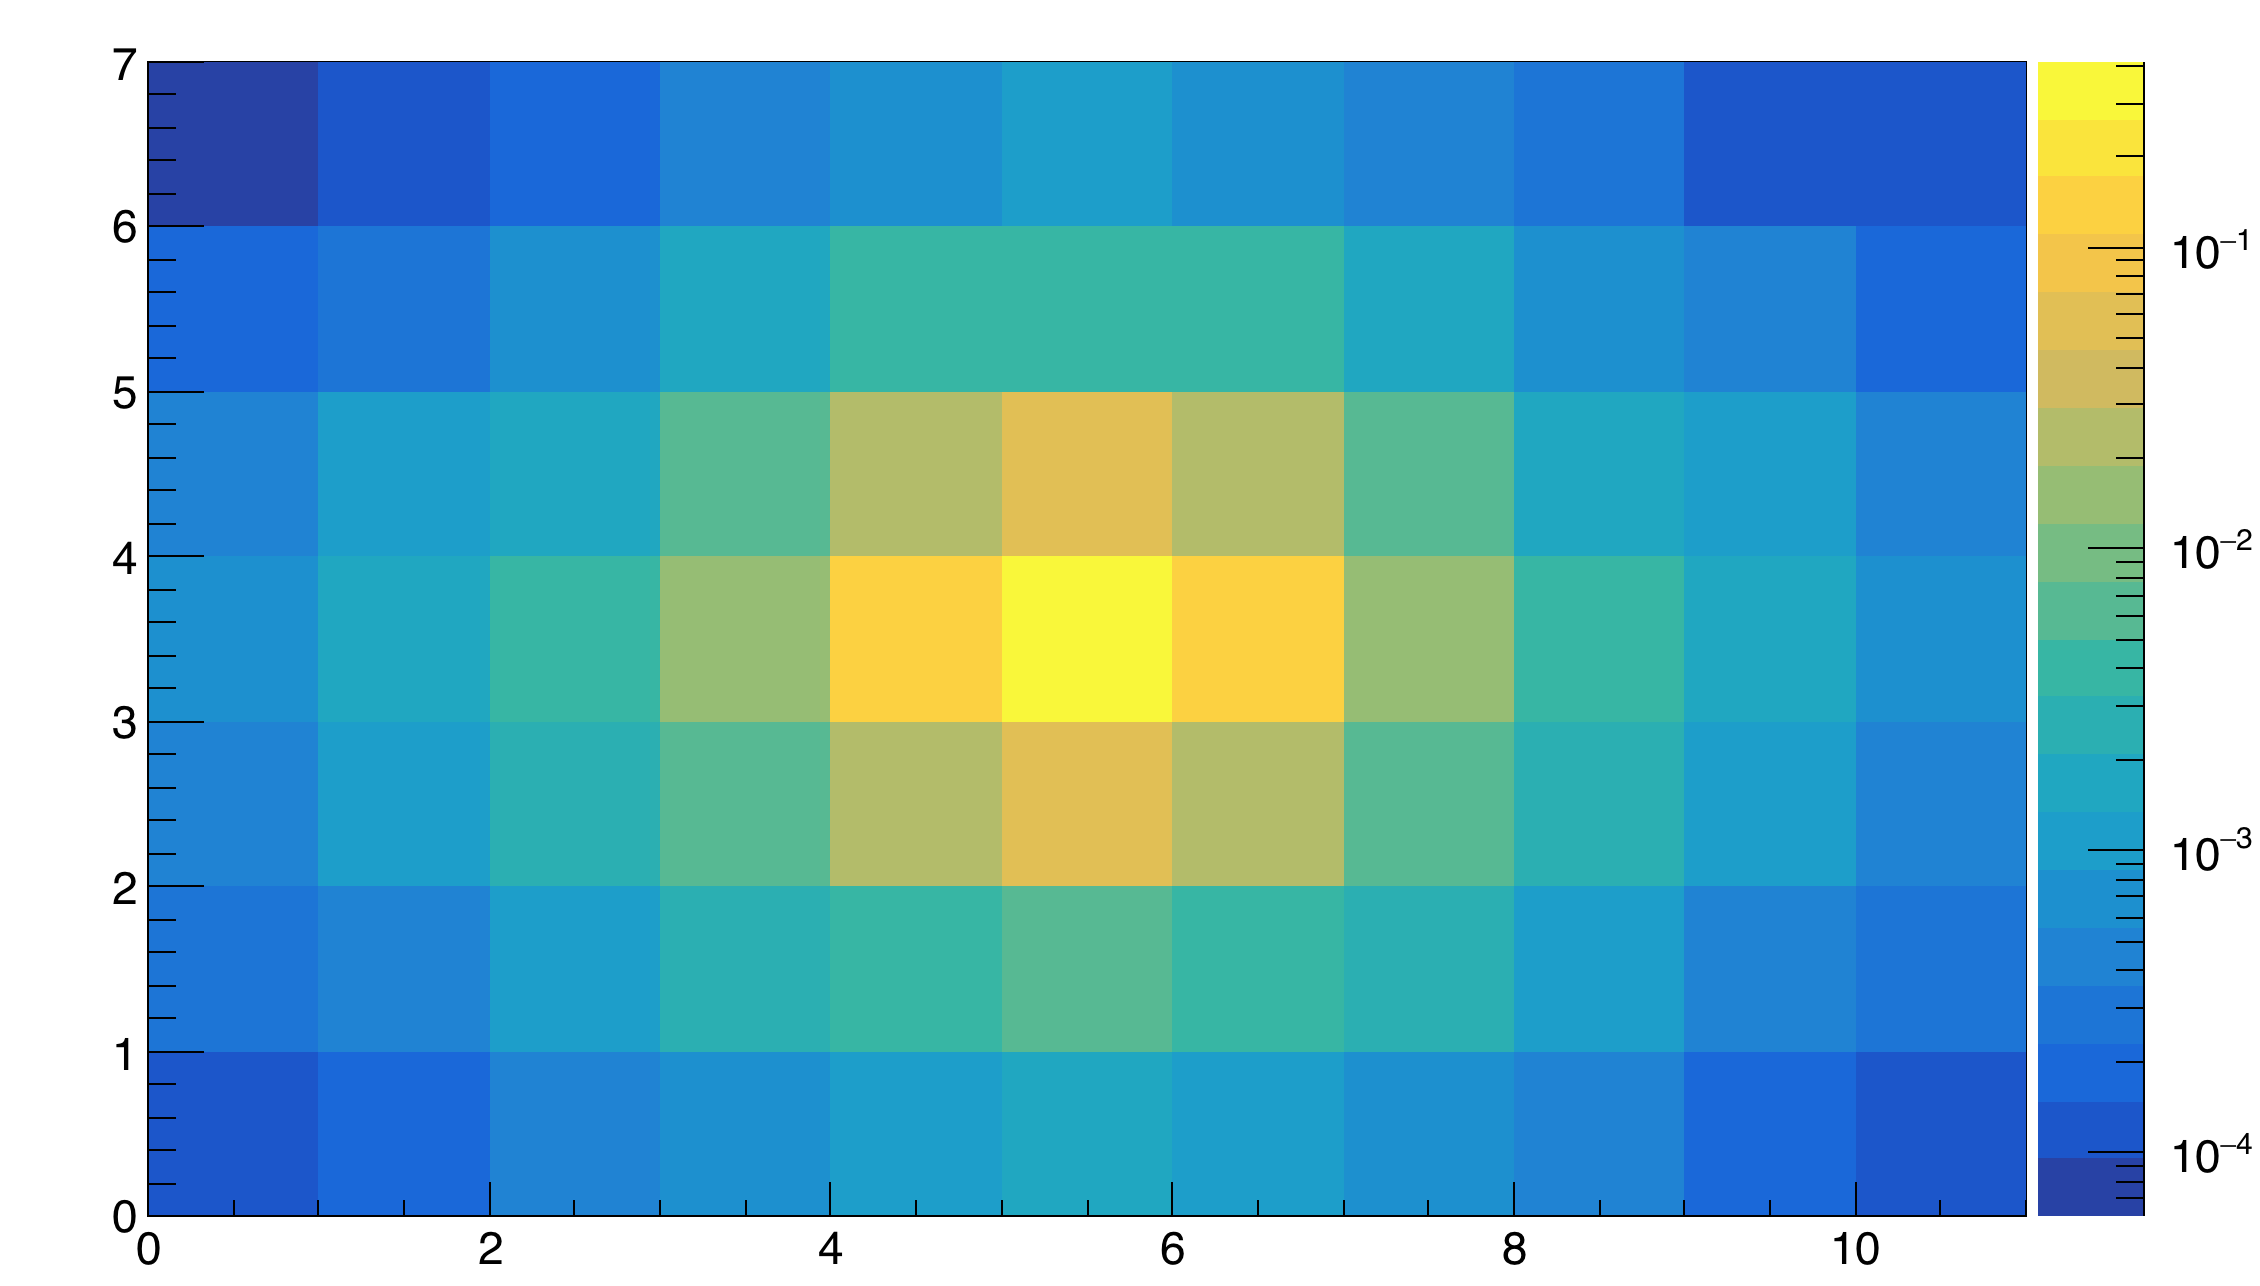
\includegraphics[height=3cm]{logscale.png}\\

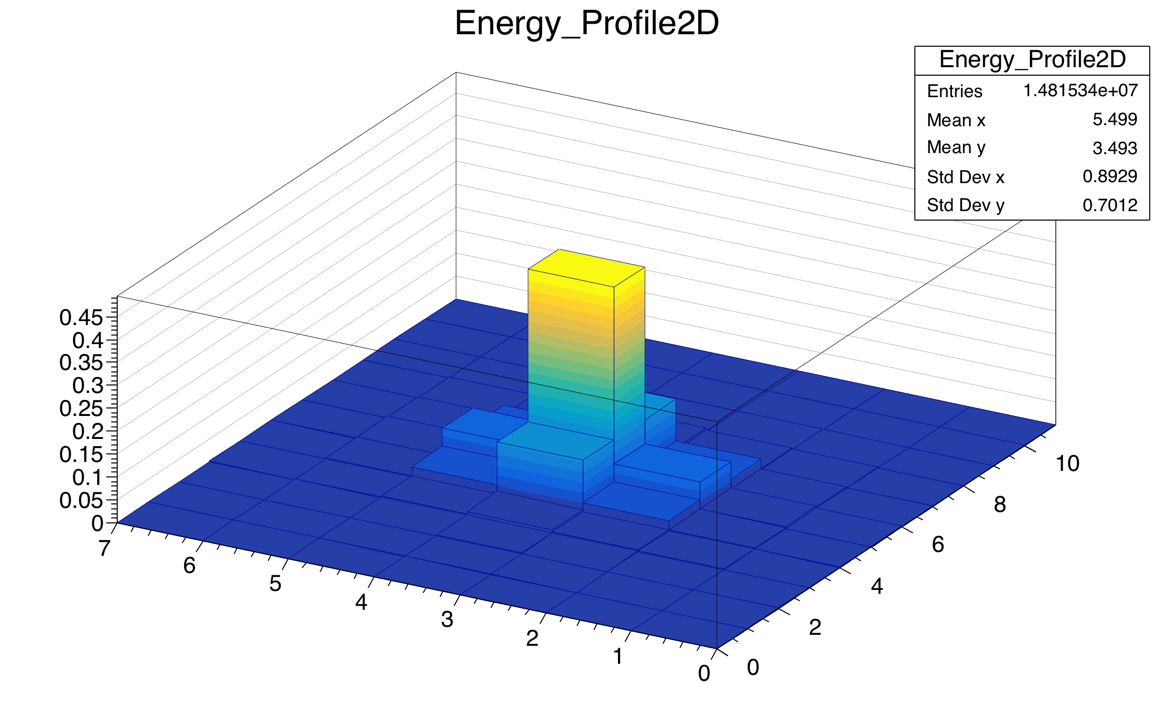
\includegraphics[height=5cm]{2dProfile.png}\\

\end{frame}
%------------------------------------------------

%------------------------------------------------
\begin{frame}
\frametitle{Shower shapes: 2nd layer variables}

\begin{itemize}
\item Lateral shower width $W_{\eta^2} = \sqrt{\sum(E_i \eta^{2}_{i})-(\sum(E_i \eta_{i})/\sum(E_i))^2}$ calculated within a window of 3x5 cells
\item $R_{\phi}$ - ratio of the energy in 3x3 cells over the energy in 3x7 cells centered at the electron cluster position.
\item $R_{\eta}$ - ratio of the energy in 3x7 cells over the energy in 7x7 cells centered at the electron cluster position.

\end{itemize}
\begin{columns}[t]
\column{.5\textwidth}
\centering
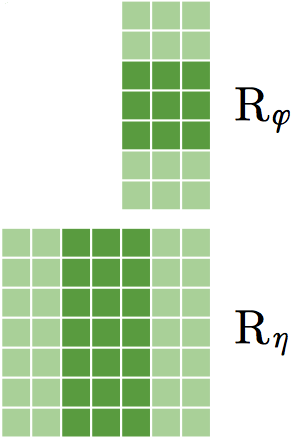
\includegraphics[width=4cm,height=5cm]{reta_rphi.png}\\

\column{.5\textwidth}
\centering
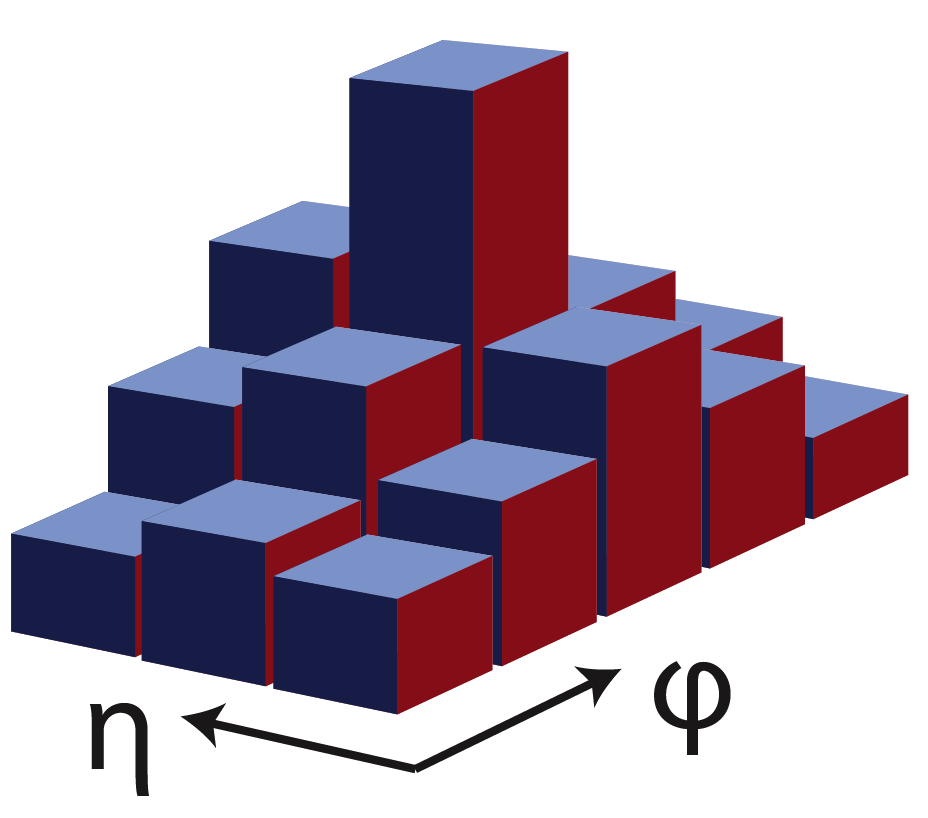
\includegraphics[width=6cm,height=5cm]{Weta2.png}\\
\end{columns}
\centering

\end{frame}
%------------------------------------------------
%------------------------------------------------
\begin{frame}
\frametitle{Energy profile in $\eta$ and $R_\eta$, $\eta \in (0.4, 0.6)$ }

\begin{columns}[t]
\column{.5\textwidth}
\centering
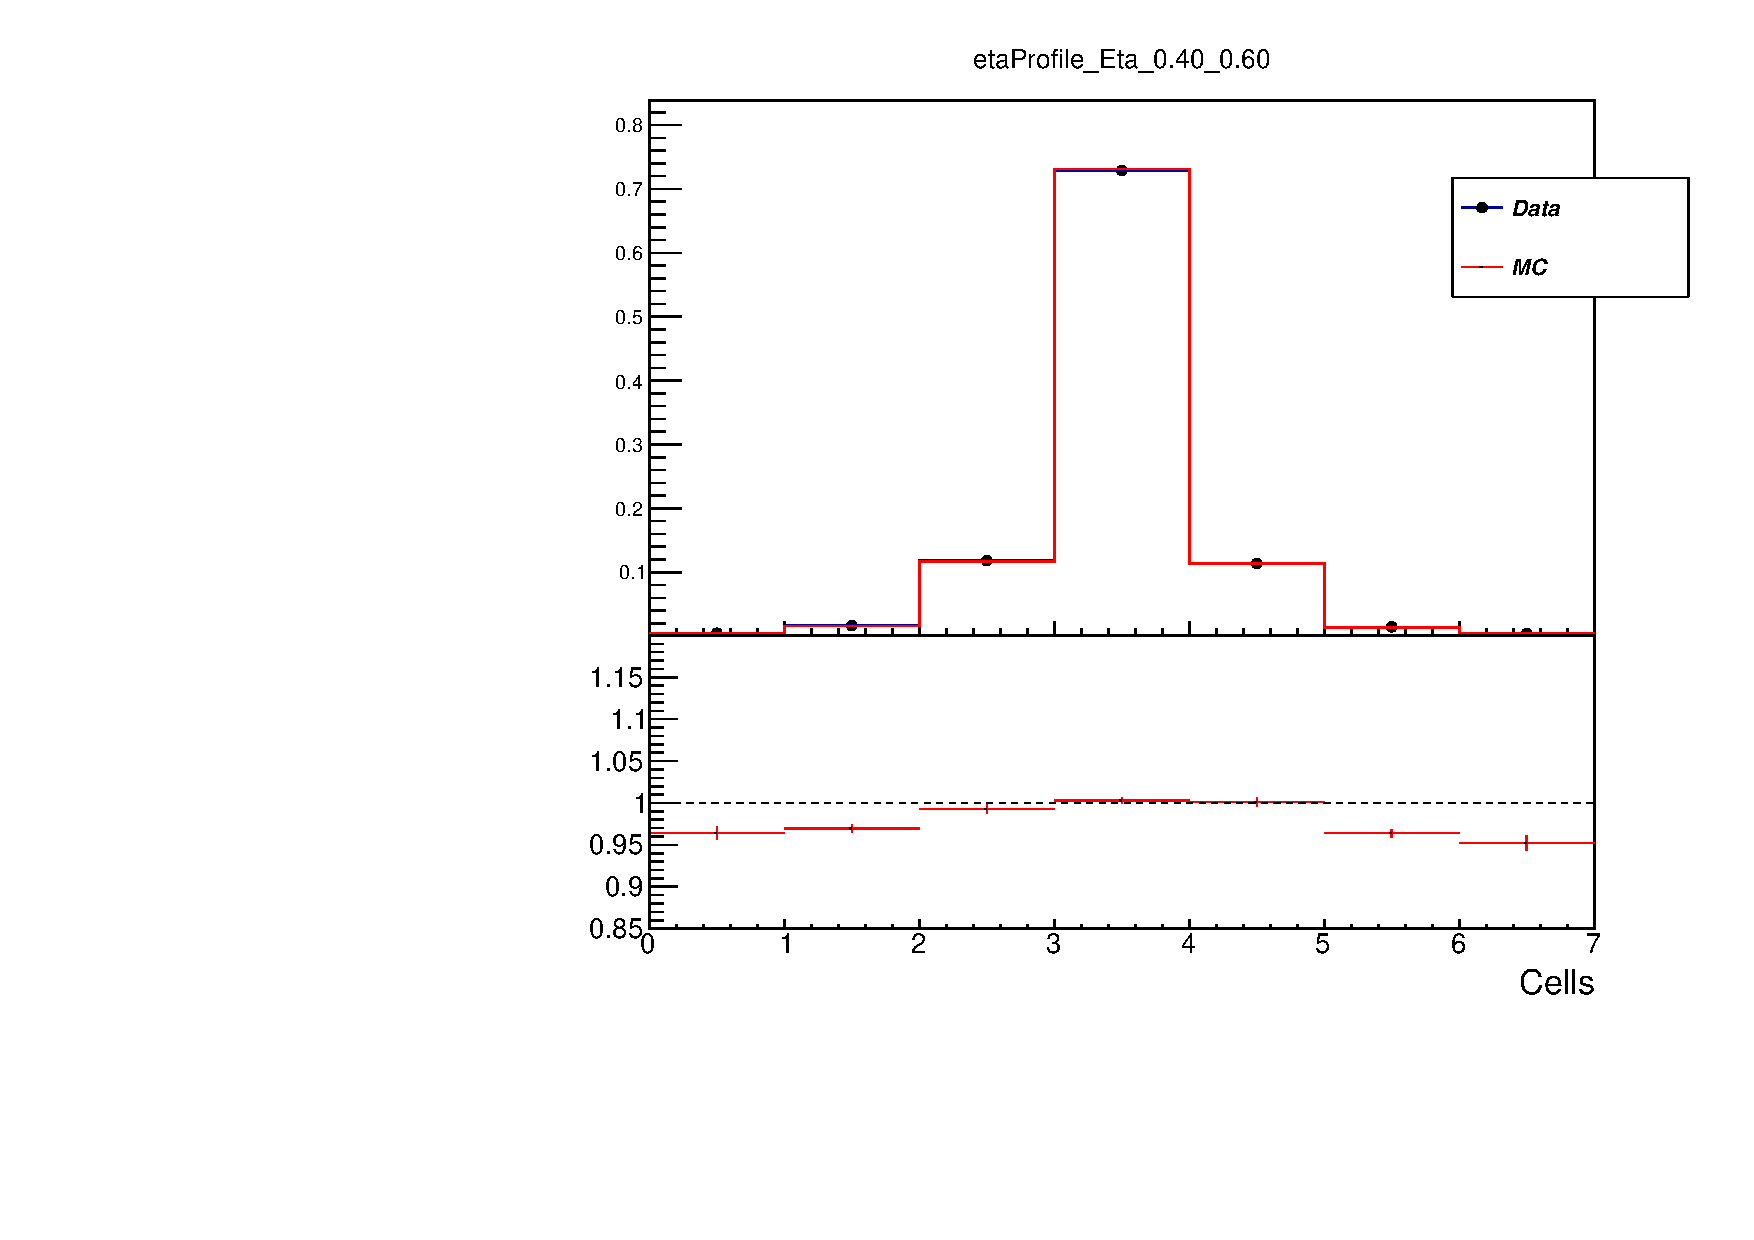
\includegraphics[width=6cm]{etaProfile2_Eta_4_6.pdf}\\
\column{.5\textwidth}
\centering
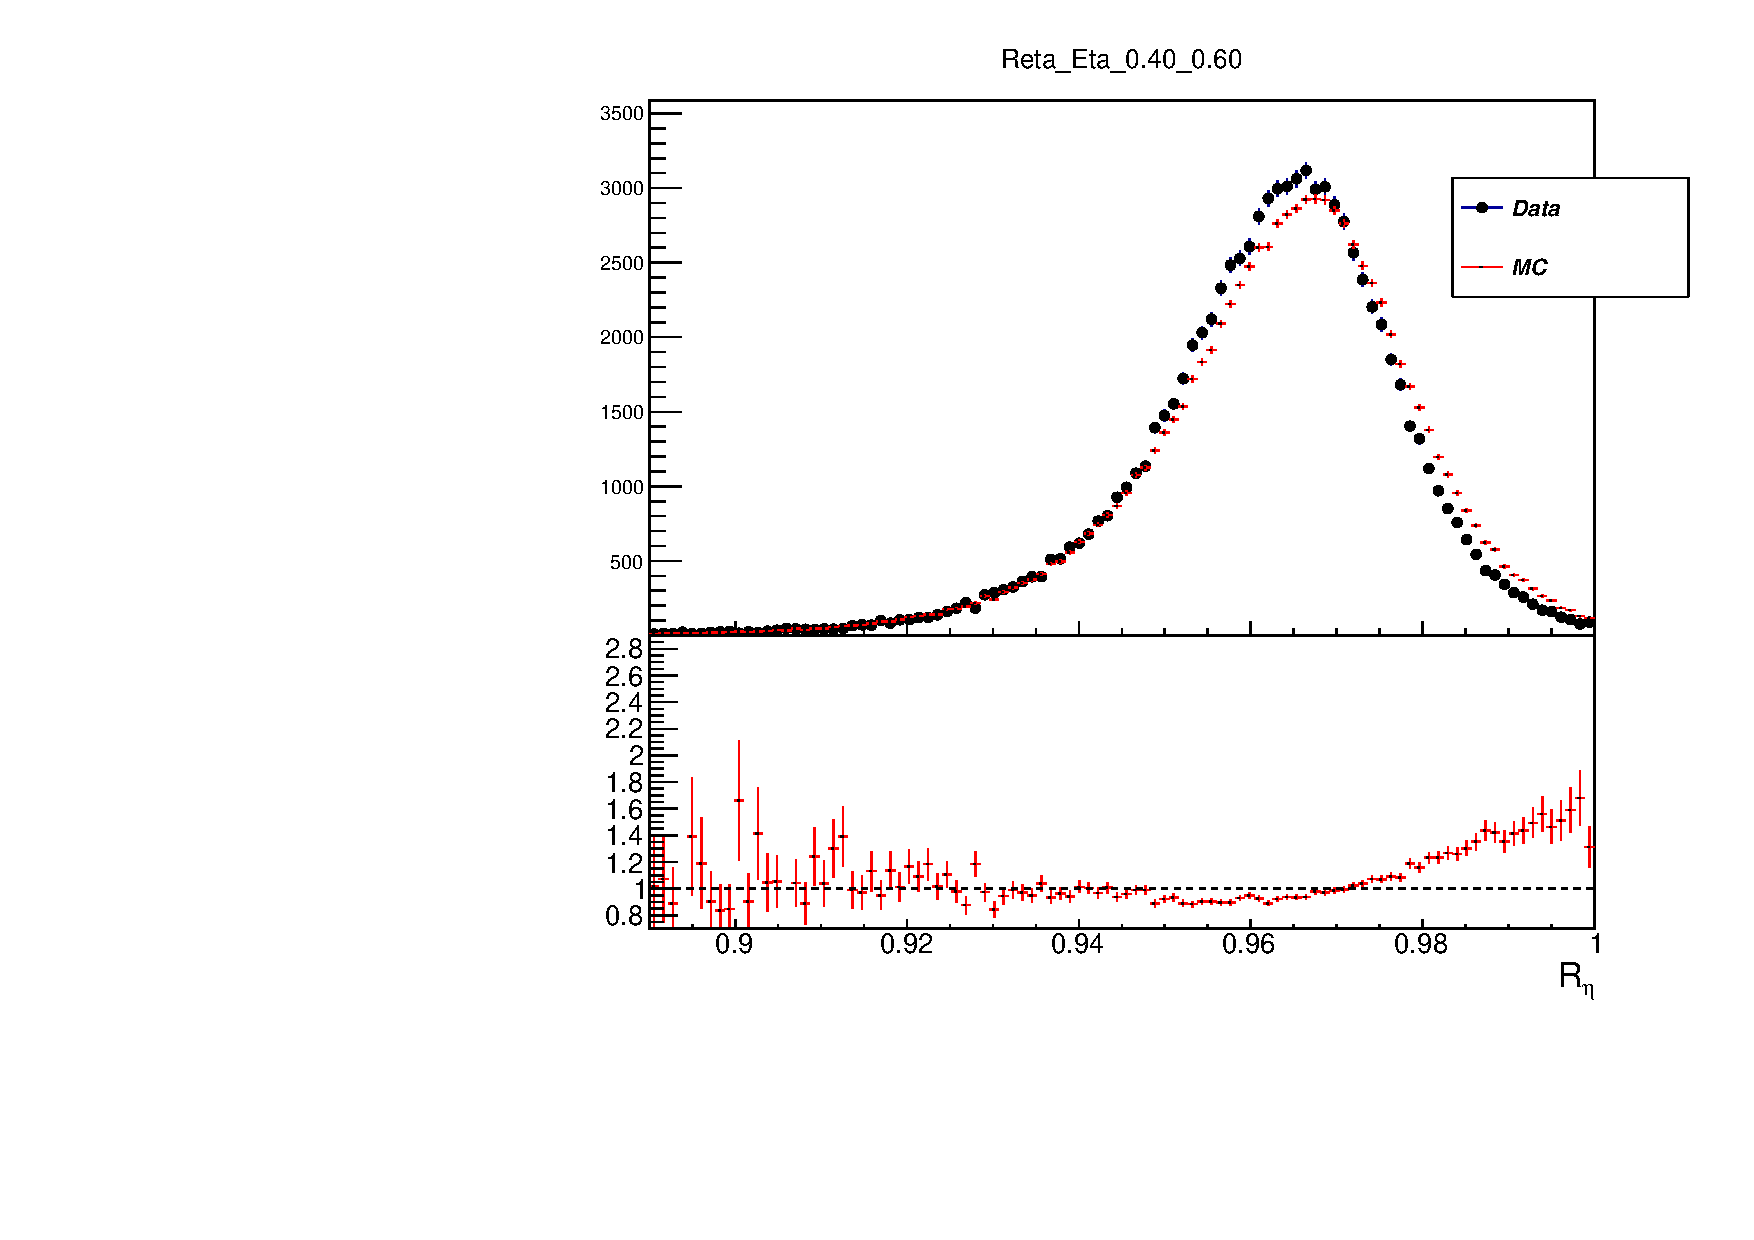
\includegraphics[width=6cm]{Reta2_Eta_4_6.pdf}\\

\end{columns}
\end{frame}
%------------------------------------------------
%------------------------------------------------
\begin{frame}
\frametitle{Energy profile in $\eta$ and $R_\eta$, $\eta \in (1.8, 2.0)$}

\begin{columns}[t]
\column{.5\textwidth}
\centering
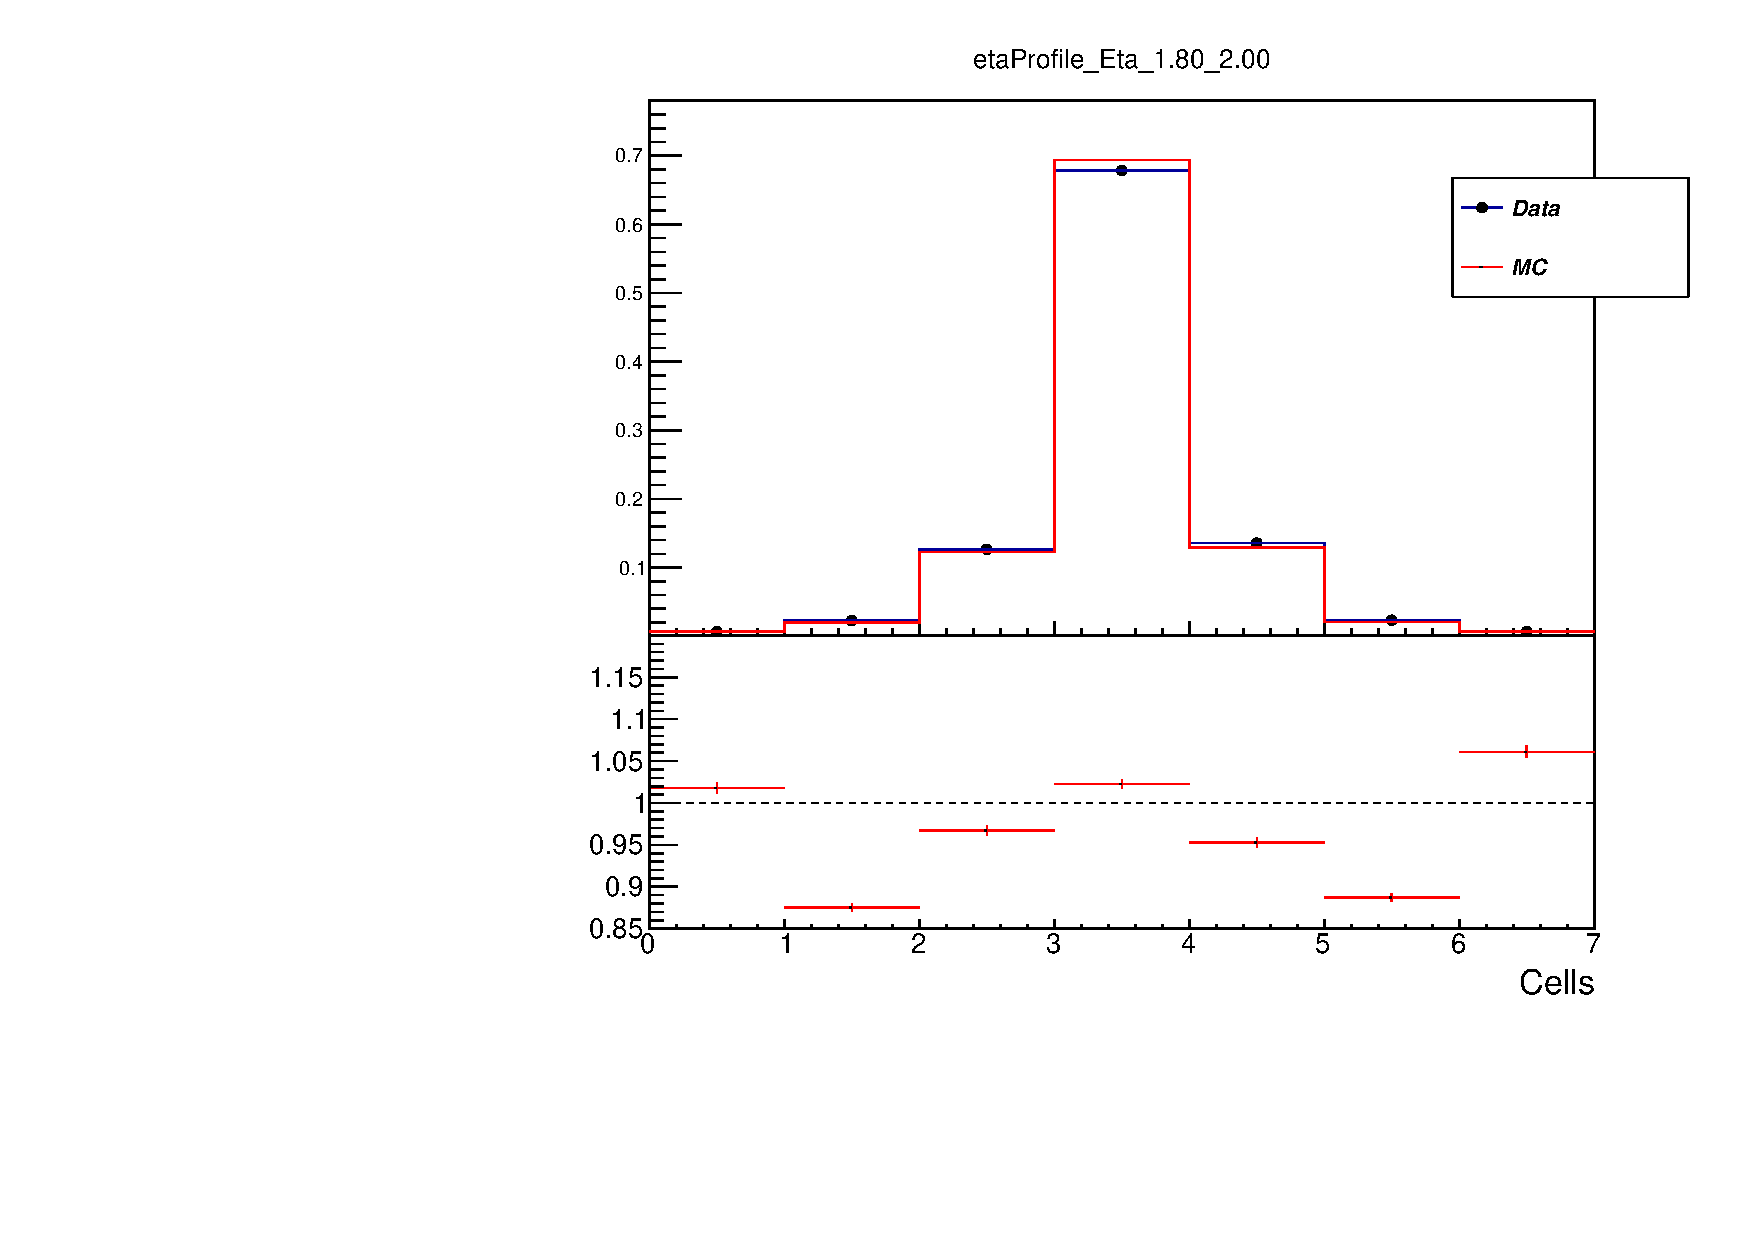
\includegraphics[width=6cm]{etaProfile2_Eta_18_20.pdf}
\column{.5\textwidth}
\centering
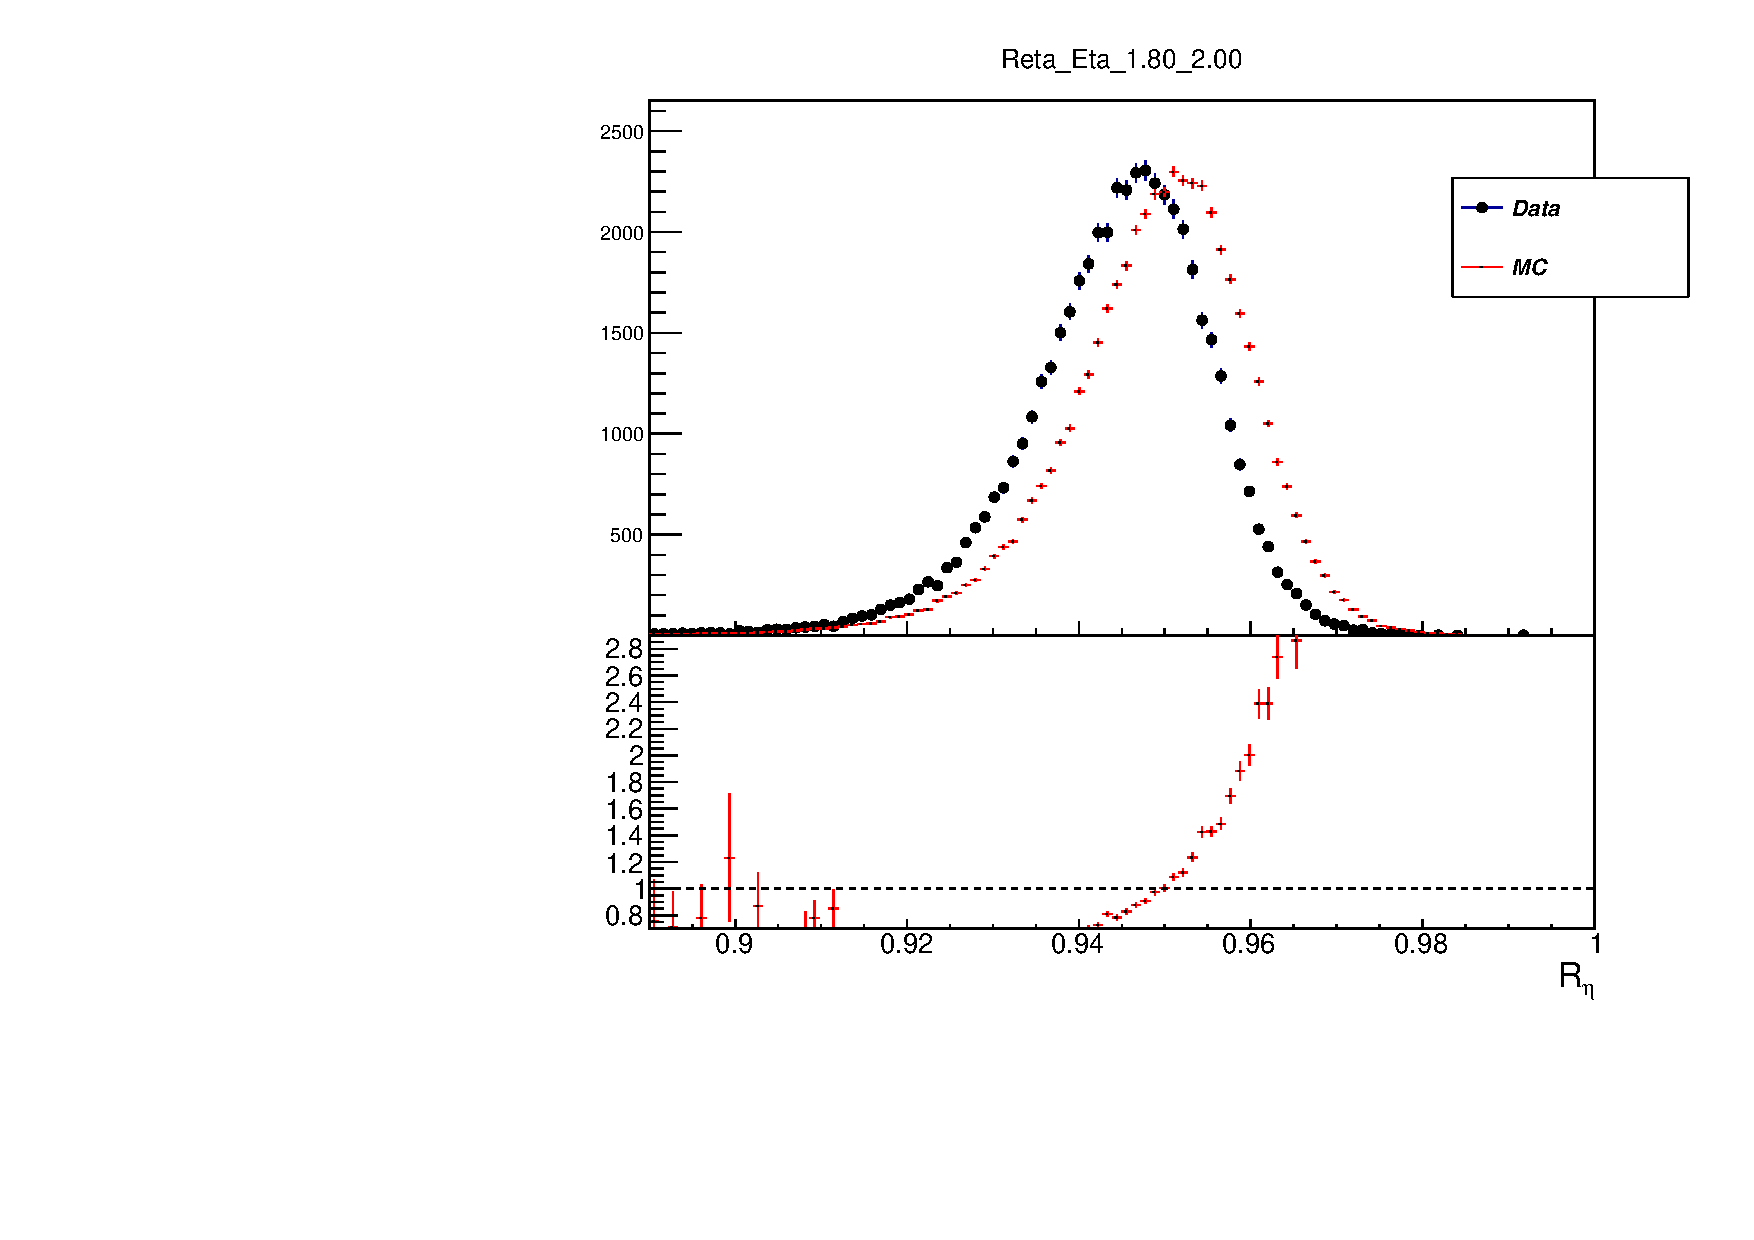
\includegraphics[width=6cm]{Reta2_Eta_18_20.pdf}
\end{columns}
\end{frame}
%------------------------------------------------
%------------------------------------------------
\begin{frame}
\frametitle{Shower shapes:$W_{\eta^2}$, $\eta \in (0.4, 0.6)$ and \textbf{$(1.8, 2.0)$}}

\begin{columns}[t]
\column{.5\textwidth}
\centering
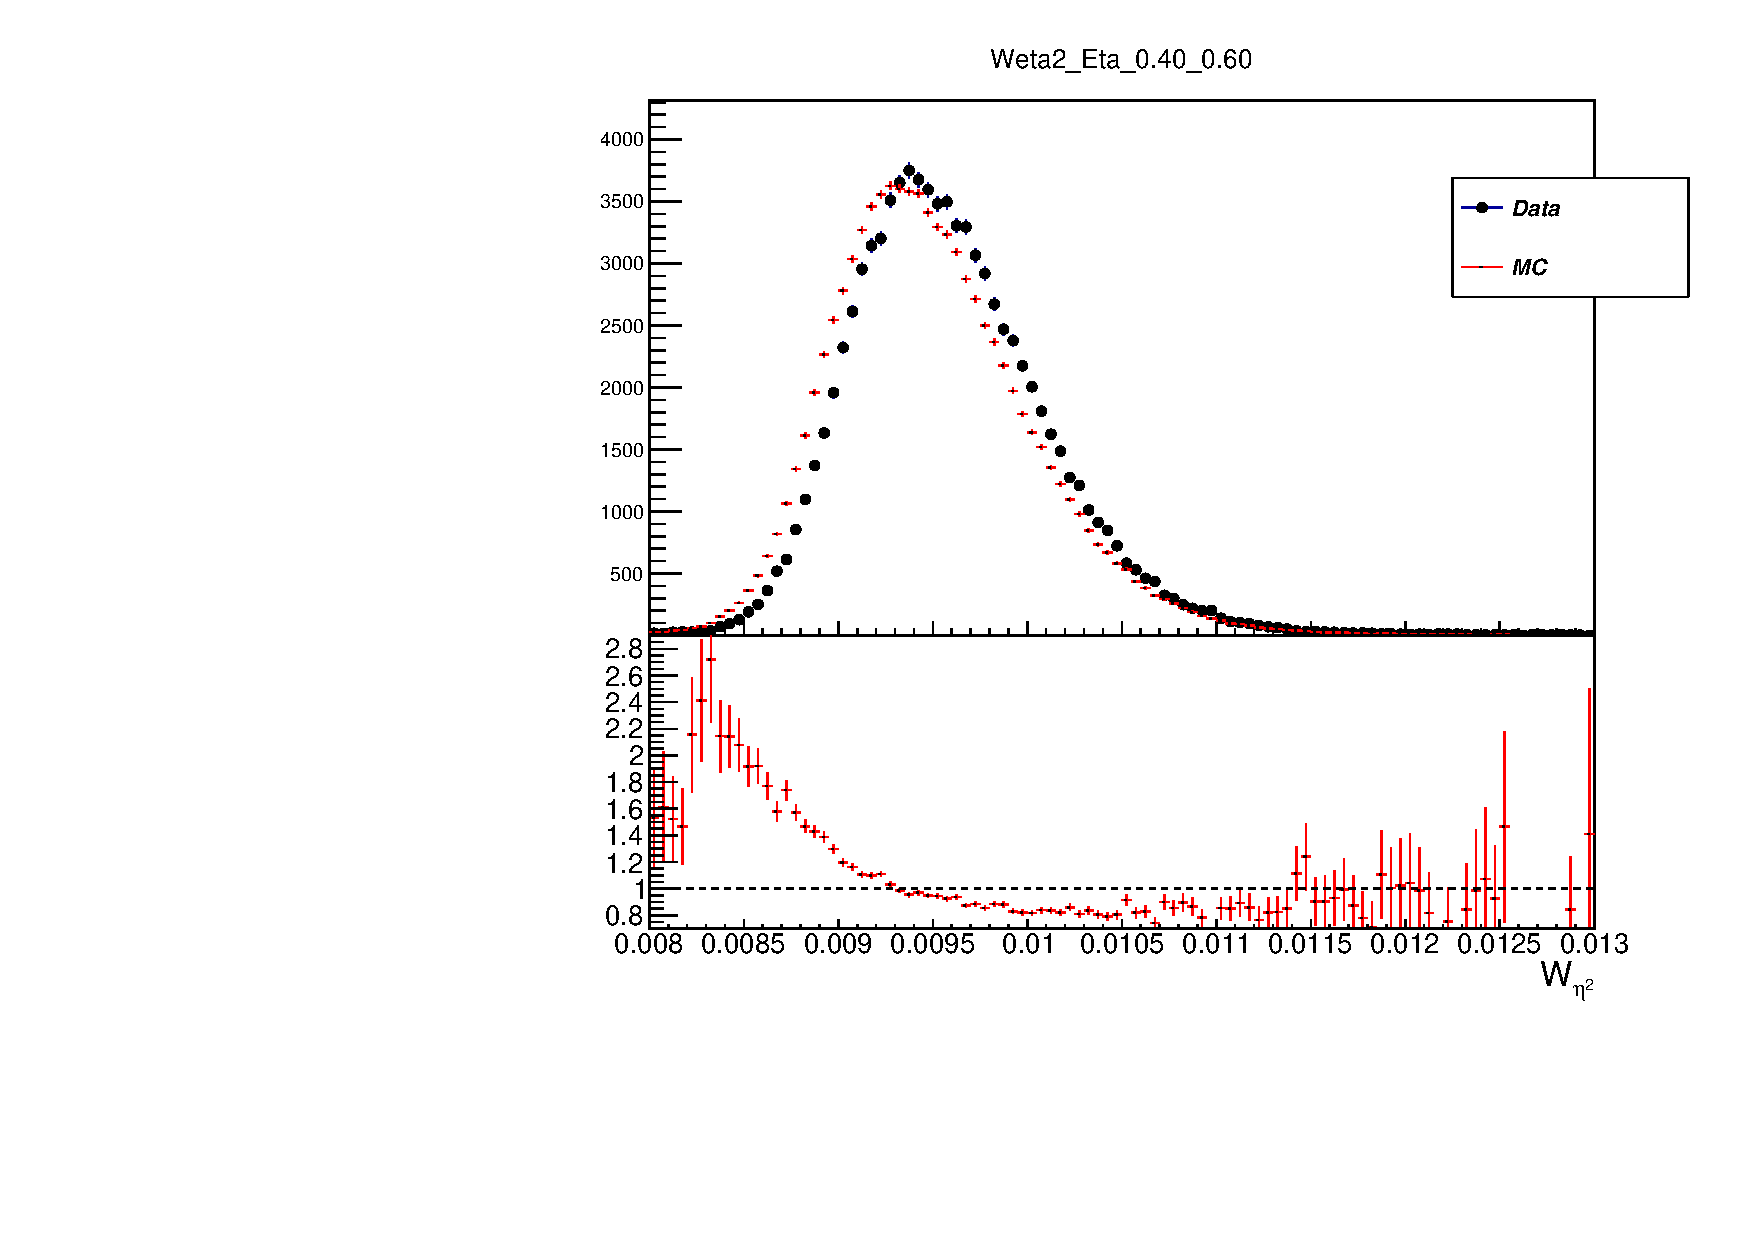
\includegraphics[width=6cm]{weta22_Eta_4_6.pdf}\\
\column{.5\textwidth}
\centering
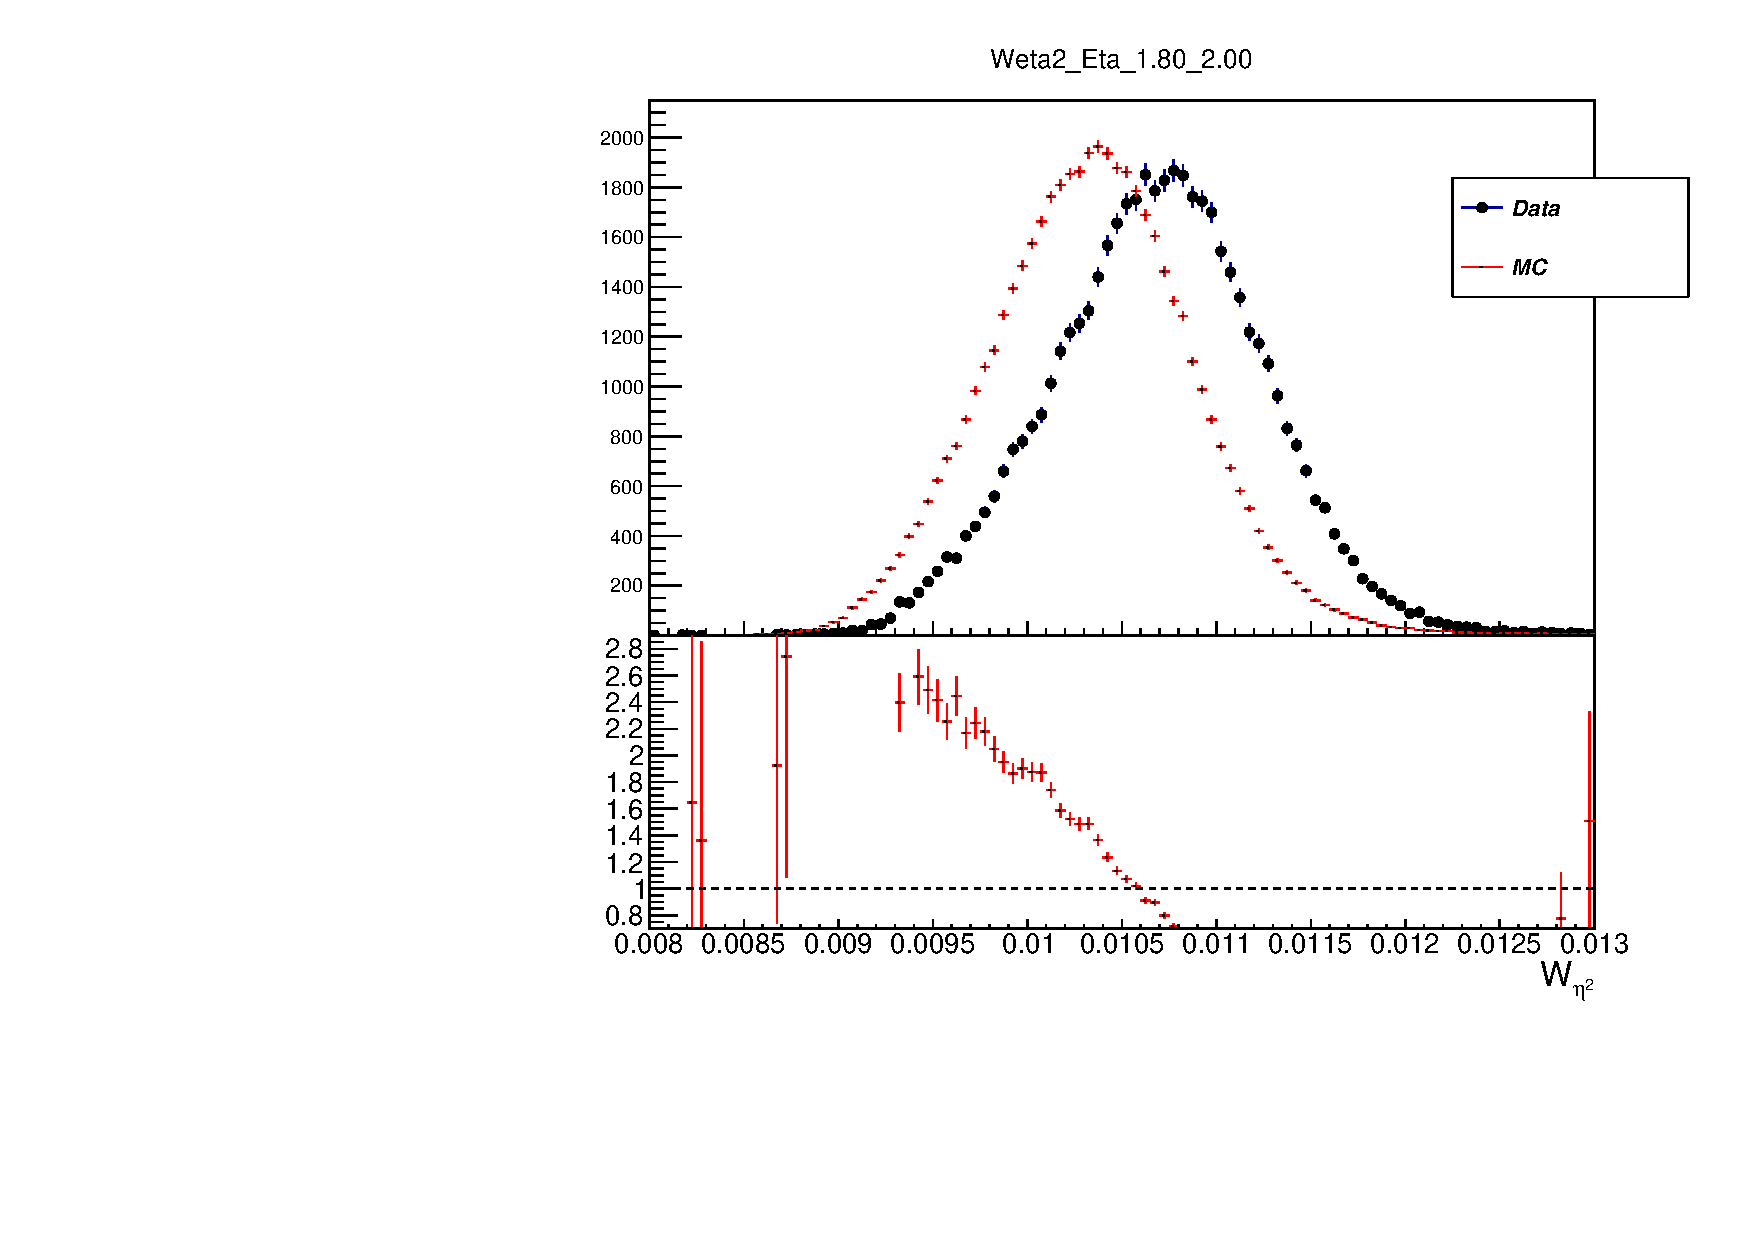
\includegraphics[width=6cm]{weta22_Eta_18_20.pdf}\\
\end{columns}
\end{frame}
%------------------------------------------------
%------------------------------------------------
\begin{frame}
\frametitle{Energy profile in $\phi$ and $R_\phi$, $\eta \in (0.4, 0.6)$ }

\begin{columns}[t]
\column{.5\textwidth}
\centering
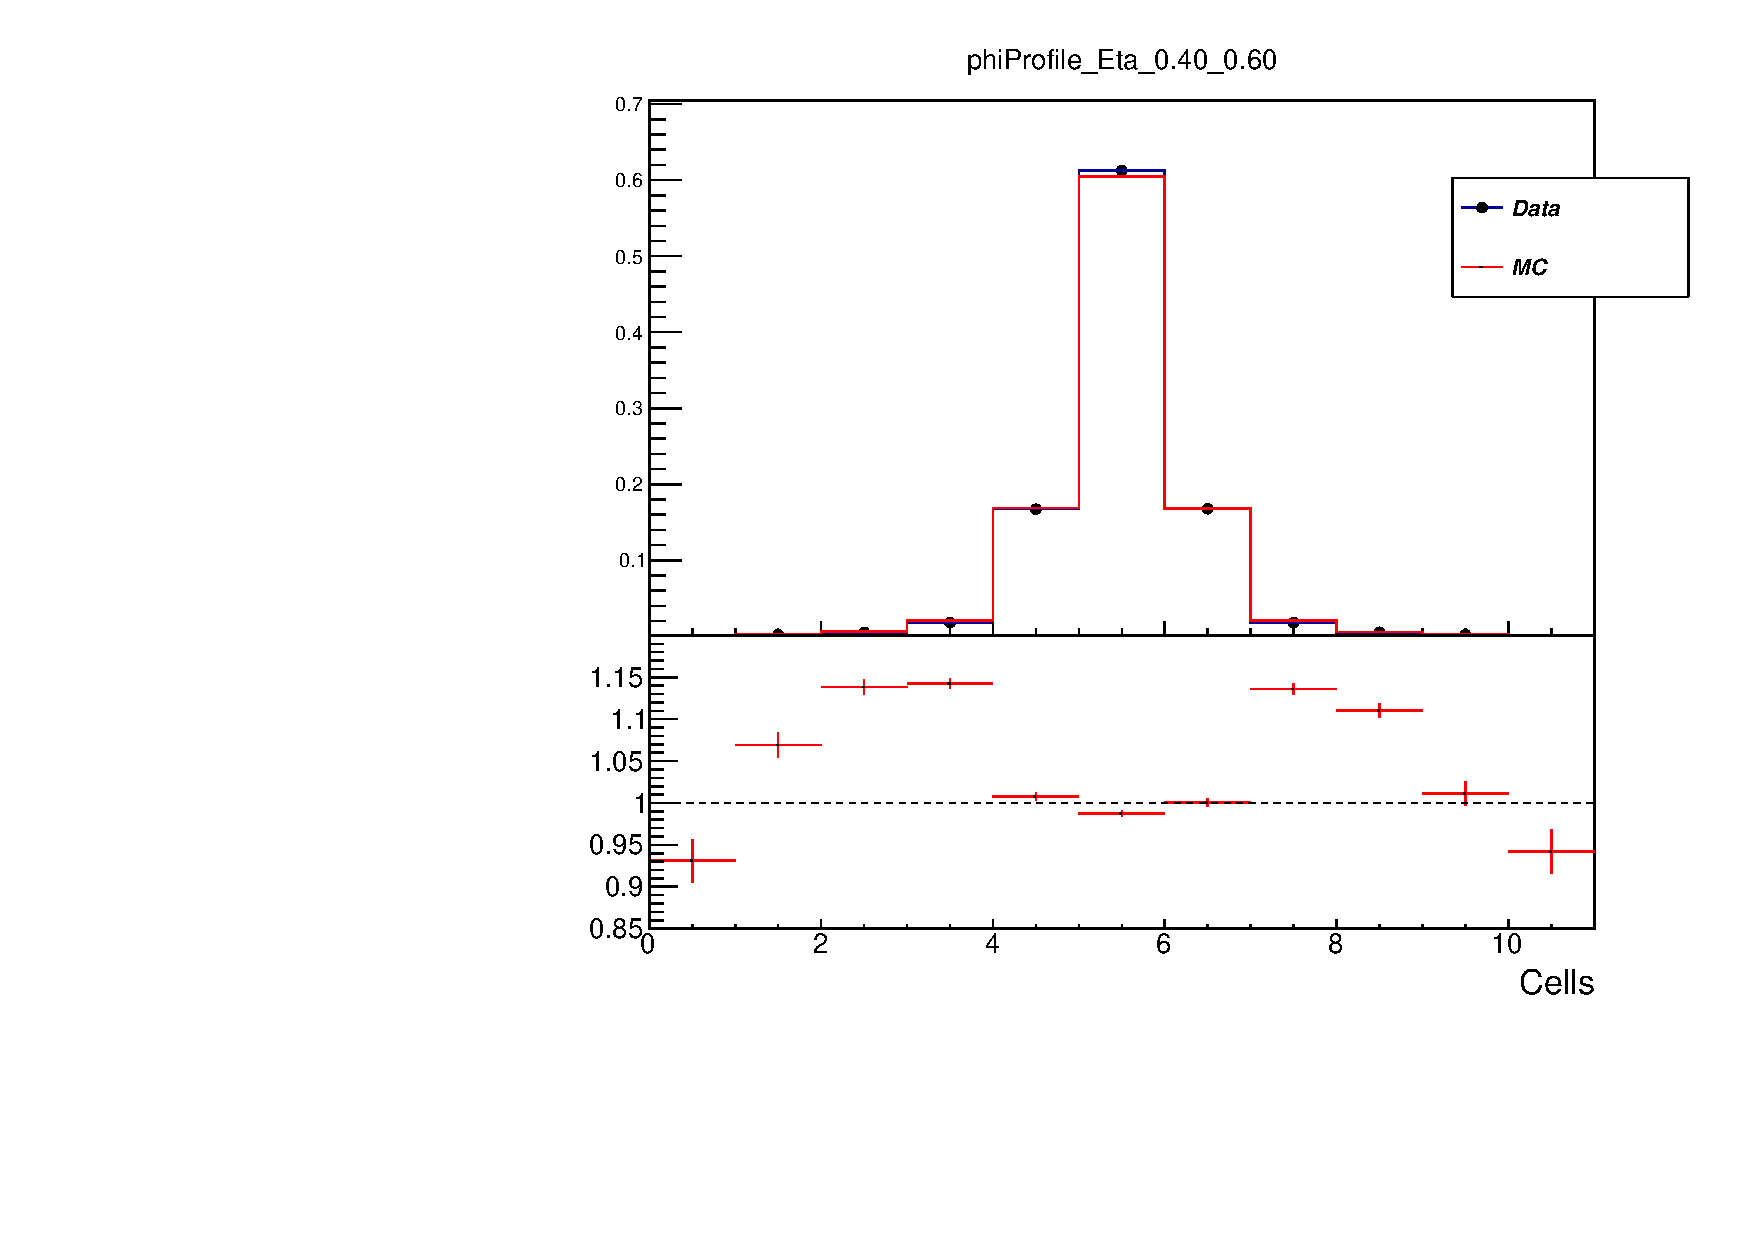
\includegraphics[width=6cm]{phiProfile2_Eta_4_6.pdf}\\
\column{.5\textwidth}
\centering
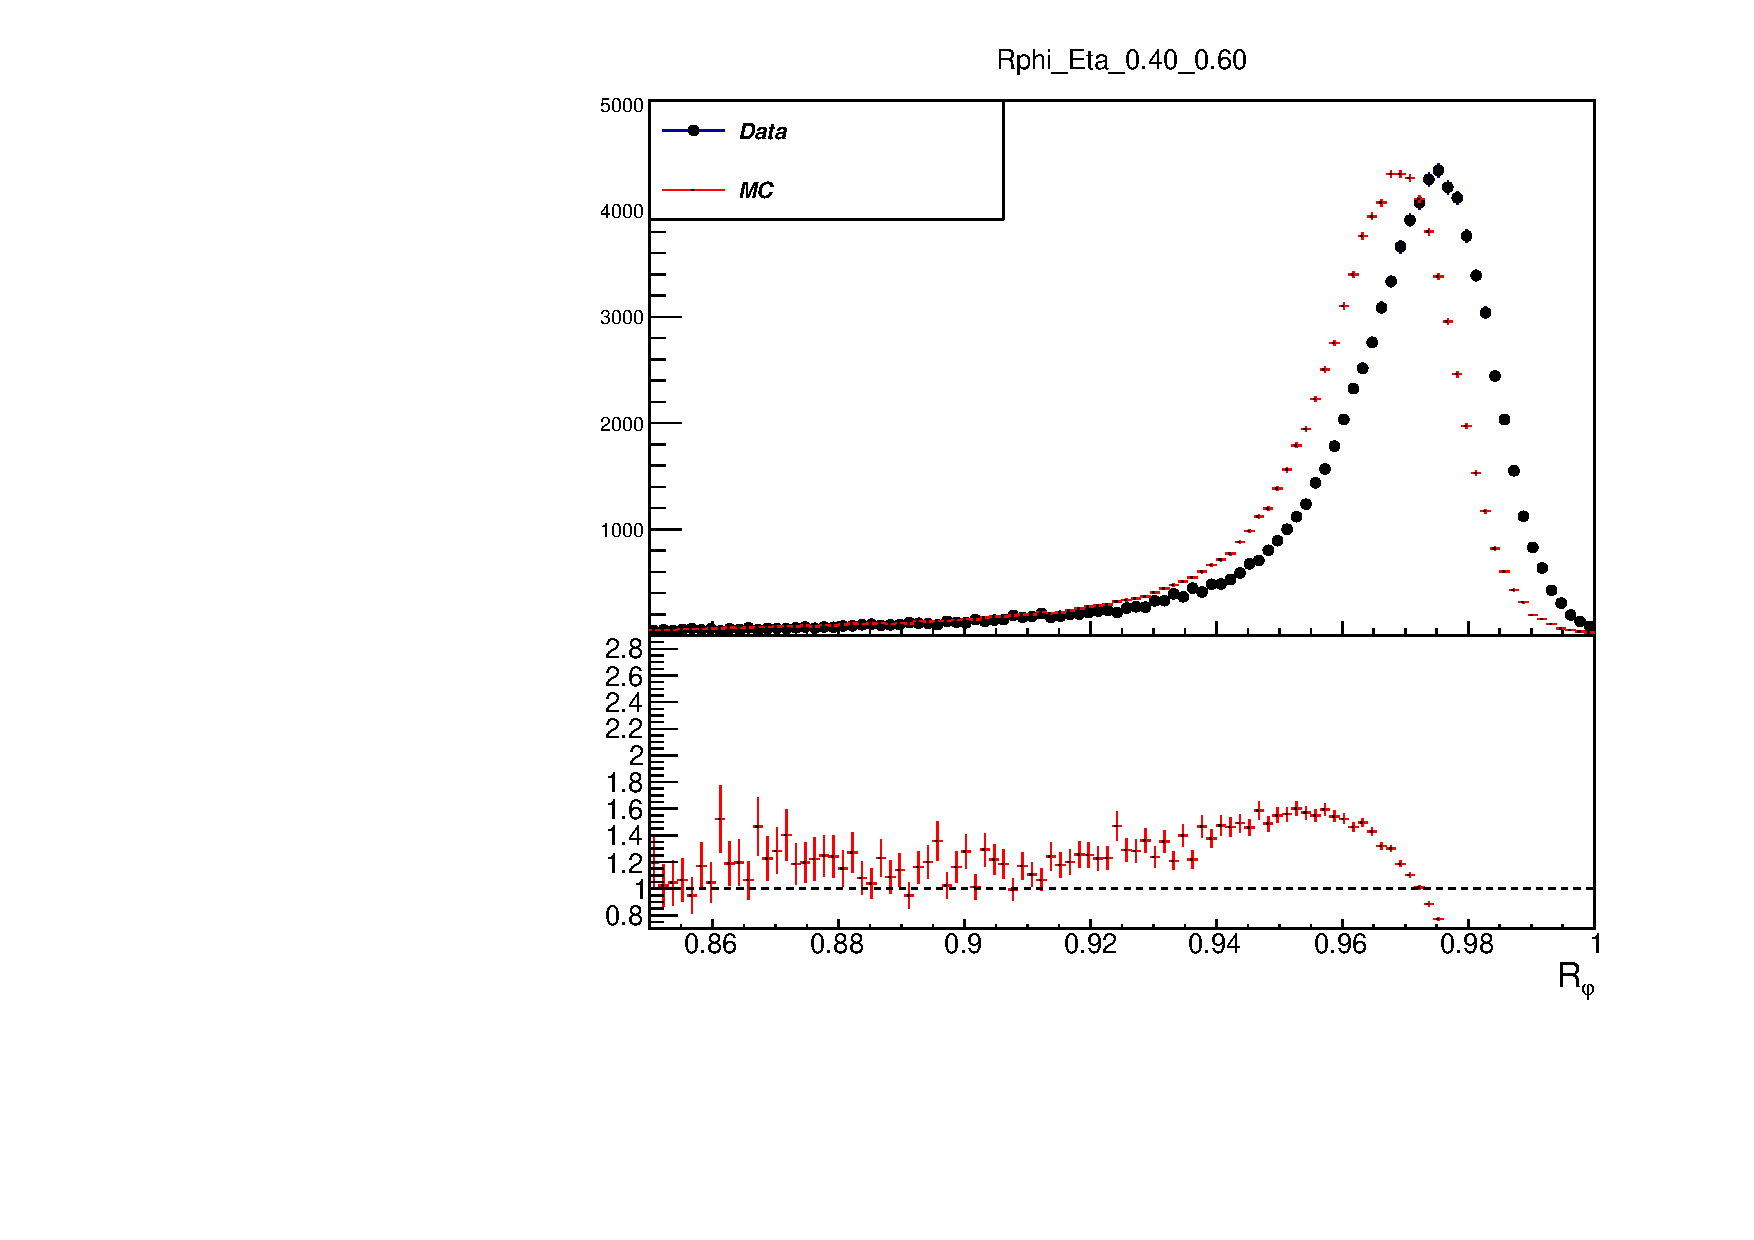
\includegraphics[width=6cm]{Rphi2_Eta_4_6.pdf}\\

\end{columns}
\end{frame}
%------------------------------------------------

%------------------------------------------------
\begin{frame}
\frametitle{Energy profile in $\phi$ and $R_\phi$,  $\eta \in (1.8, 2.0)$}

\begin{columns}[t]
\column{.5\textwidth}
\centering
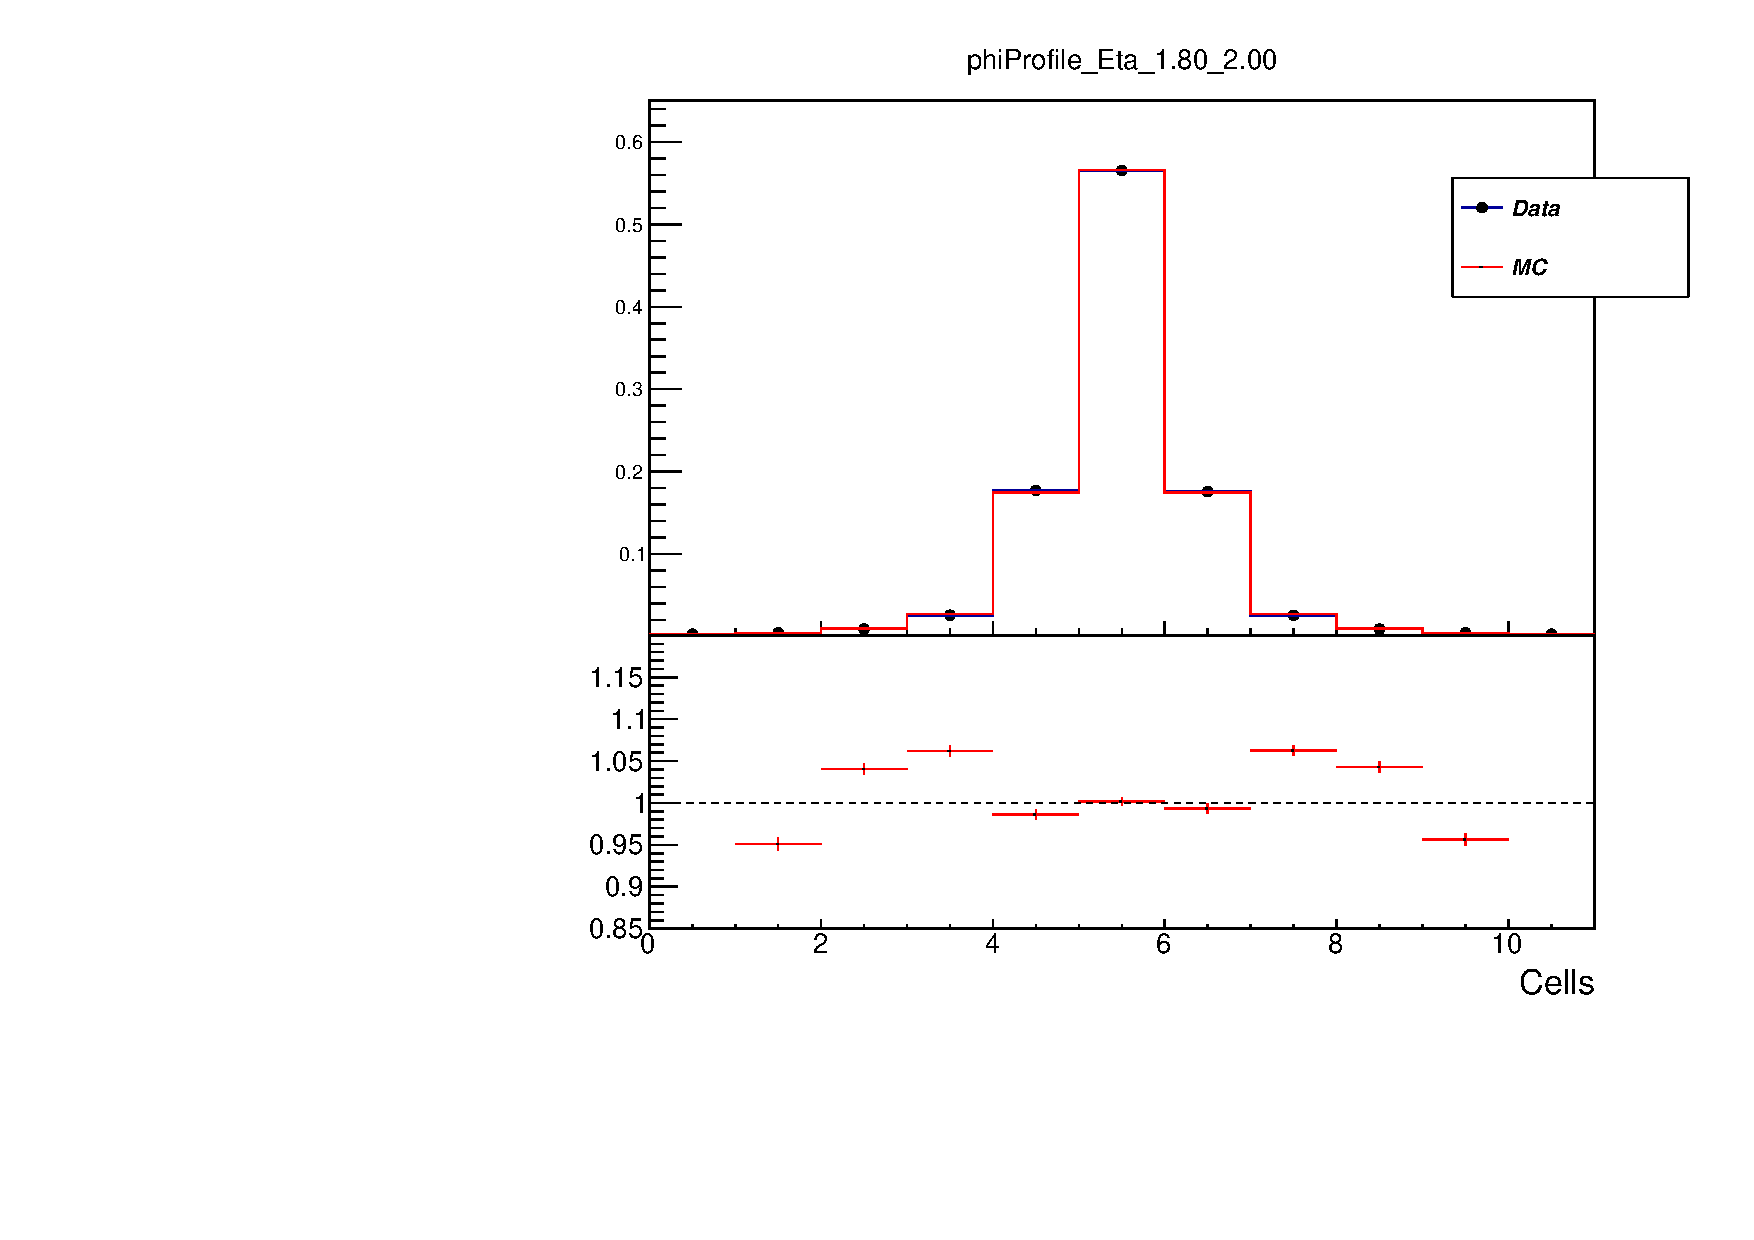
\includegraphics[width=6cm]{phiProfile2_Eta_18_20.pdf}
\column{.5\textwidth}
\centering
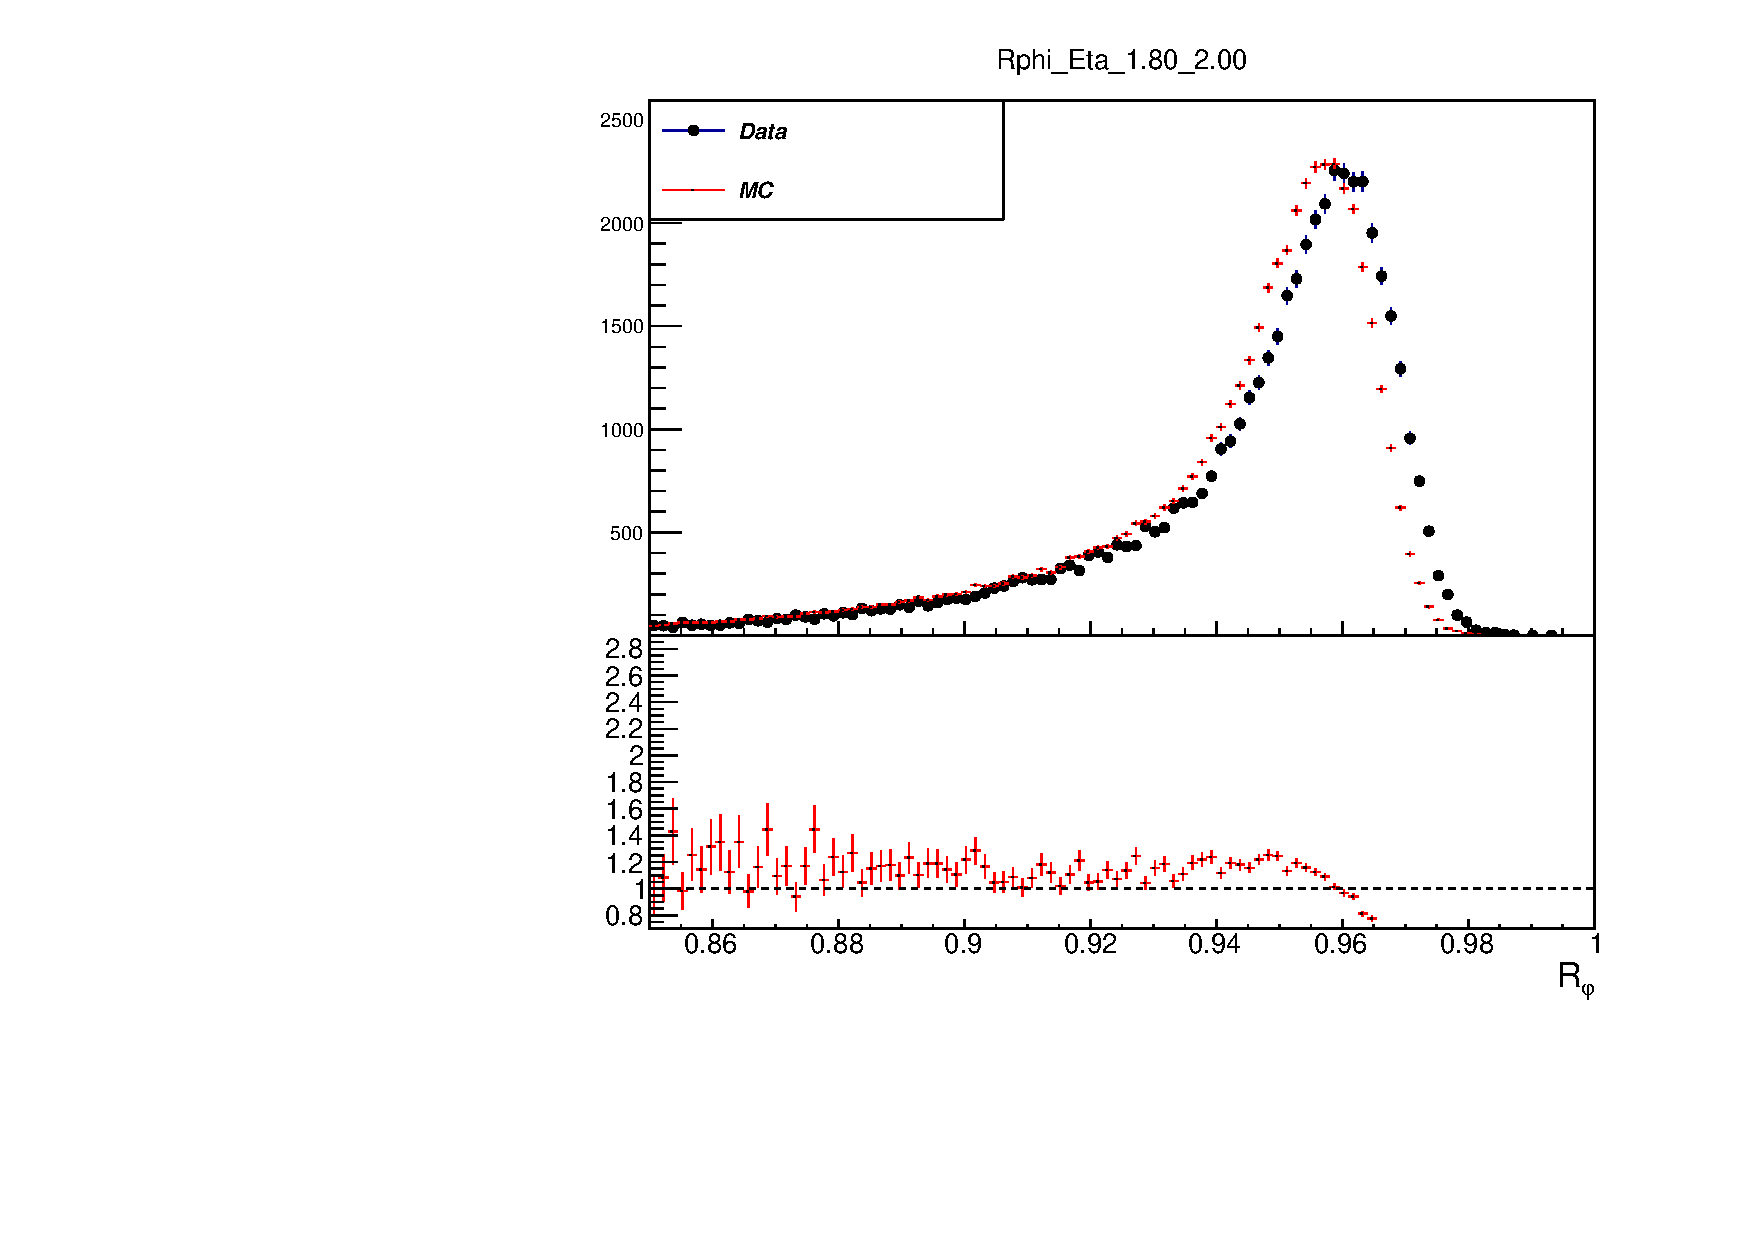
\includegraphics[width=6cm]{Rphi2_Eta_18_20.pdf}
\end{columns}
\end{frame}
%------------------------------------------------


%------------------------------------------------
\begin{frame}
\frametitle{Energy profiling conclusions}
\begin{itemize}
\item The shower shapes are $\eta$-dependent, so 14 slices in $\eta$ were considered in the range of  $\textbar \eta\textbar = 0 - 2.4$
\item The barrel $\textbar \eta\textbar = 0 - 1.37$ and the endcap $\textbar \eta\textbar = 1.52 - 2.4$ regions demonstrate different behavior.
\item The data is wider in $\eta$ and narrower $\phi$ than the MC-modelled shower.
\item The discrepancy is higher in the barrel for $\phi$ profile and in the endcap for $\eta$.
\item This discrepancy reflects two factors: the influence of the magnetic field and  differences in solid material. 
\end{itemize}
\end{frame}
%------------------------------------------------

%------------------------------------------------
\begin{frame}
\frametitle{Reweighting procedure}
Reweighting is performed in two steps: 
\begin{itemize}
\item Calculation of the 2D correction matrix containing cluster cell corrections for each $\eta$ slice 
\begin{equation}
\nonumber
   \large {M_{i}^{Correction} = \frac{E_{i}^{Data}}{\Sigma E^{Data}} - \frac{E_{i}^{MC}}{\Sigma E^{MC}}}
\end{equation}
$\Sigma_i M_i^{Correction} = 0$, $i = 1..77$.\\
$E_i^{Data}$, $E_i^{MC}$ - matrix elements of the averaged energy profiles. 
\item Calculation of the reweighted energy for electron cluster cells in every MC event
\begin{equation}
\nonumber
   \large {E_{i}^{Reweighted} = {E_{i}^{Non-reweighted}(1+M_{i}^{Correction})}}
\end{equation}
\item Let's do a local test on the same set of MC events and see if it works.
\end{itemize}
\end{frame}

%------------------------------------------------
%------------------------------------------------

\begin{frame}
\frametitle{Event selection}

\begin{itemize}
\item Z->ee process considered (a modified EGAM1 derivation used)
\item 2 electrons, at least one has $p_T>25GeV$
\item  gradient isolation
\item  Tag and probe, no ID 
\item  Z invariant mass window 80 - 120 GeV 
\item  electron triggers: HLT\_e26\_lhtight\_nod0\_ivarloose, HLT\_e60\_lhmedium\_nod0, HLT\_e140\_lhloose\_nod0,HLT\_e300\_etcut
\item no pile-up reweighting
\item electrons must have a complete 7x11 cells cluster
\item Number of AOD-level events processed: \\
Data: 264786295 \\
MC: 79340000
\end{itemize}



\end{frame}
%------------------------------------------------


%------------------------------------------------
\begin{frame}
\frametitle{Reweighted energy profile in $\eta$ and $R_\eta$,  $\eta \in (0.4, 0.6)$}

\begin{columns}[t]
\column{.5\textwidth}
\centering
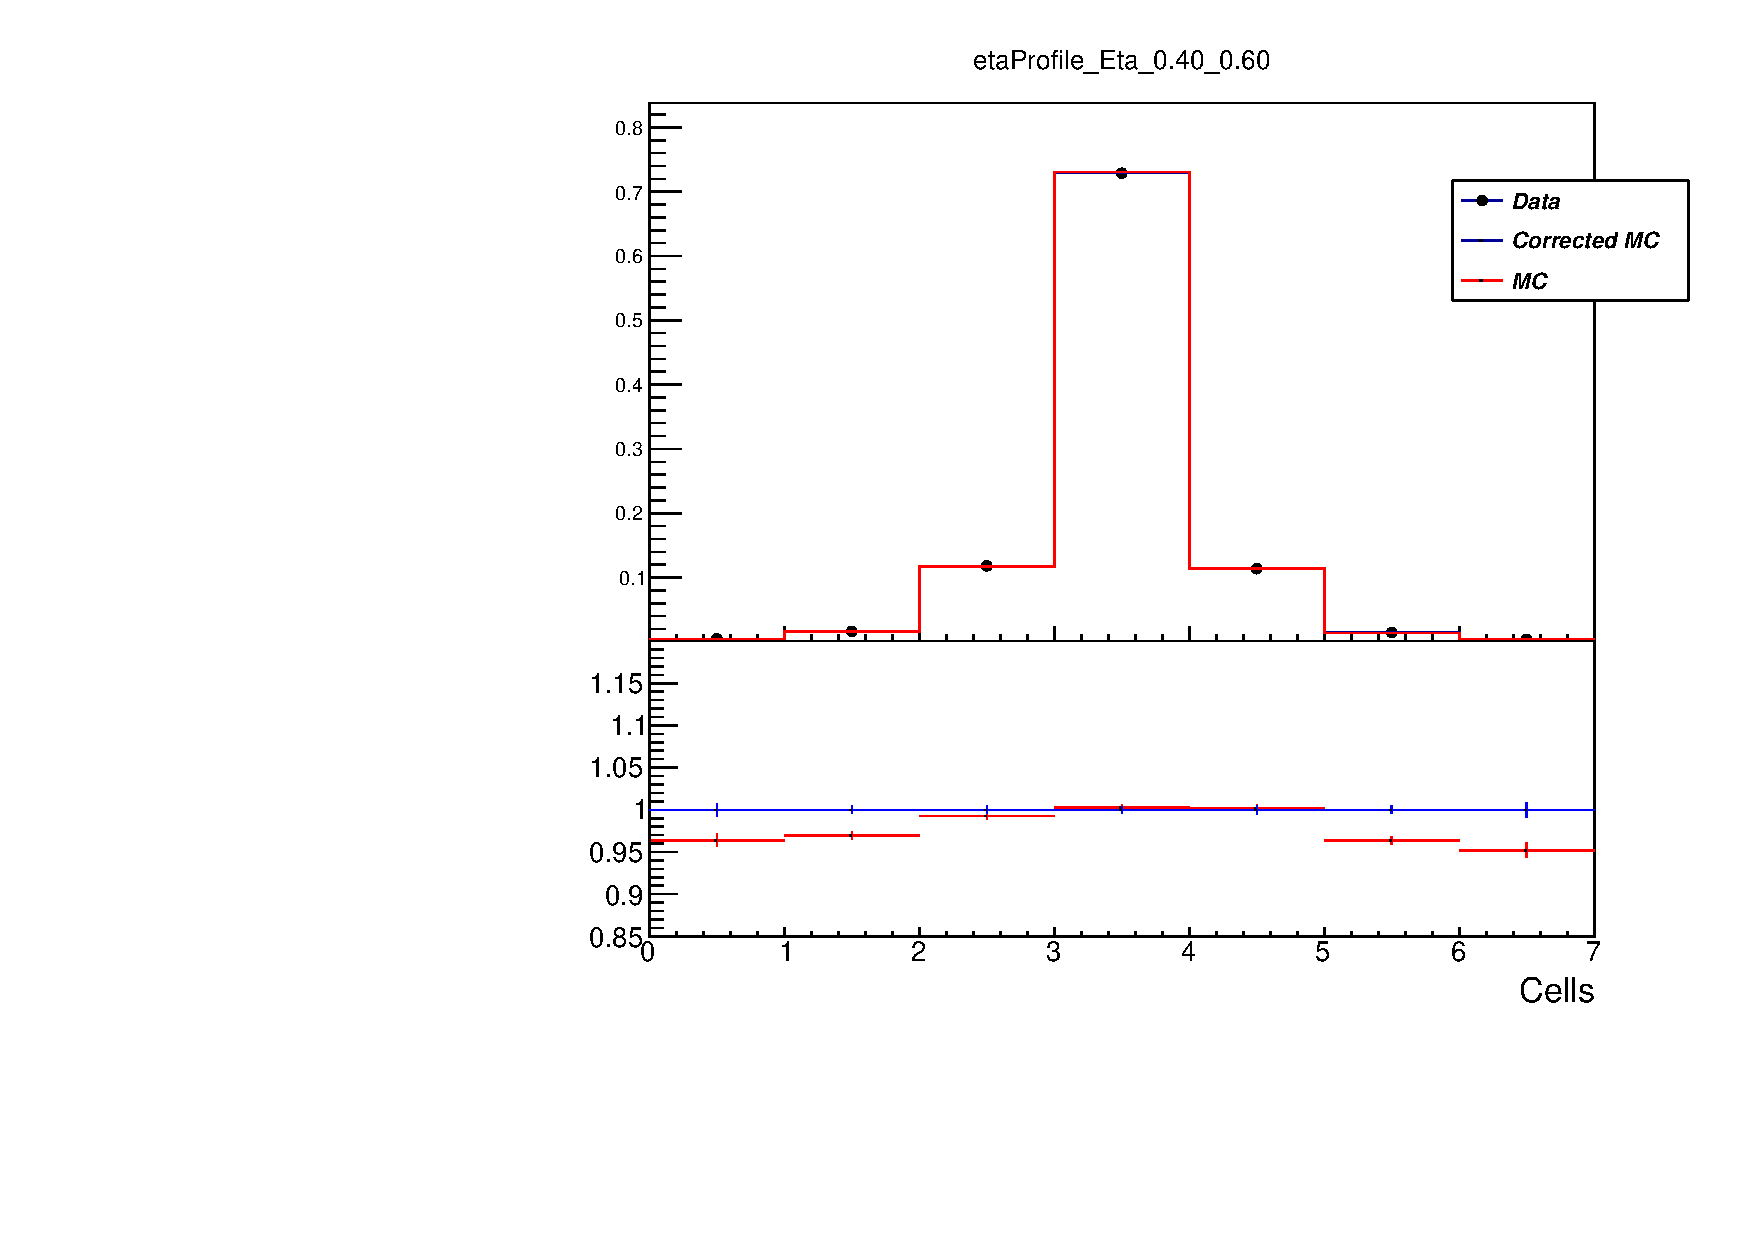
\includegraphics[width=6cm]{etaProfile_Rew_Eta_4_6_Local_Rew.pdf}\\
\column{.5\textwidth}
\centering
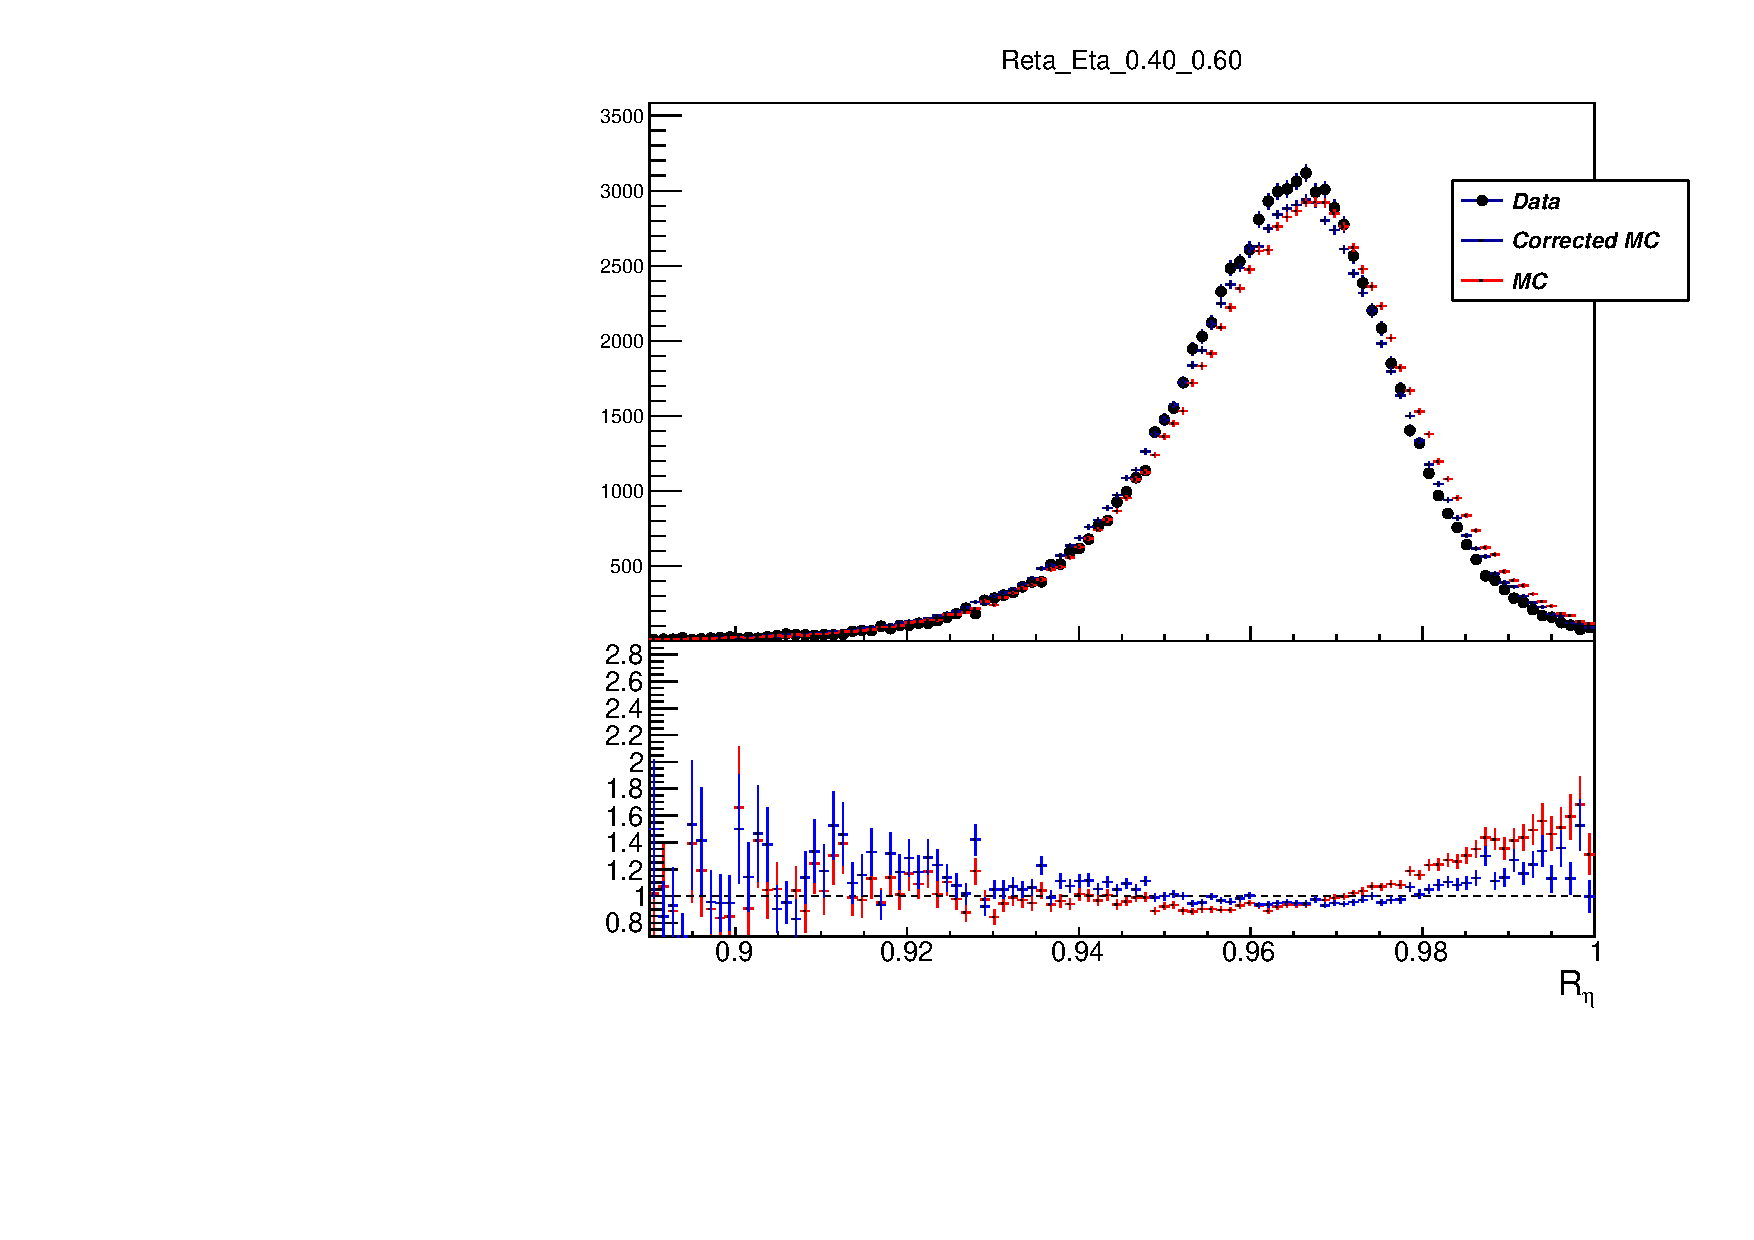
\includegraphics[width=6cm]{Reta_Rew_Eta_4_6_Local_Rew.pdf}\\

\end{columns}
\end{frame}
%------------------------------------------------
%------------------------------------------------
\begin{frame}
\frametitle{Reweighted Energy profile in $\eta$ and $R_\eta$,  $\eta \in (1.8, 2.0)$}

\begin{columns}[t]
\column{.5\textwidth}
\centering
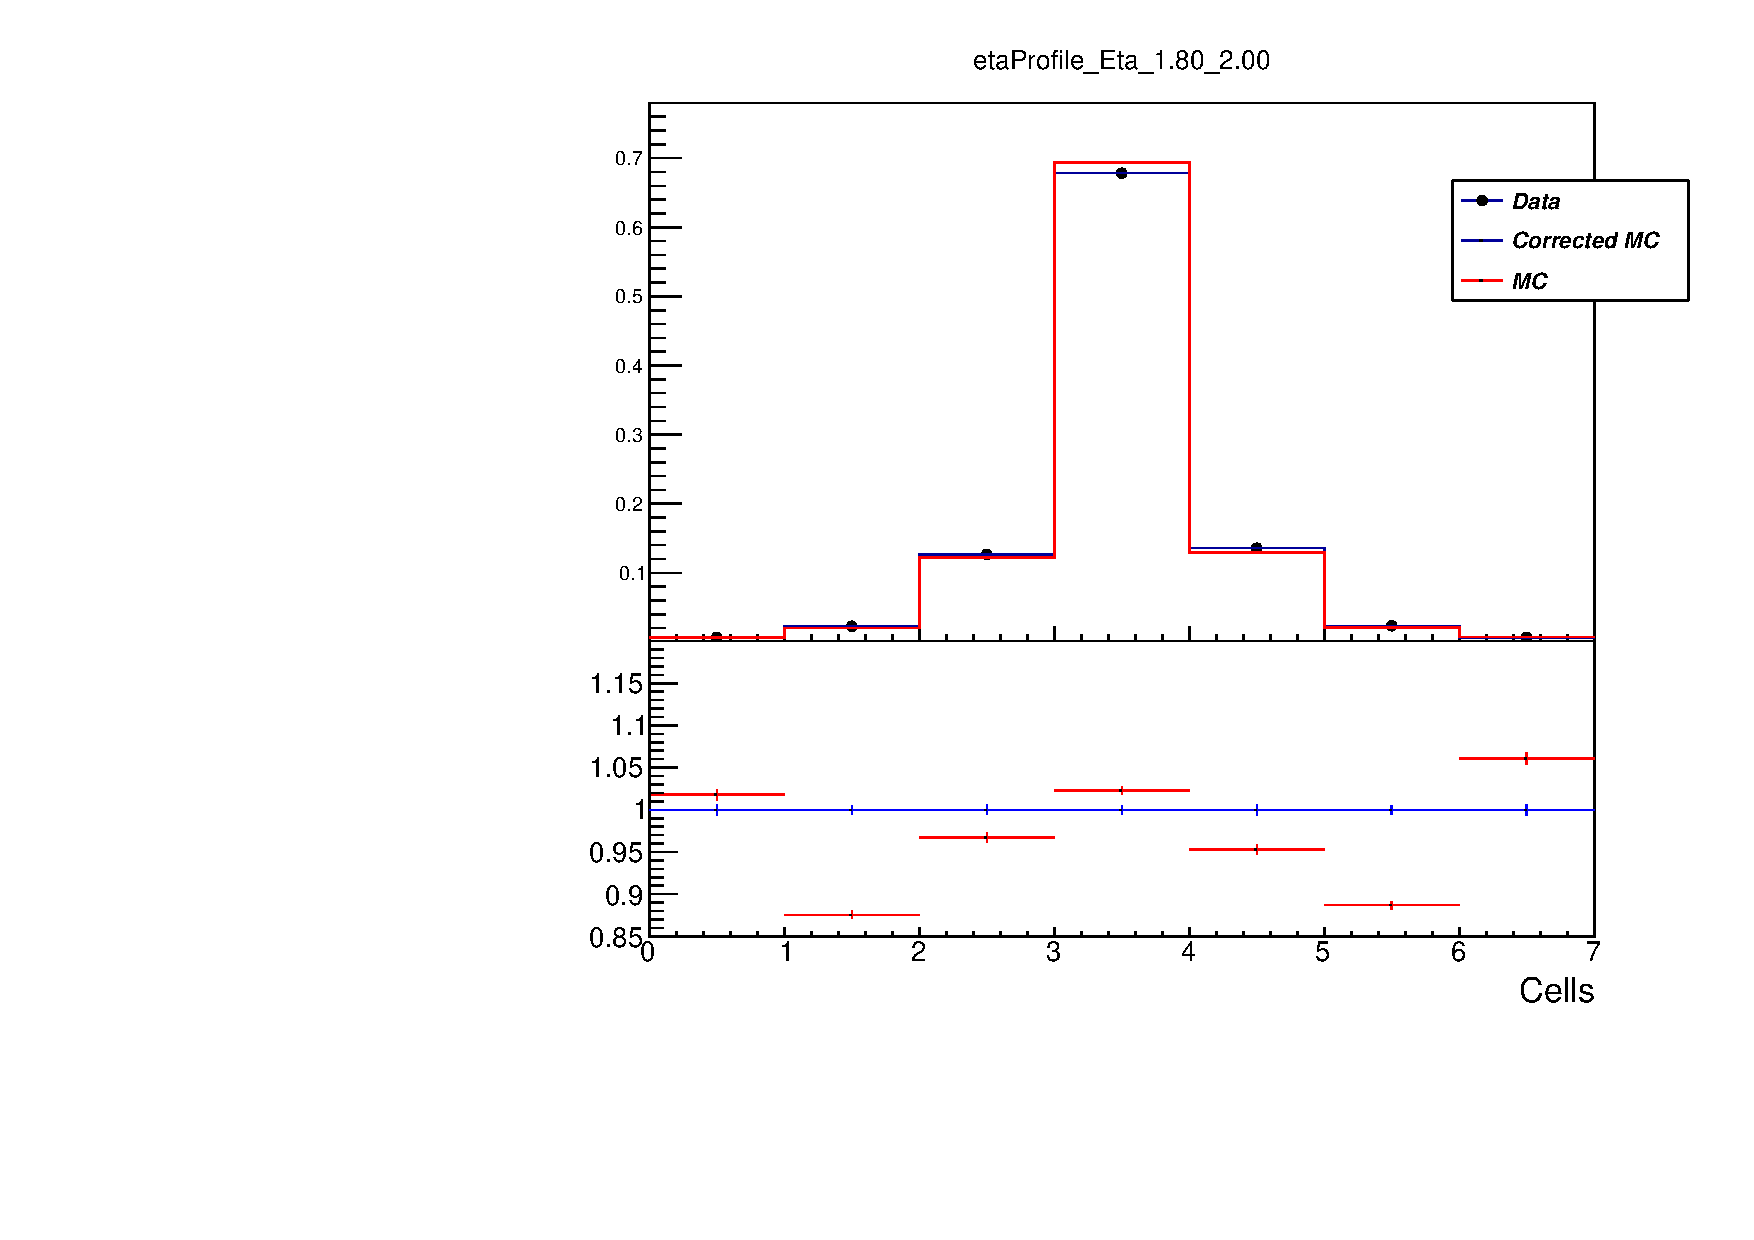
\includegraphics[width=6cm]{etaProfile_Rew_Eta_18_20_Local_Rew.pdf}

\column{.5\textwidth}
\centering
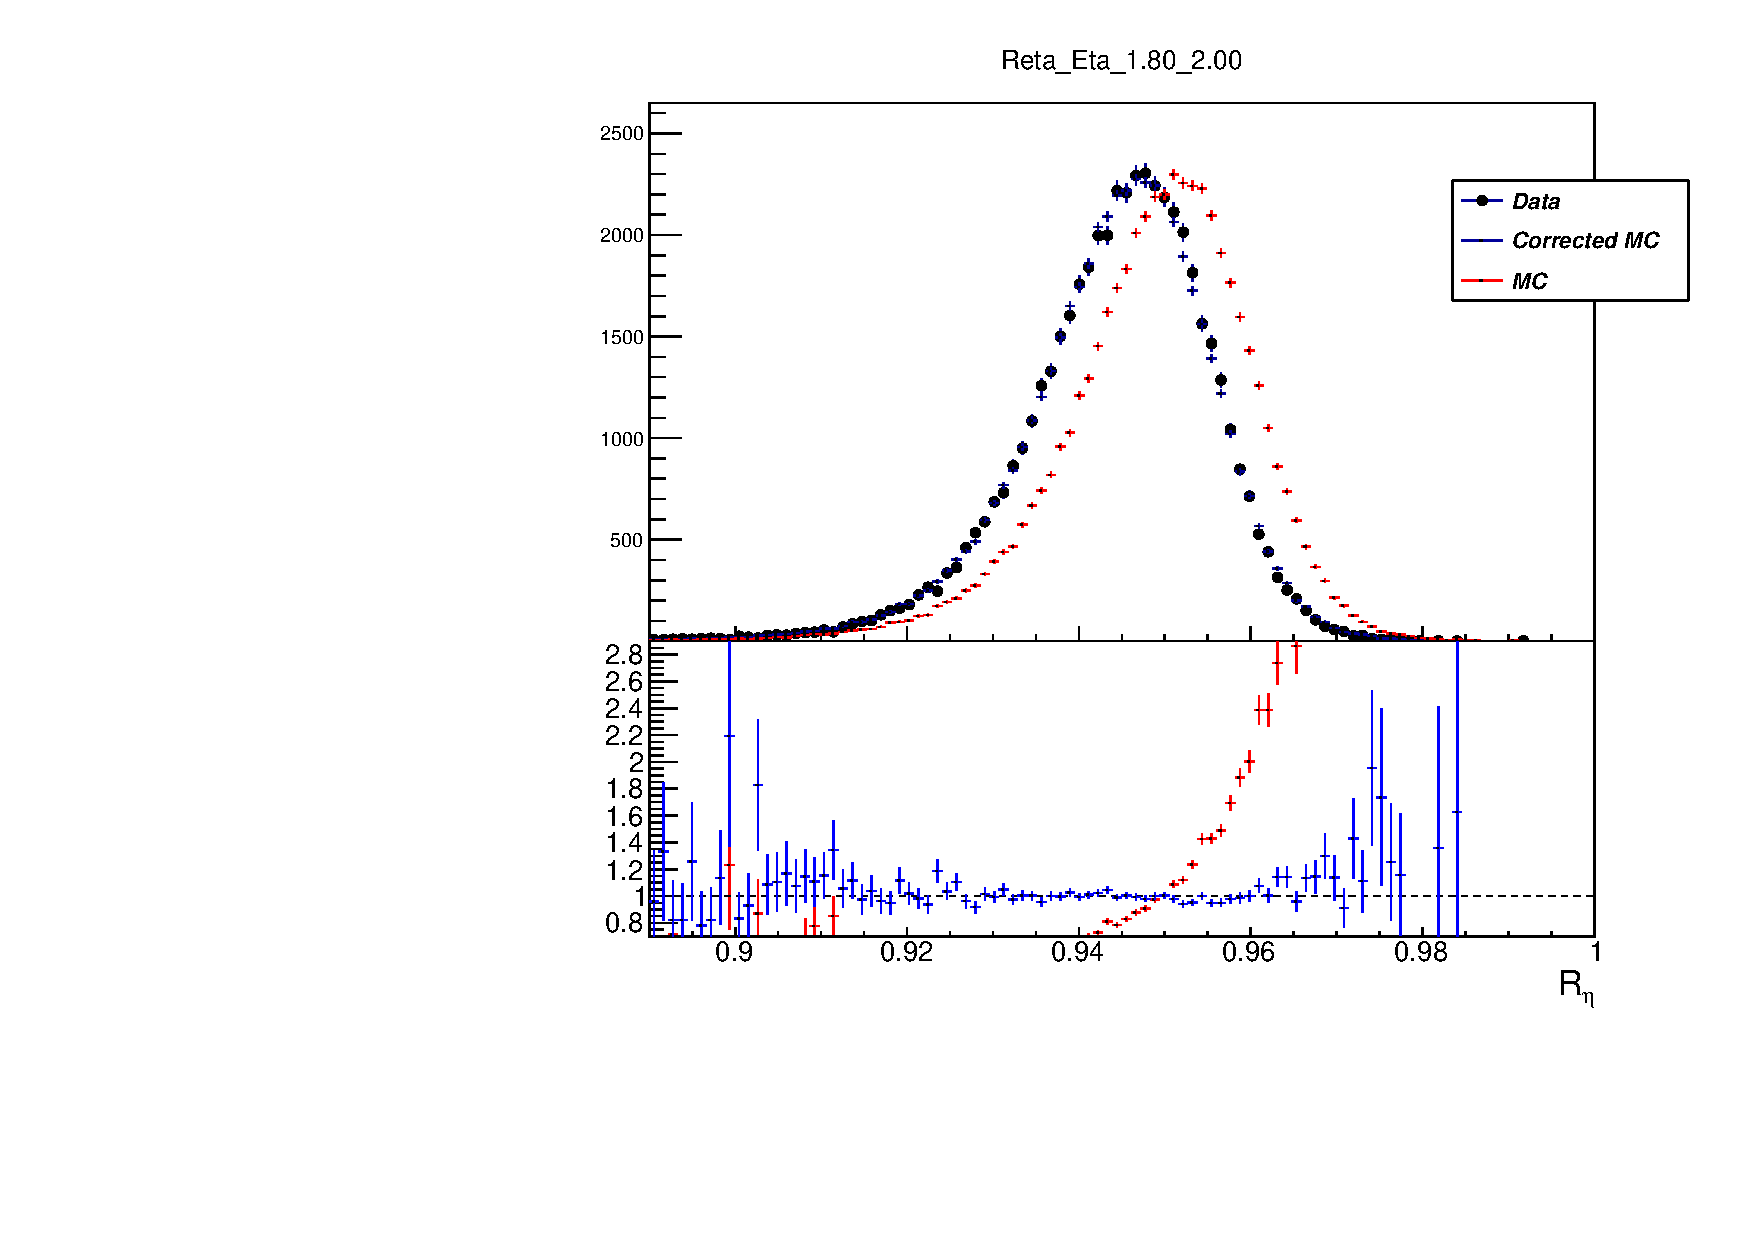
\includegraphics[width=6cm]{Reta_Rew_Eta_18_20_Local_Rew.pdf}
\end{columns}
\end{frame}
%------------------------------------------------
%------------------------------------------------
\begin{frame}
\frametitle{Reweighted energy profile in $\phi$ and $R_\phi$,  $\eta \in (0.4, 0.6)$}

\begin{columns}[t]
\column{.5\textwidth}
\centering
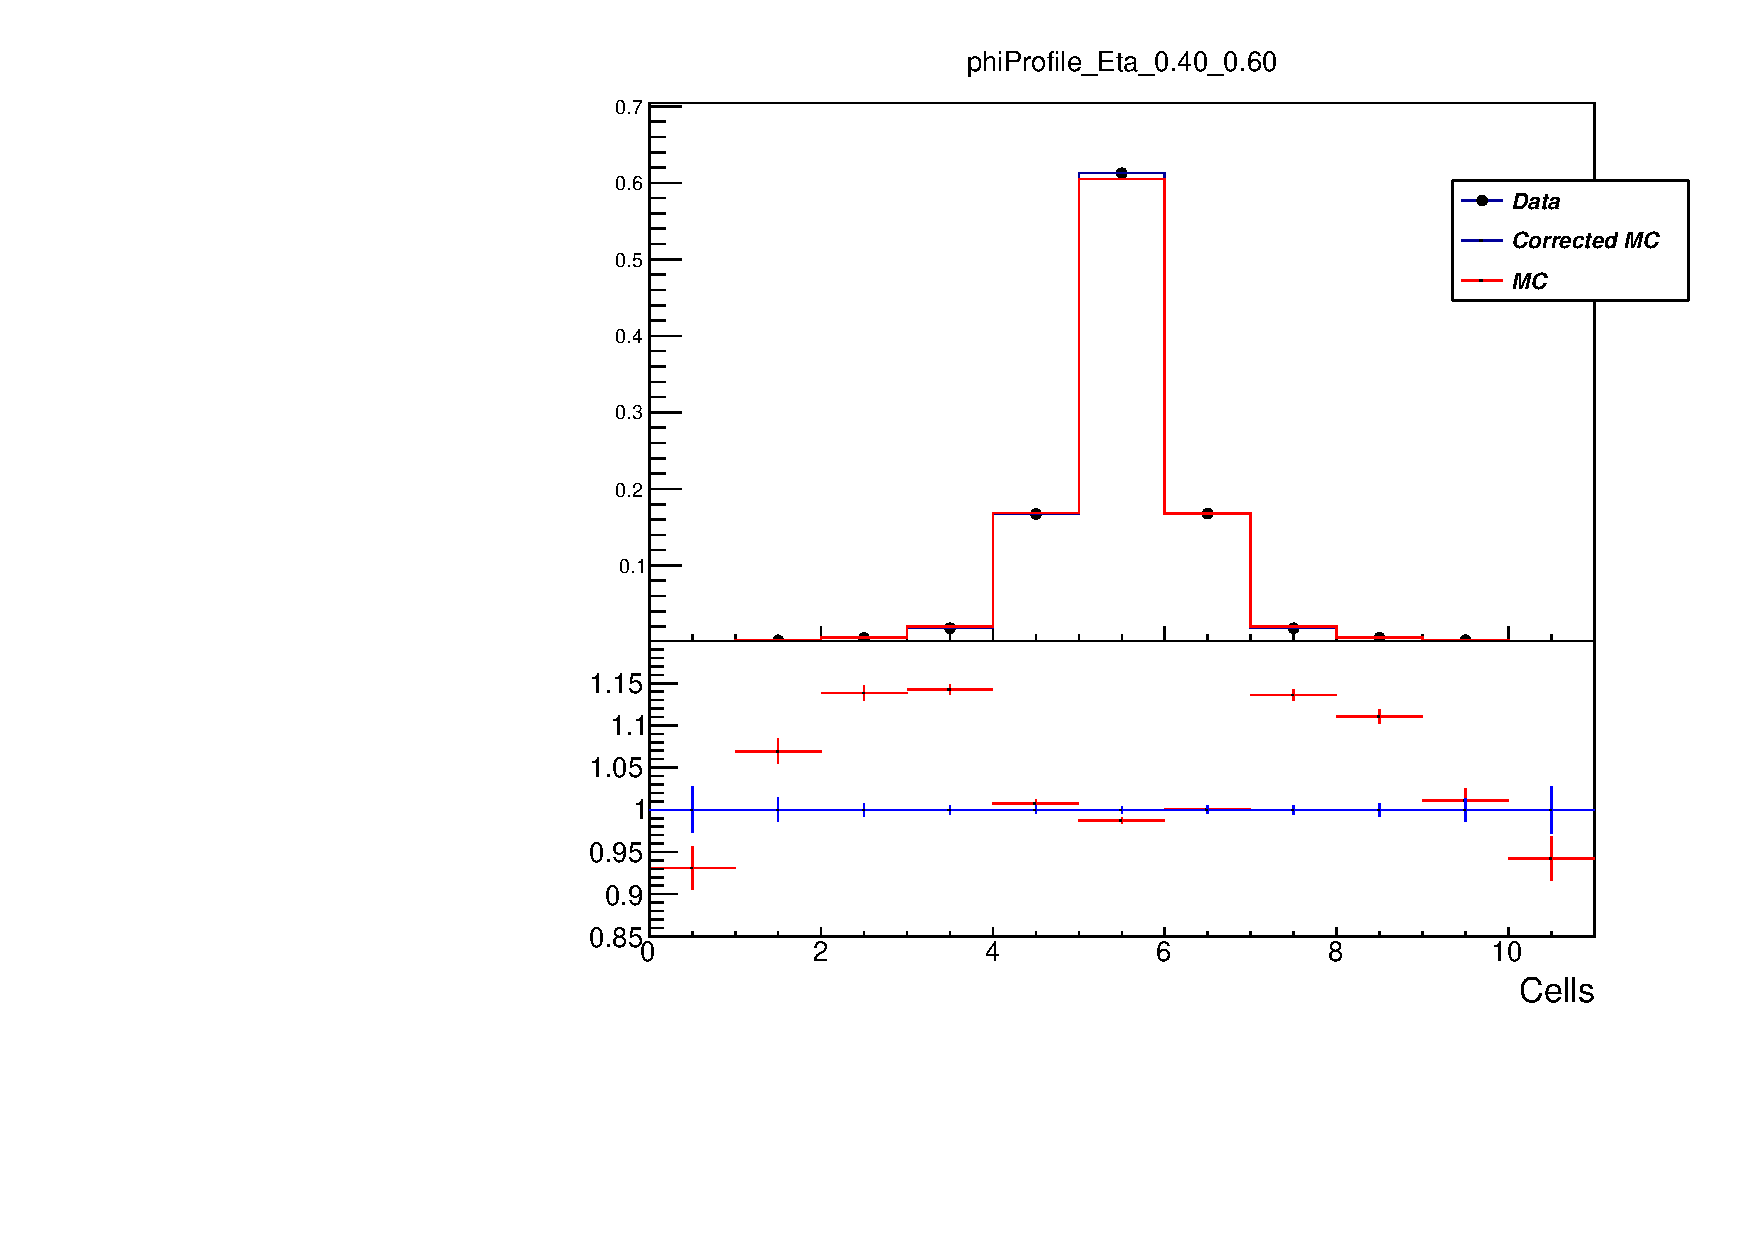
\includegraphics[width=6cm]{phiProfile_Rew_Eta_4_6_Local_Rew.pdf}\\
\column{.5\textwidth}
\centering
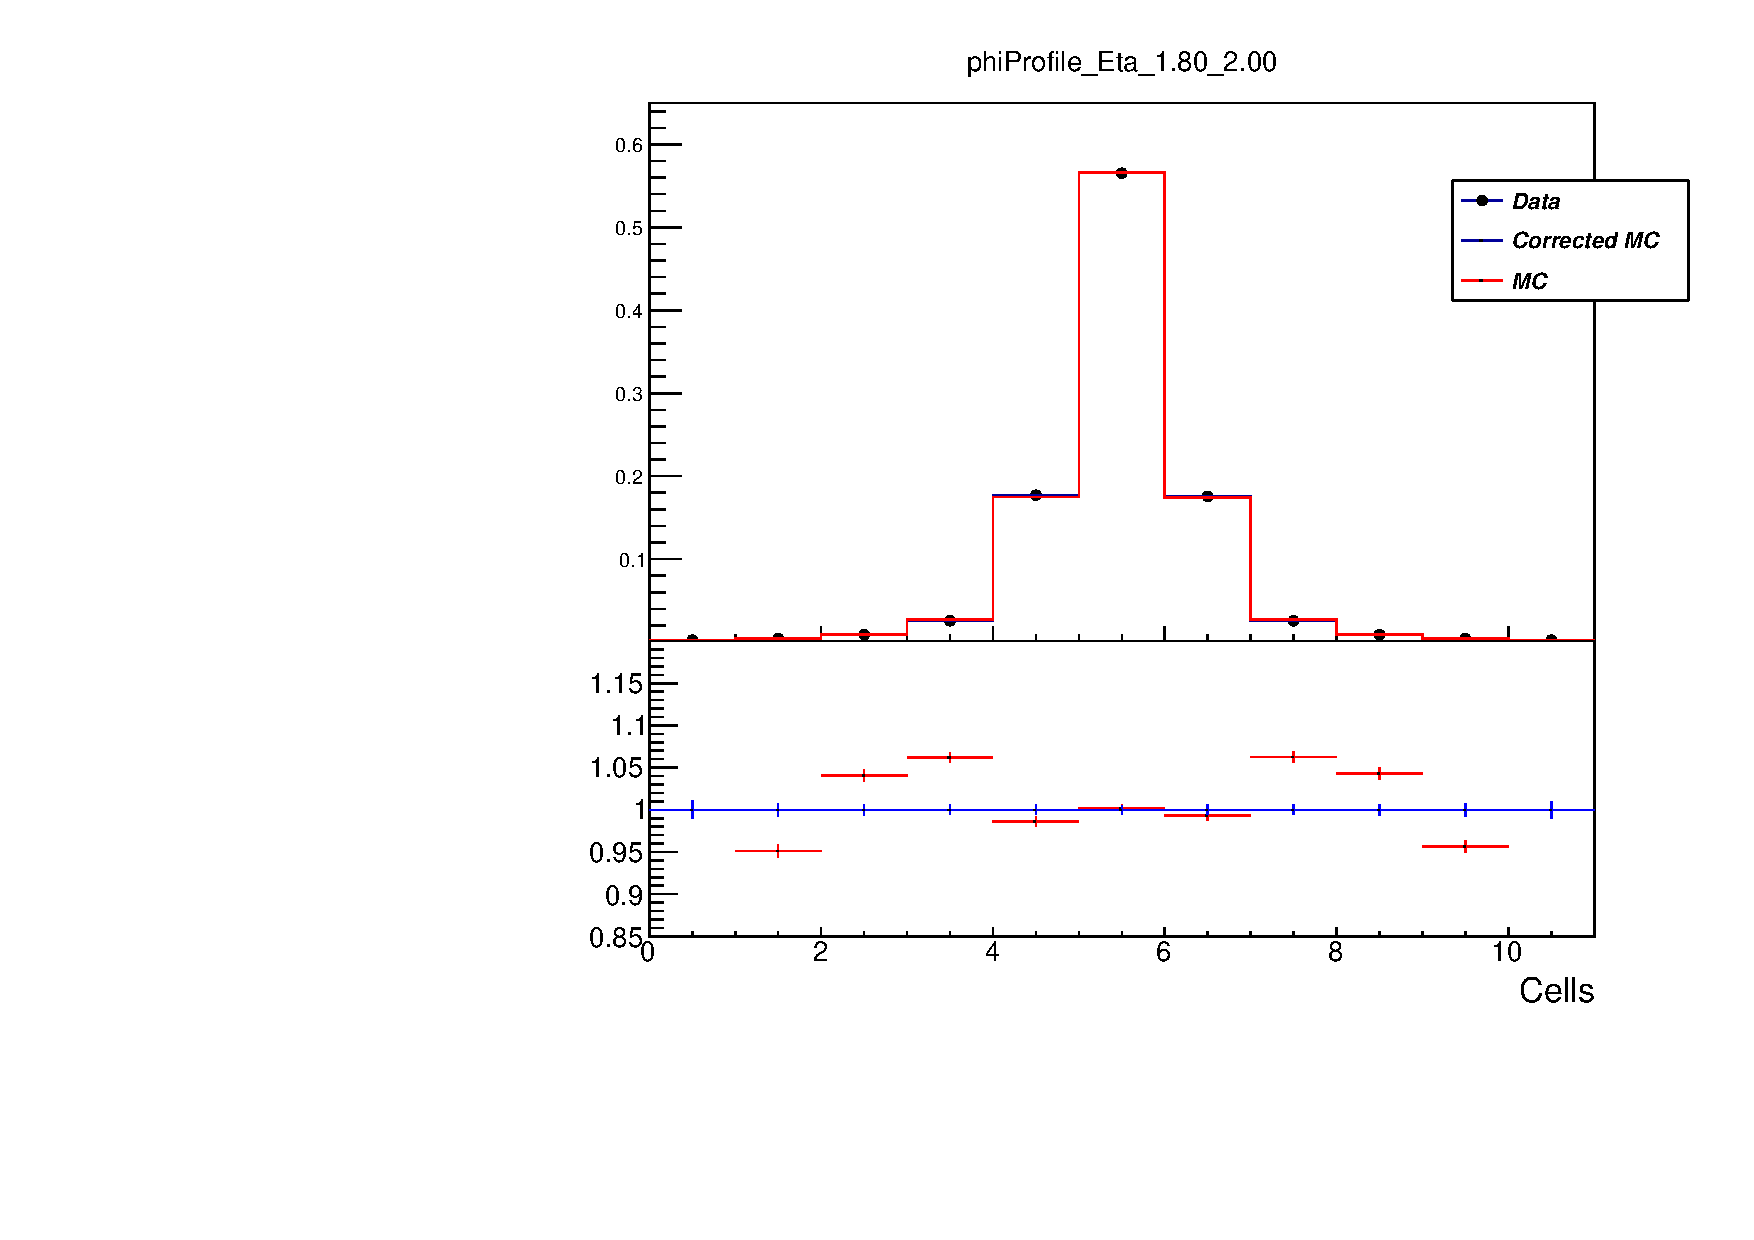
\includegraphics[width=6cm]{phiProfile_Rew_Eta_18_20_Local_Rew.pdf}
\end{columns}
\end{frame}
%------------------------------------------------

%------------------------------------------------
\begin{frame}
\frametitle{Reweighted energy profile in $\phi$ and $R_\phi$,  $\eta \in (1.8, 2.0)$}

\begin{columns}[t]
\column{.5\textwidth}
\centering
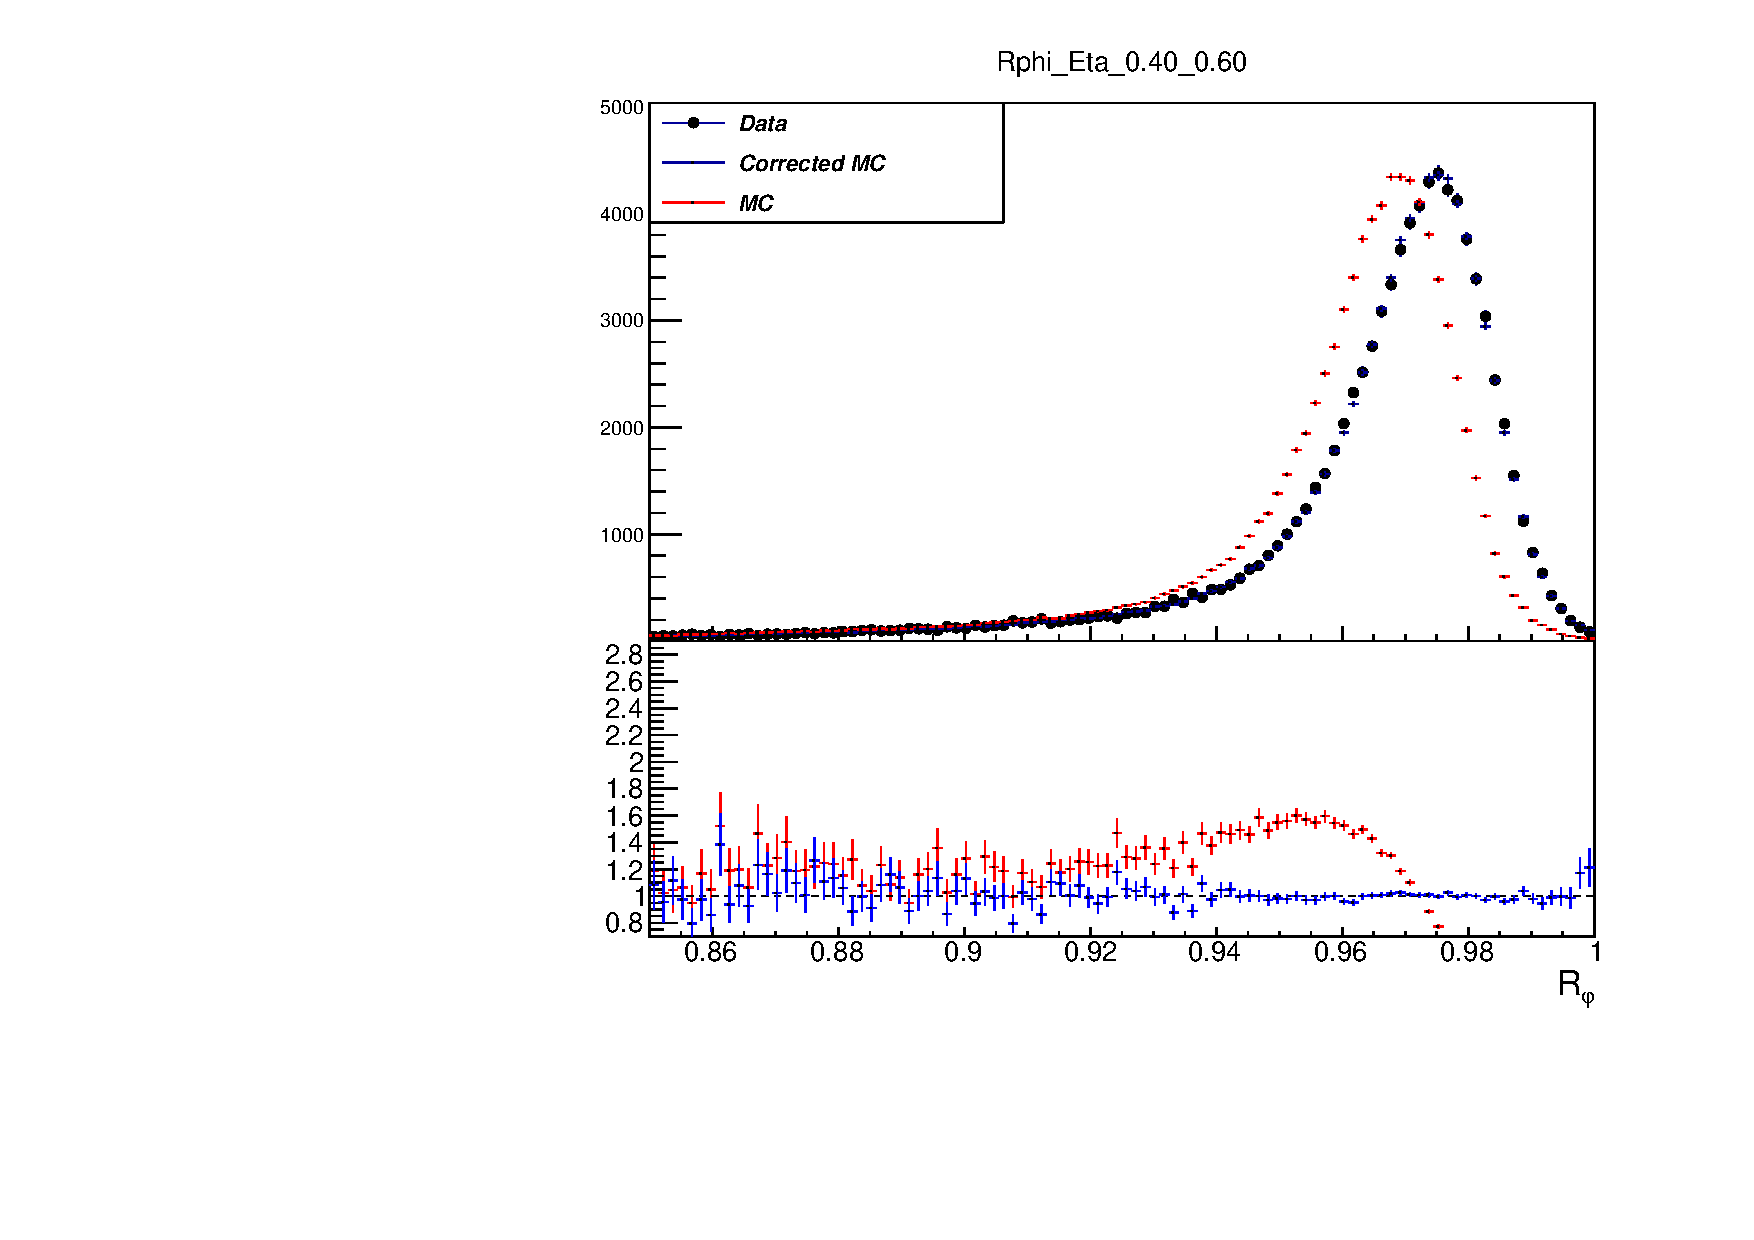
\includegraphics[width=6cm]{Rphi_Rew_Eta_4_6_Local_Rew.pdf}\\
\column{.5\textwidth}
\centering
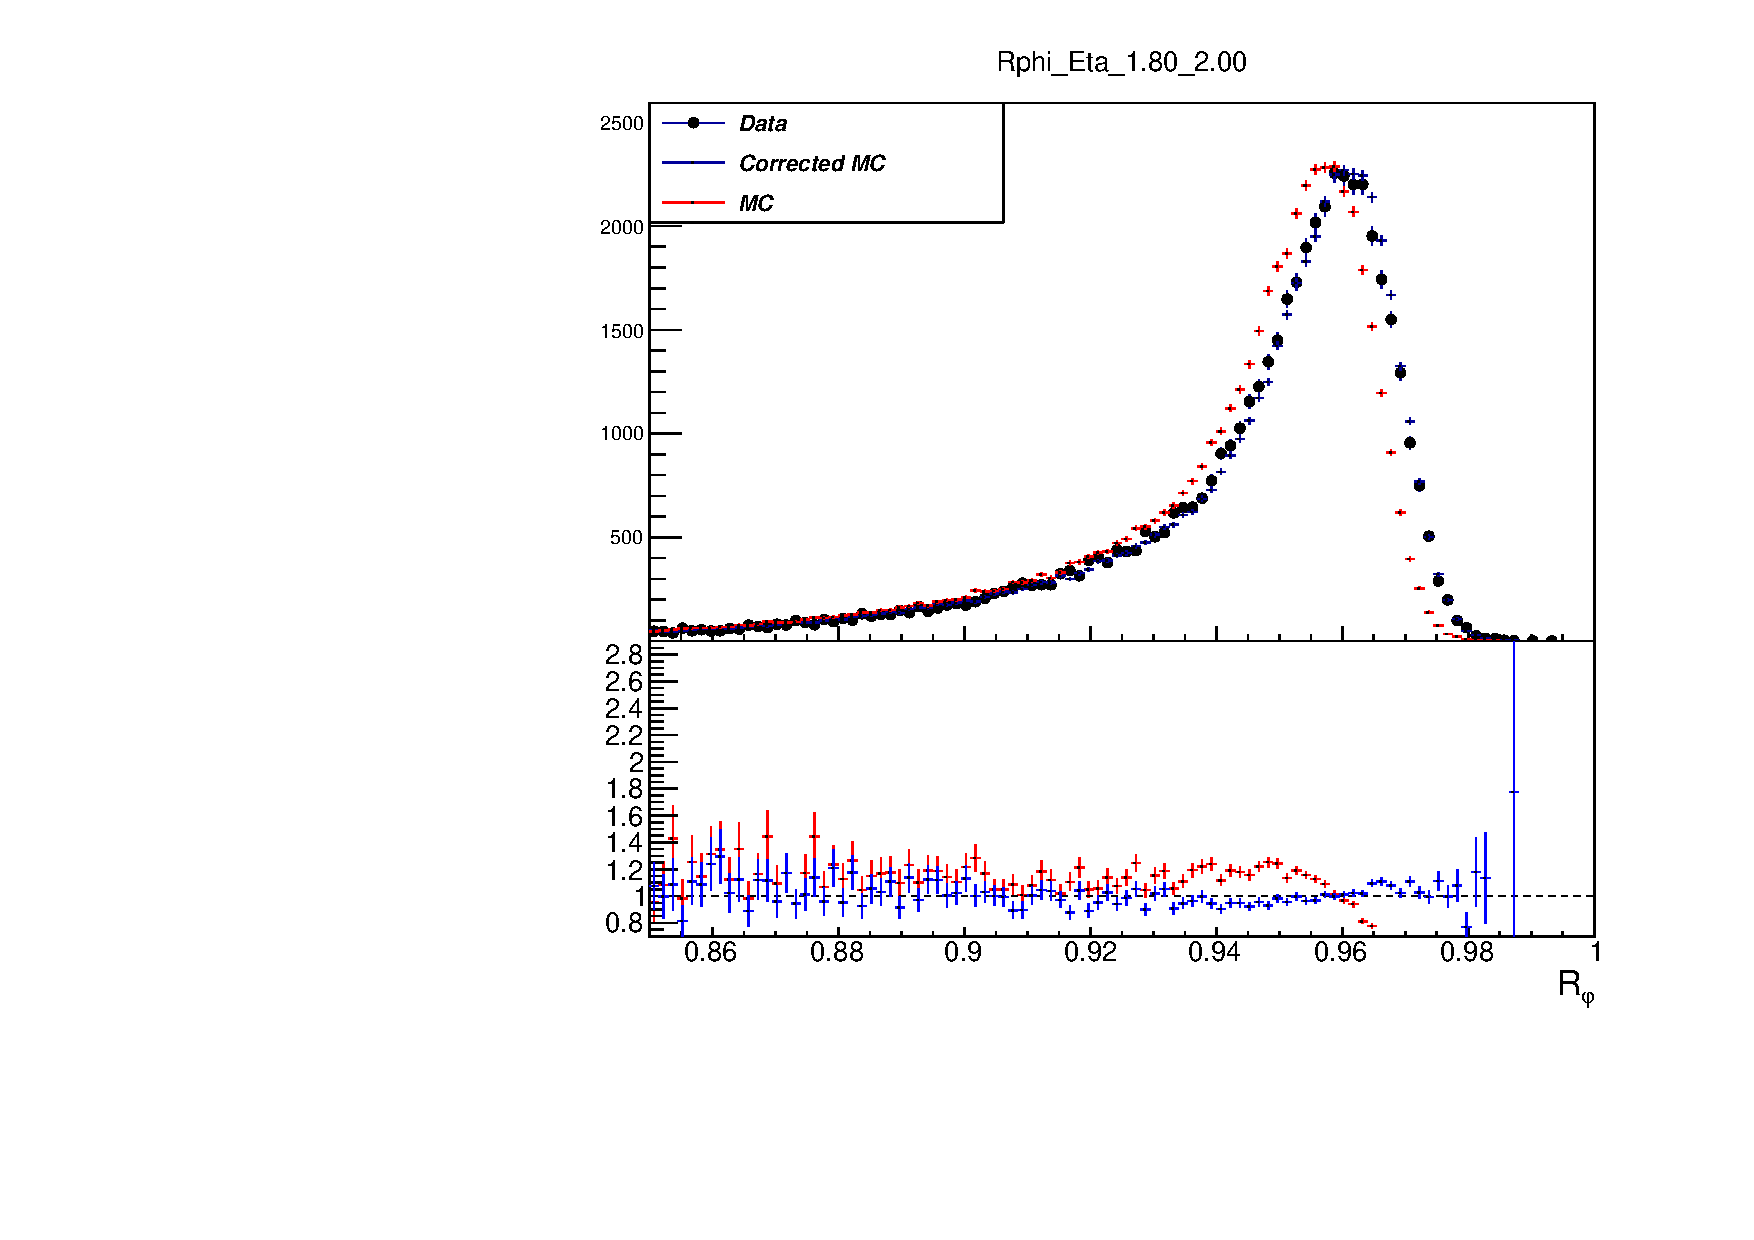
\includegraphics[width=6cm]{Rphi_Rew_Eta_18_20_Local_Rew.pdf}
\end{columns}
\end{frame}
%------------------------------------------------
%------------------------------------------------
\begin{frame}
\frametitle{Reweighting steps}
\begin{itemize}
\item Local closure test \textcolor{red}{ $\checkmark$}\\

\end{itemize}
\end{frame}
%------------------------------------------------
%------------------------------------------------
\begin{frame}
\frametitle{Phi profile - $e^-$/$e^+$ ratio, Data and MC are in agreement}

\begin{columns}[t]
\column{.5\textwidth}
\centering
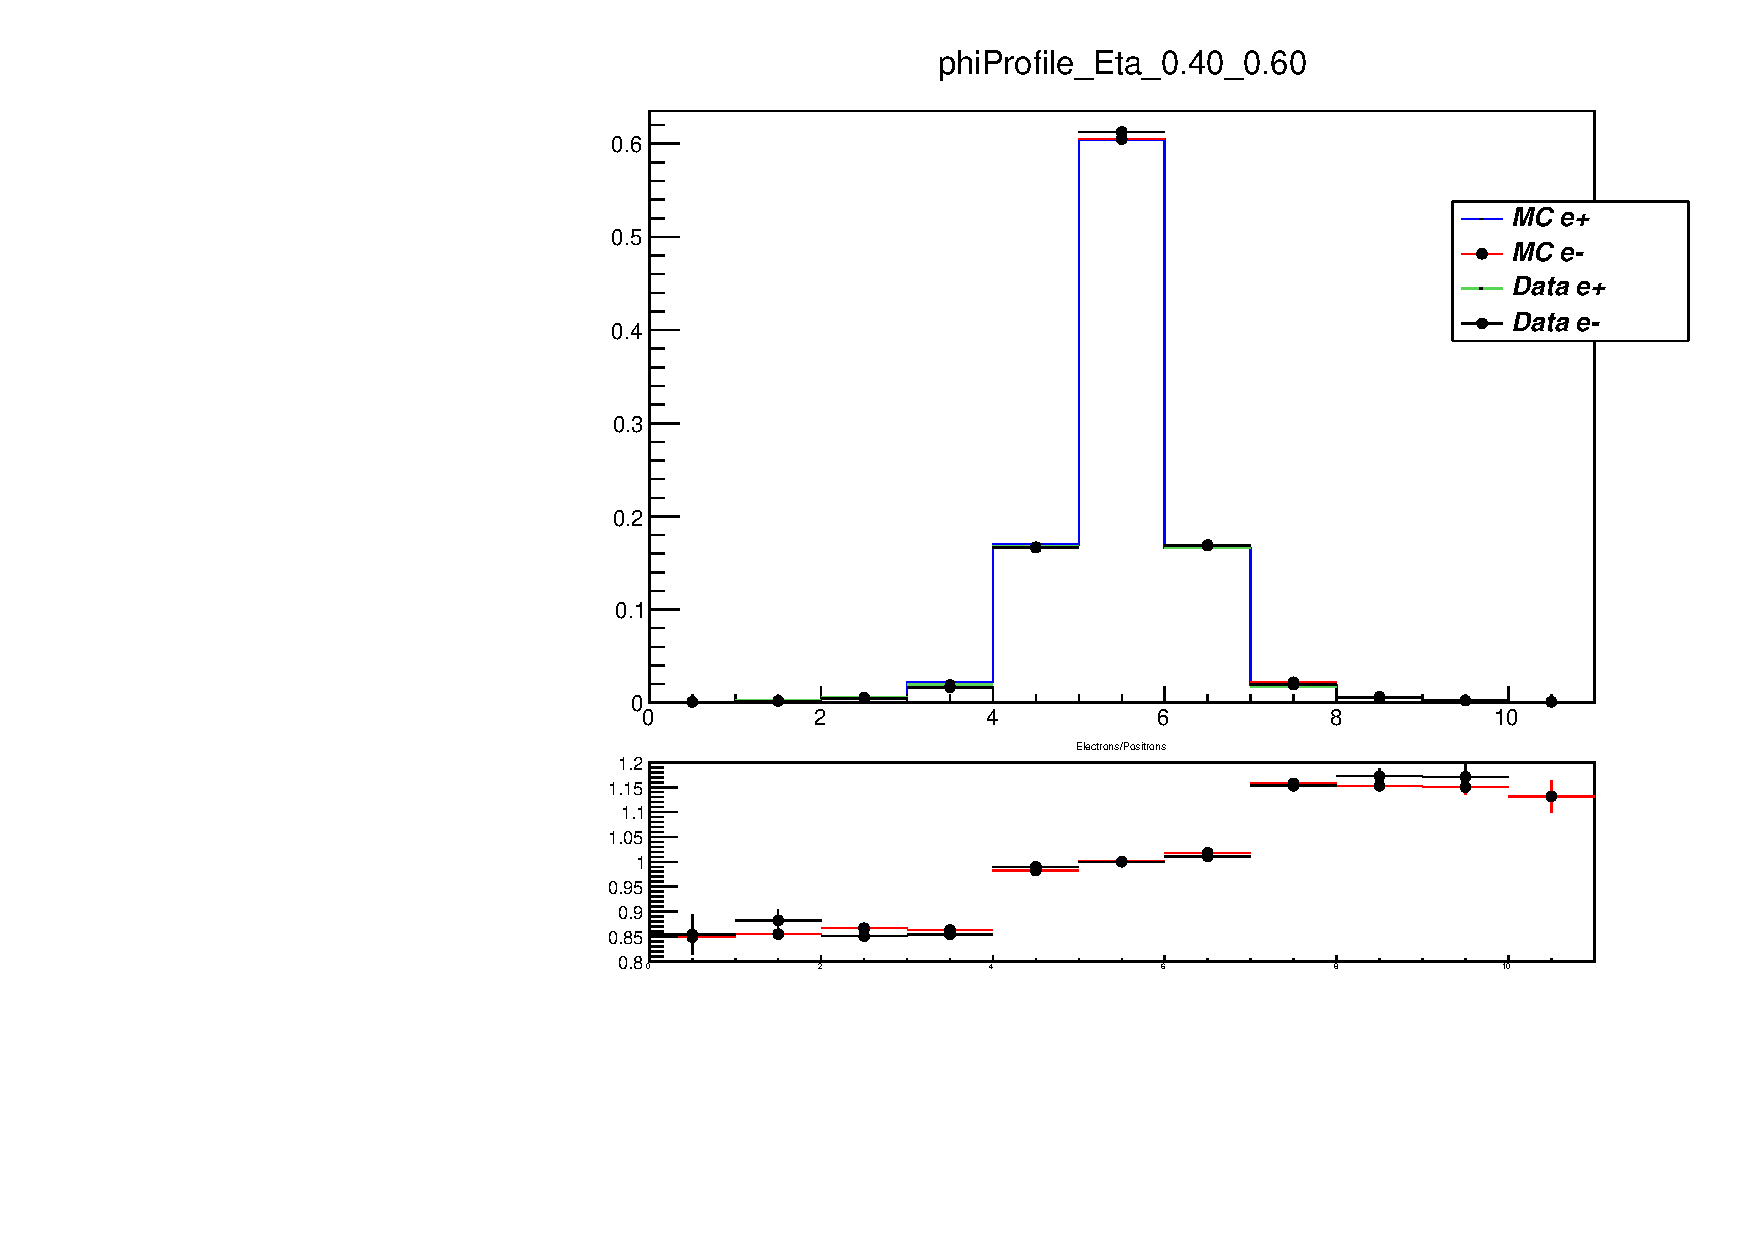
\includegraphics[width=6cm,height=4cm]{phiProfileDataMC_Eta_4_6.pdf}\\
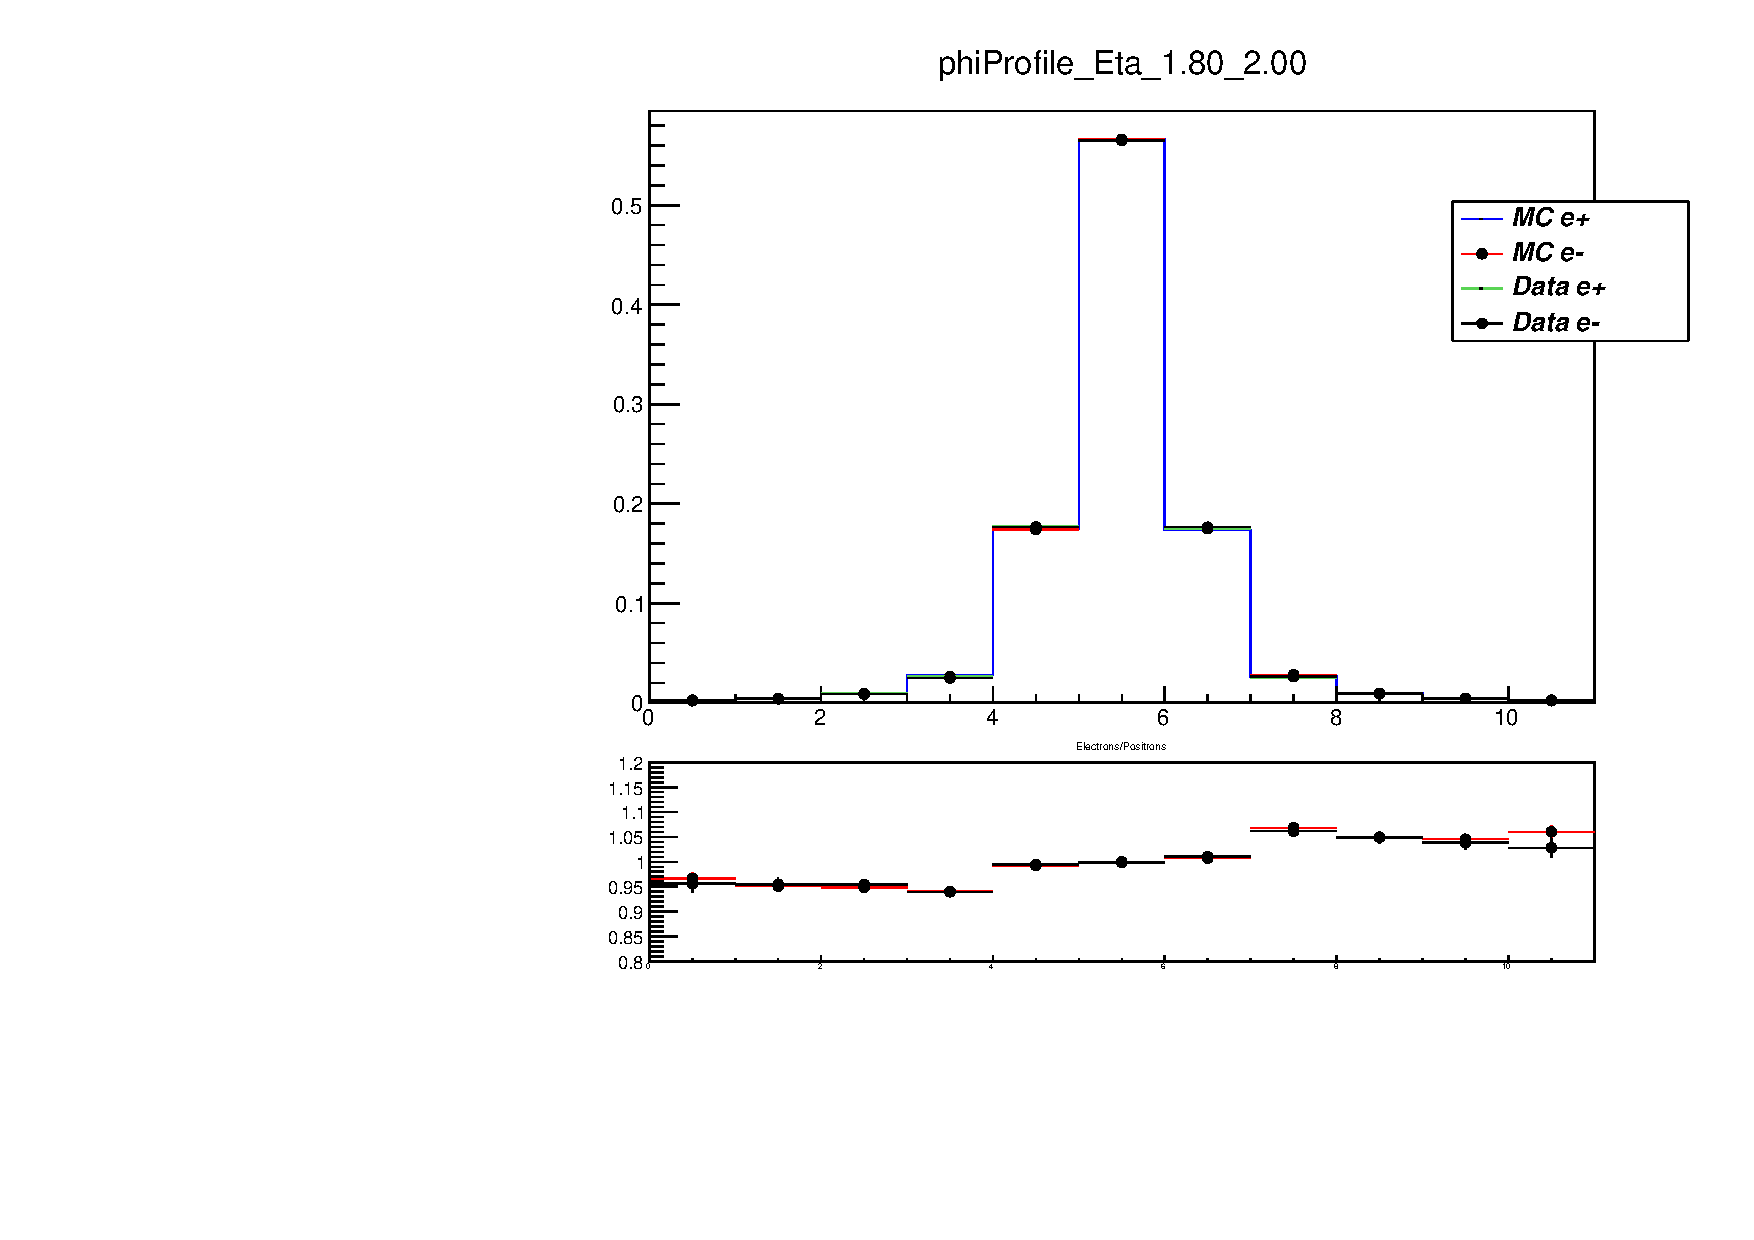
\includegraphics[width=6cm,height=4cm]{phiProfileDataMC_Eta_18_20.pdf}
\column{.5\textwidth}
\centering
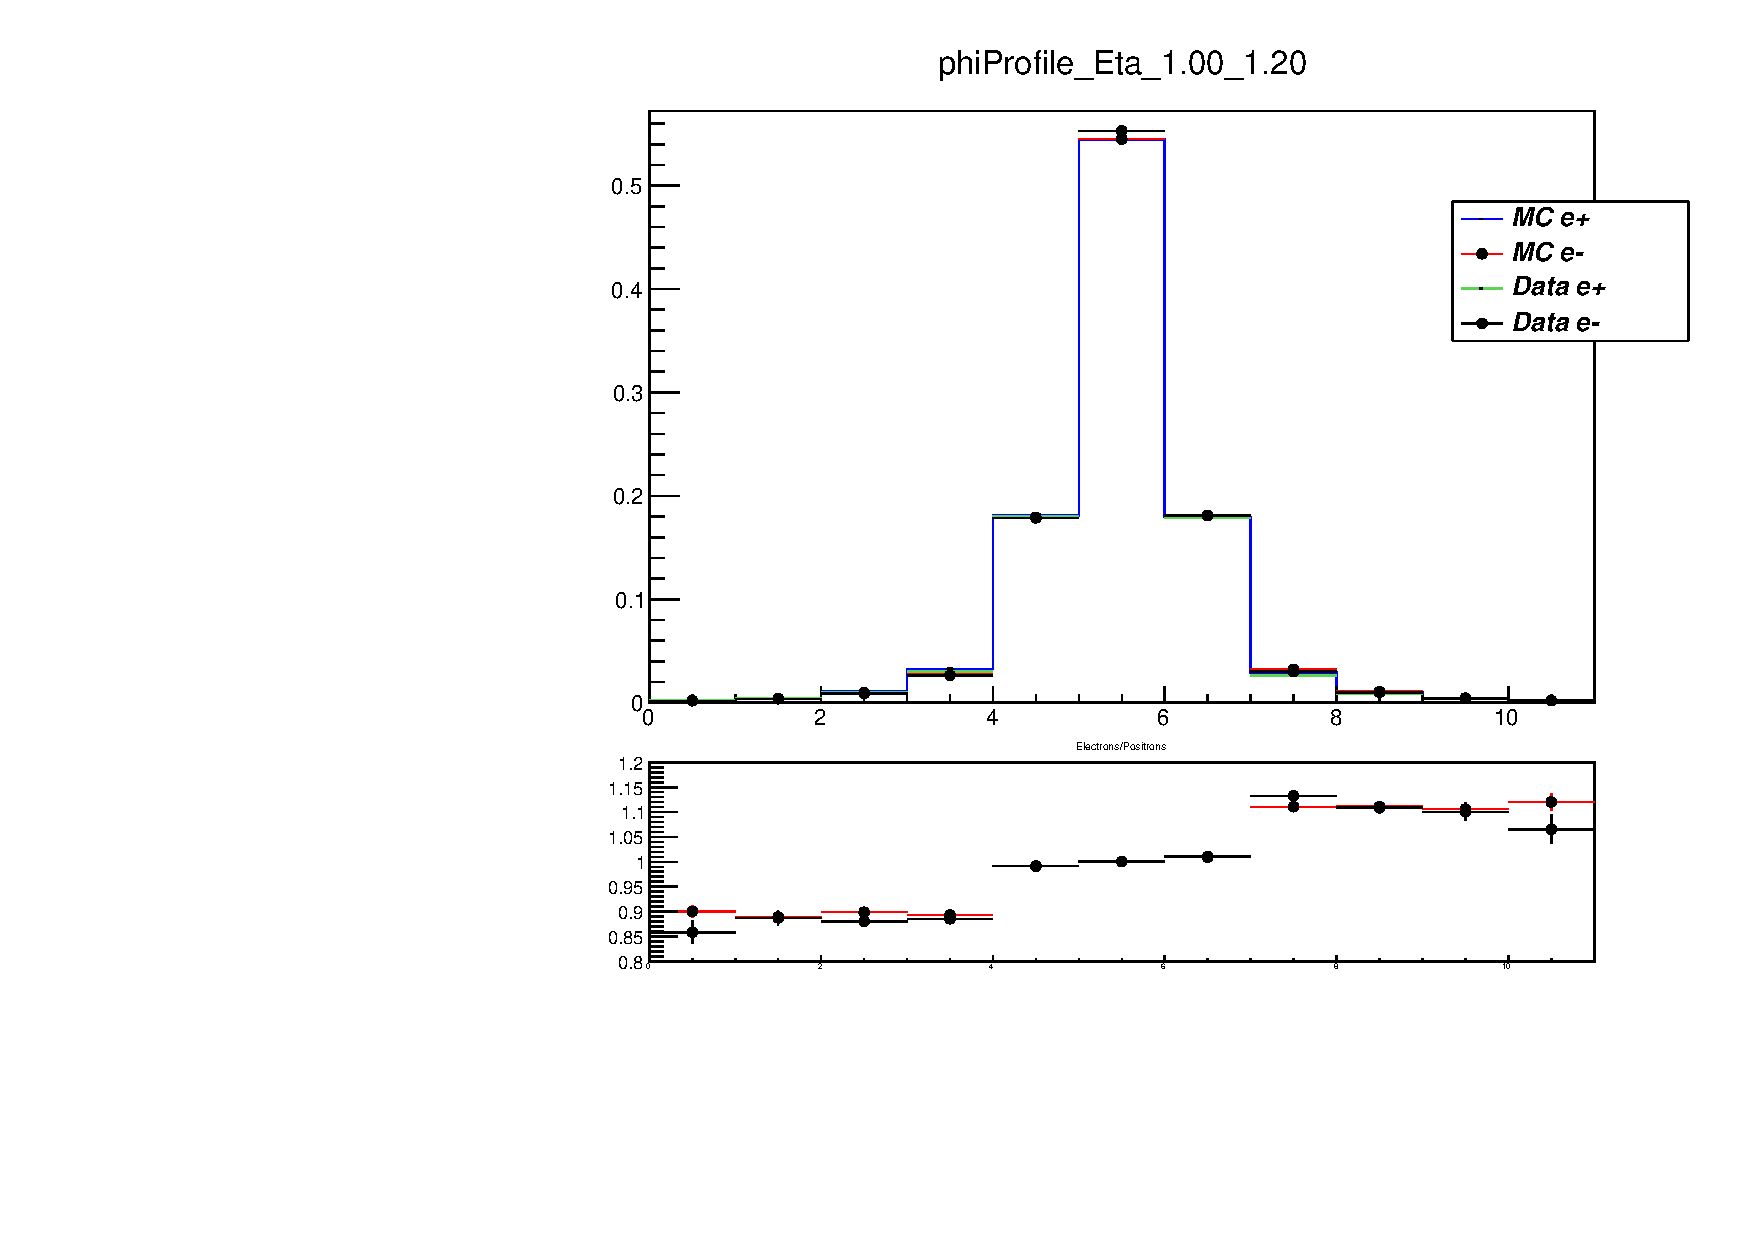
\includegraphics[width=6cm,height=4cm]{phiProfileDataMC_Eta_10_12.pdf}\\
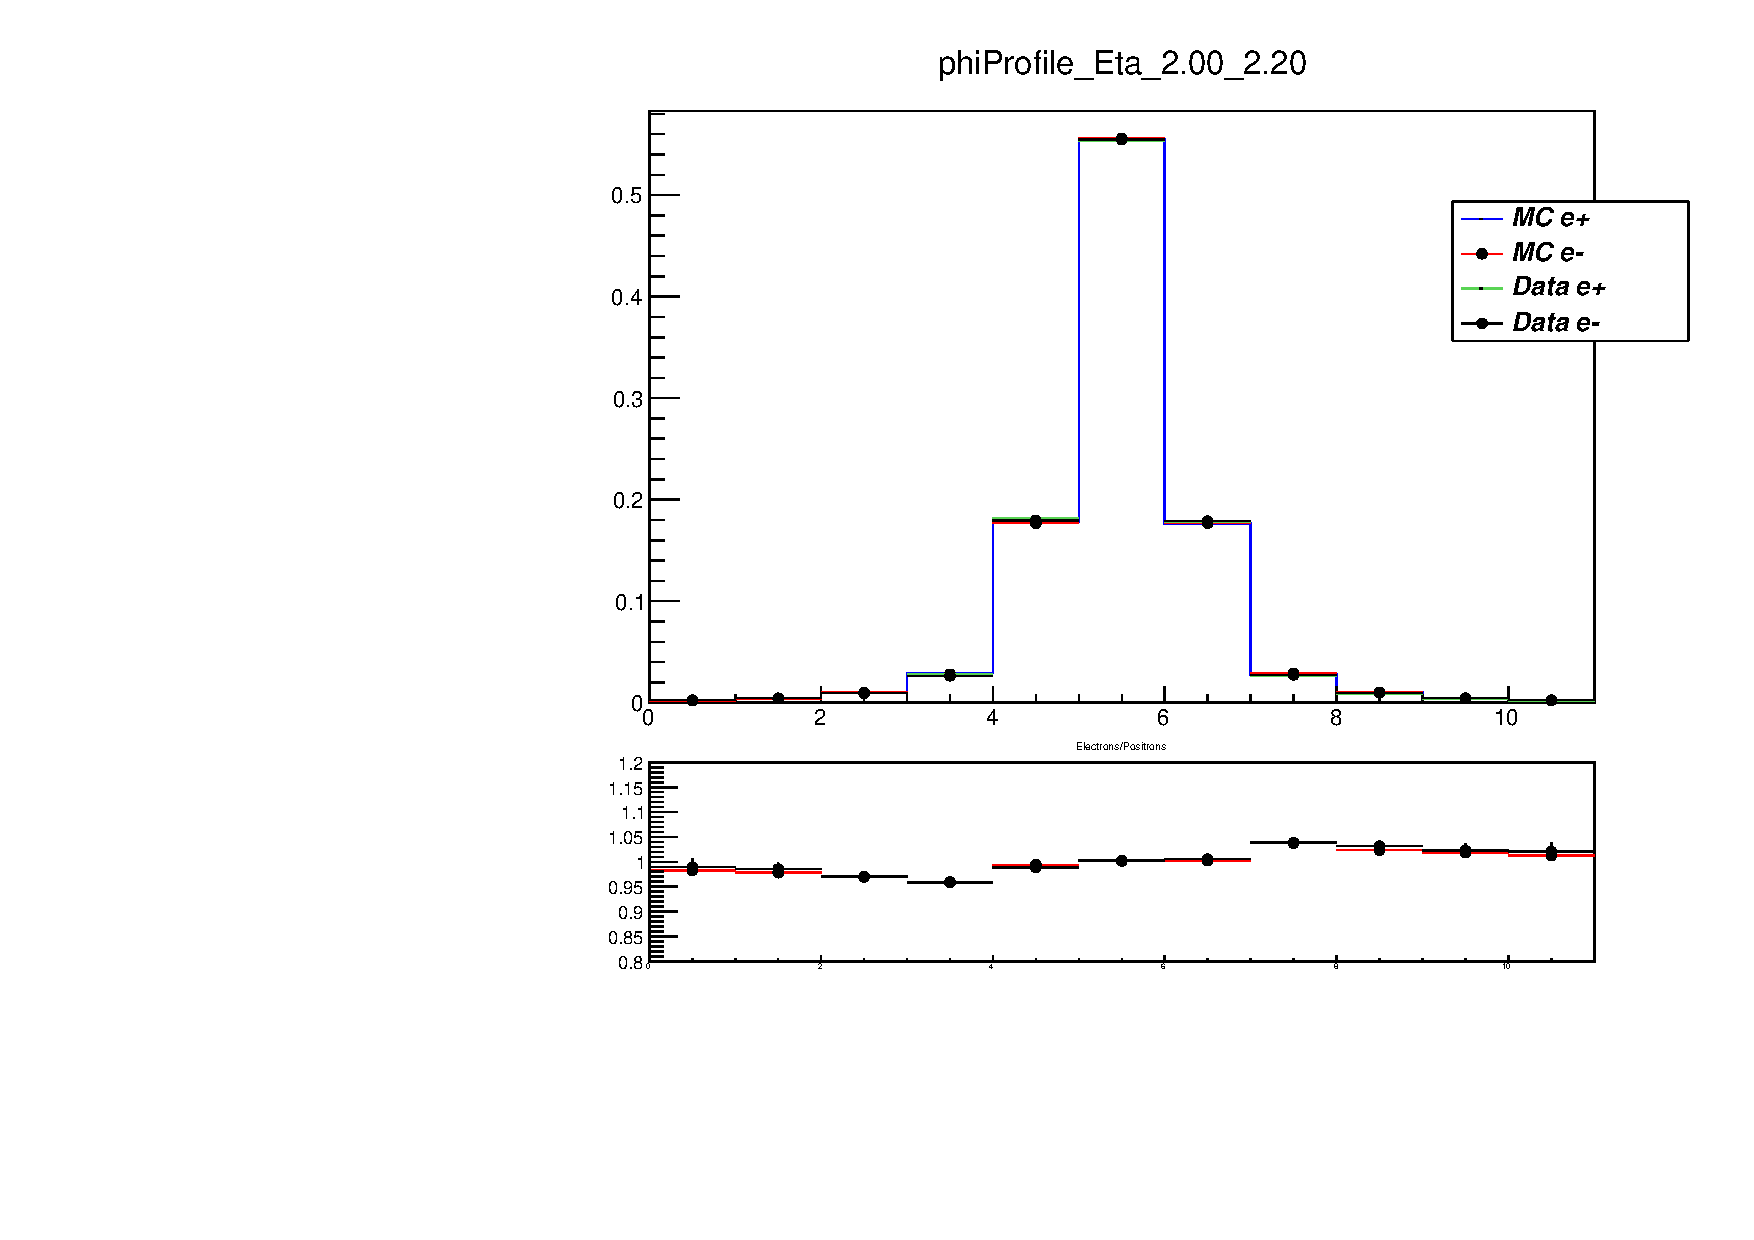
\includegraphics[width=6cm,height=4cm]{phiProfileDataMC_Eta_20_22.pdf}
\end{columns}
\end{frame}
%------------------------------------------------


%------------------------------------------------
\begin{frame}
\frametitle{Schematic Bremsstrahlung profile}
\centering
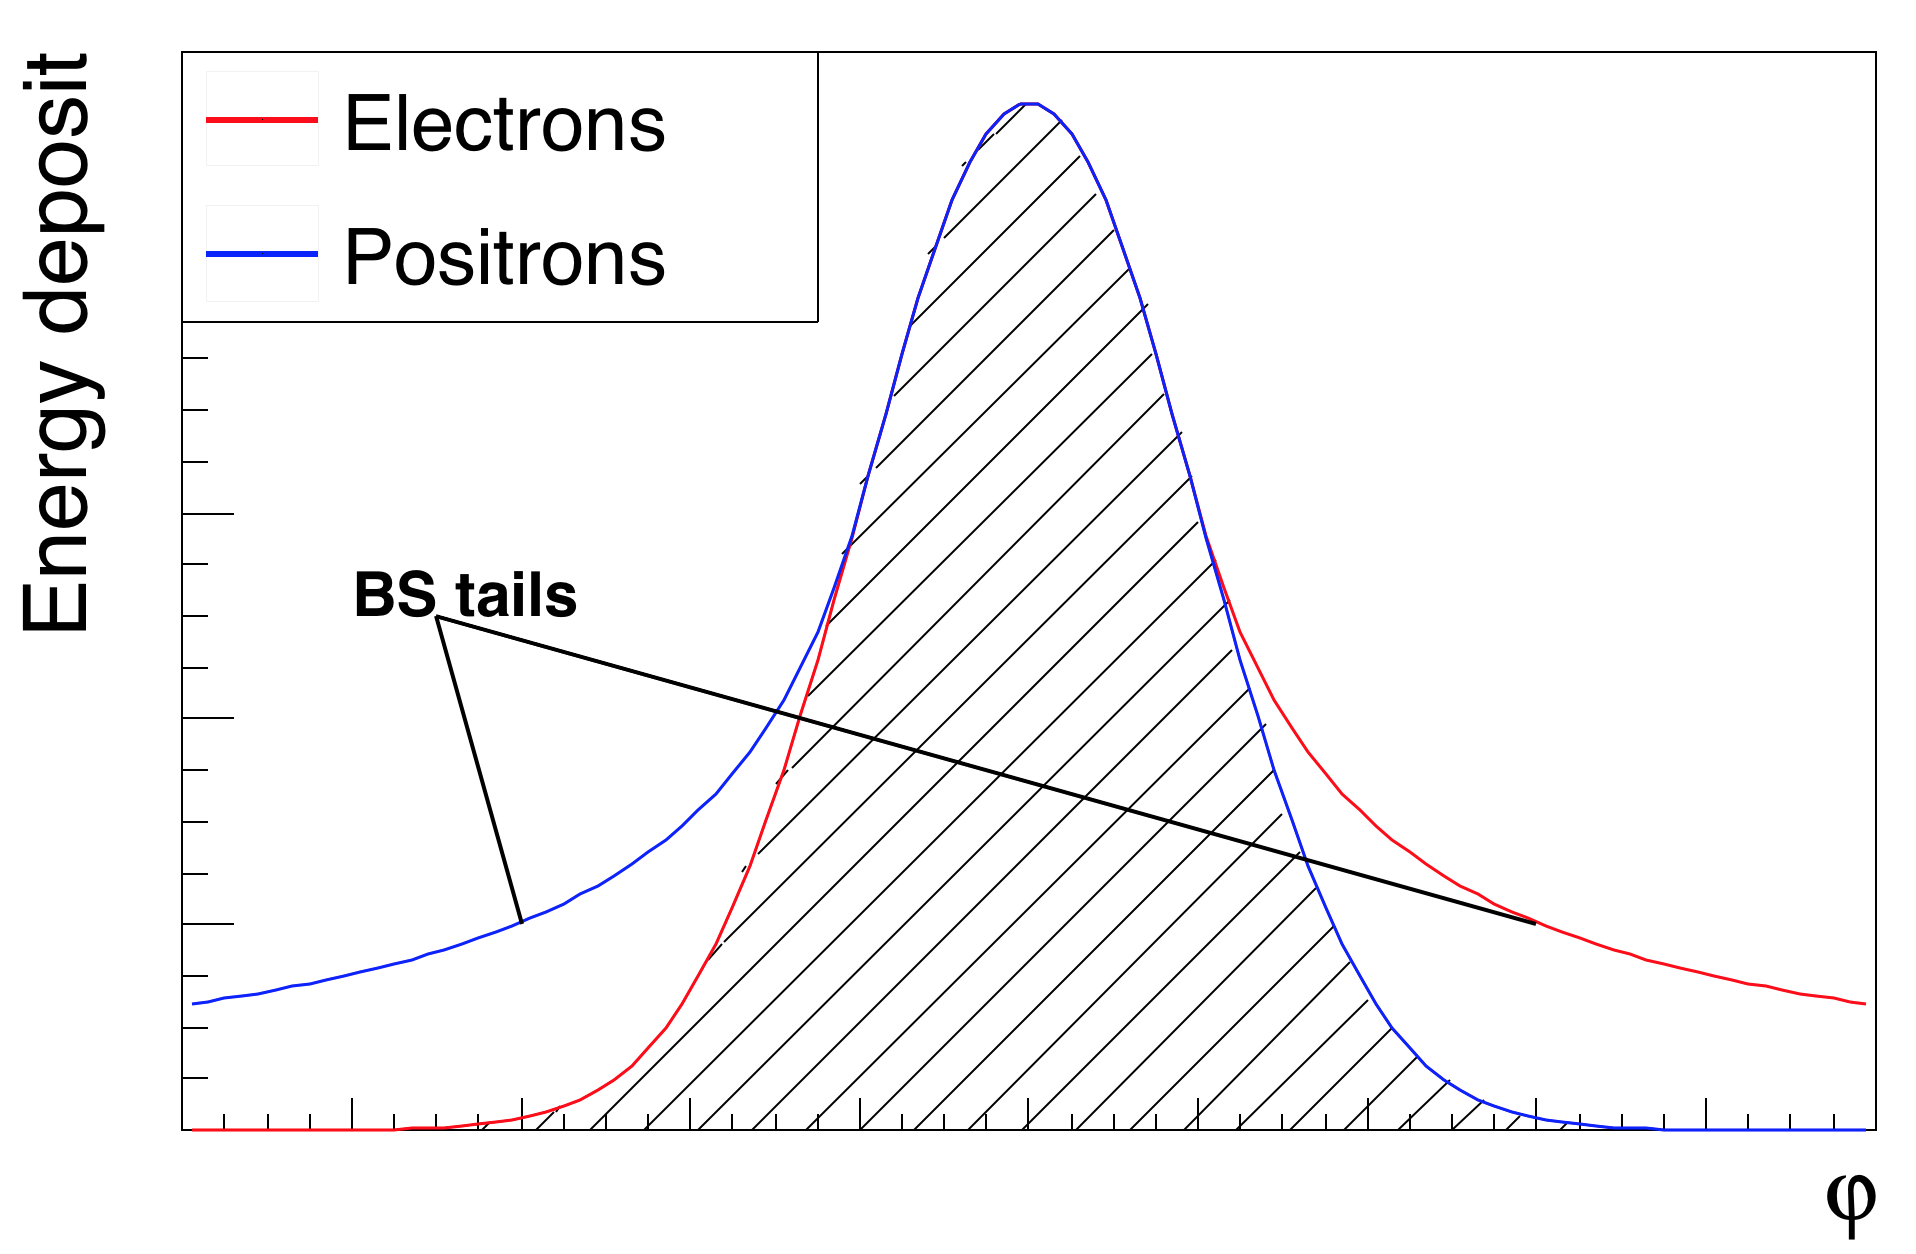
\includegraphics[width=10cm,height=7cm]{bs_tails.png}\\
The idea is to factor out material effects (we don't want to reweight Bremsstrahlung tails) and obtain same reweighting function for e+ and e- . For the reweighting function we would use only the hatched region.
\end{frame}

%------------------------------------------------

%------------------------------------------------
\begin{frame}
\frametitle{Reweighting function with Bremsstrahlung subtraction}
\begin{itemize}
\item We would like to have the same reweighting function for both $e^+$ and $e^-$. 
\item Let's extract the Bremsstrahlung-independent energy profile from the separated $e^+$ and $e^-$ energy profiles:
\end{itemize}
\begin{equation}
\nonumber
   \large {E_{i}^{Universal}} = \begin{cases}
{E_{i}^{Electron}}\text{, if }E_{i}^{Electron} < E_{i}^{Positron}\\
{E_{i}^{Positron}}\text{, if } E_{i}^{Electron} > E_{i}^{Positron}\\
\end{cases}
\text{, where } i = 1..77.
\end{equation}
\begin{itemize}

\end{itemize}
\item And now extract the Bremsstrahlung-independent reweighting function:
\begin{equation}
\nonumber
   \large {M_{i}^{Correction} = \frac{E_{i}^{Data}}{\Sigma E^{Data}} - \frac{E_{i}^{MC}}{\Sigma E^{MC}}}
\end{equation}
\end{frame}
%------------------------------------------------
%------------------------------------------------
\begin{frame}
\frametitle{Reweighted Bremsstrahlung-free $\eta$ energy profile and $R_\eta$, $\eta \in (1.8, 2.0)$}

\begin{columns}[t]
\column{.5\textwidth}
\centering
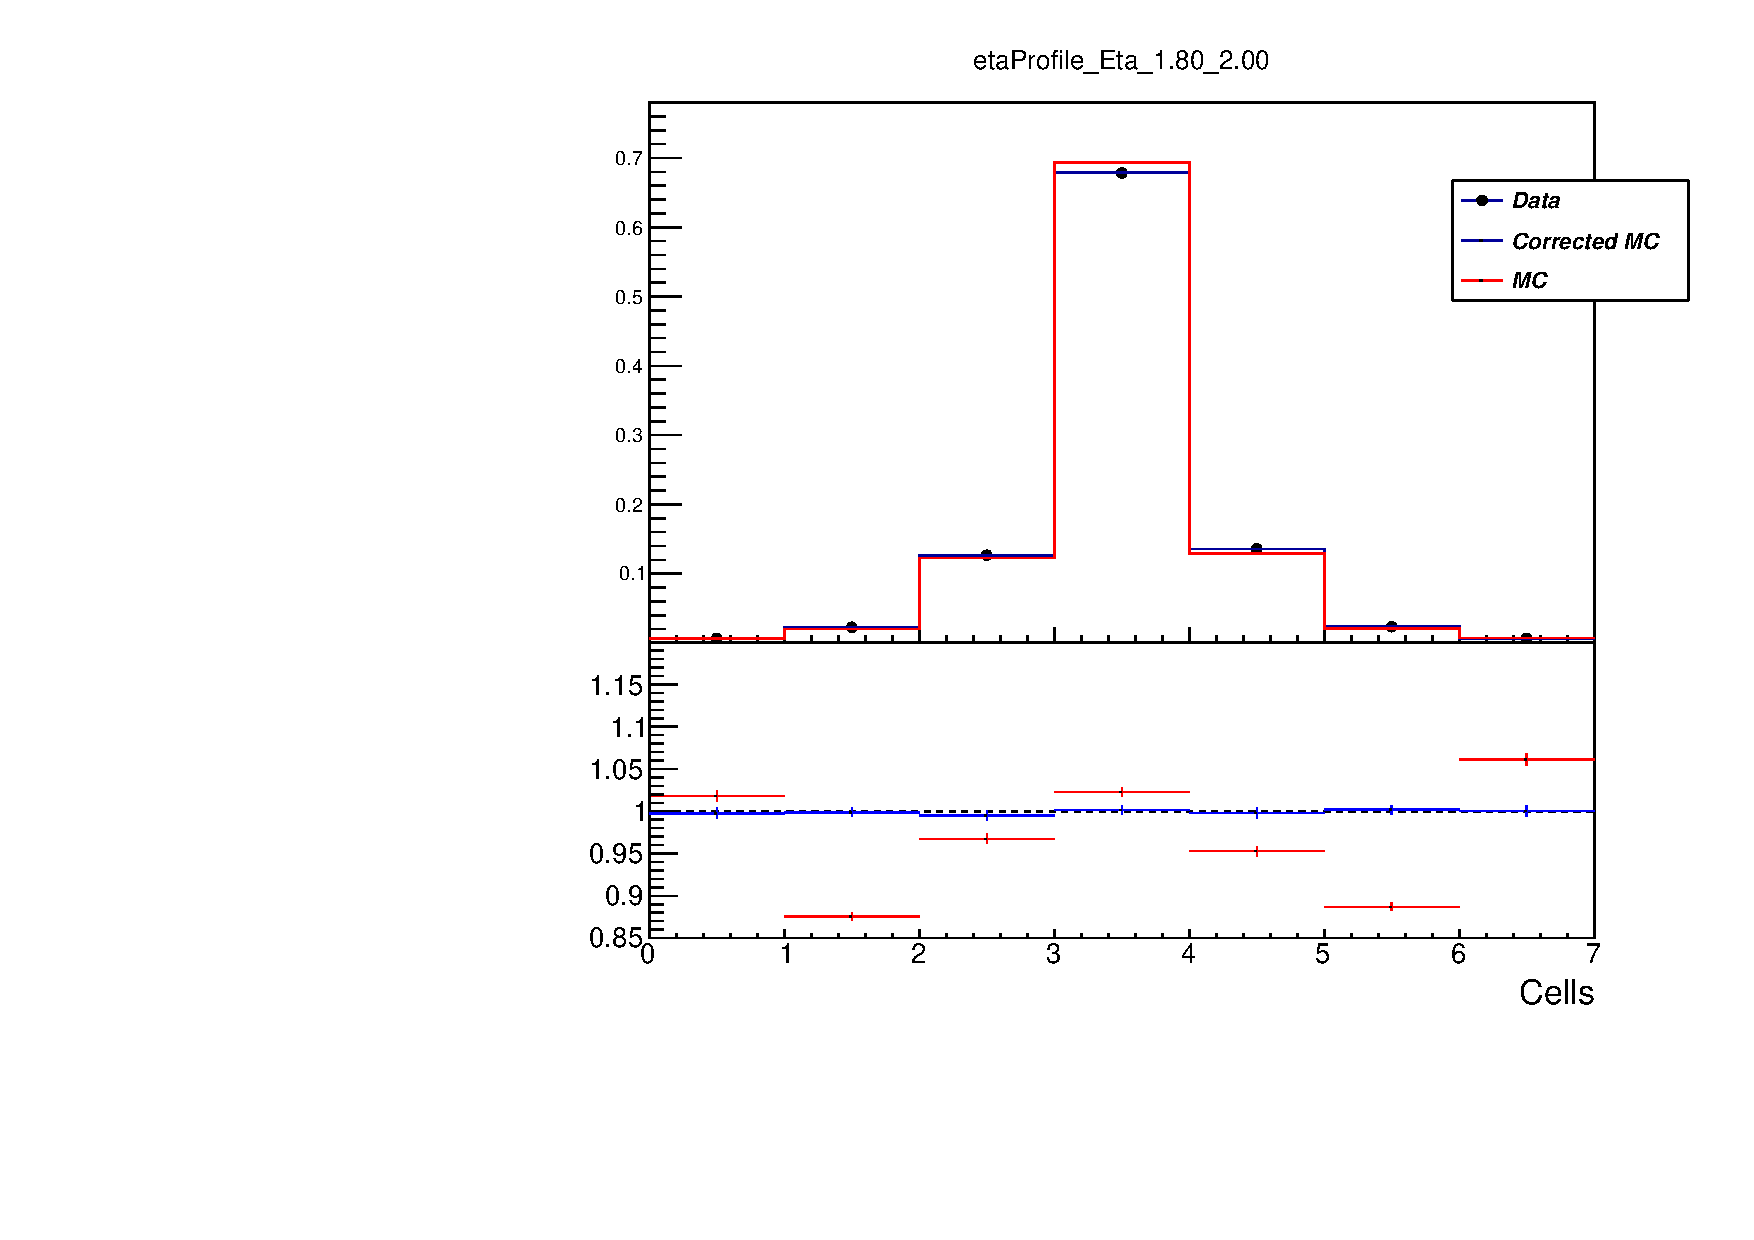
\includegraphics[width=6cm]{etaProfile_Rew_Eta_18_20_Local_Rew_noBS.pdf}
\column{.5\textwidth}
\centering
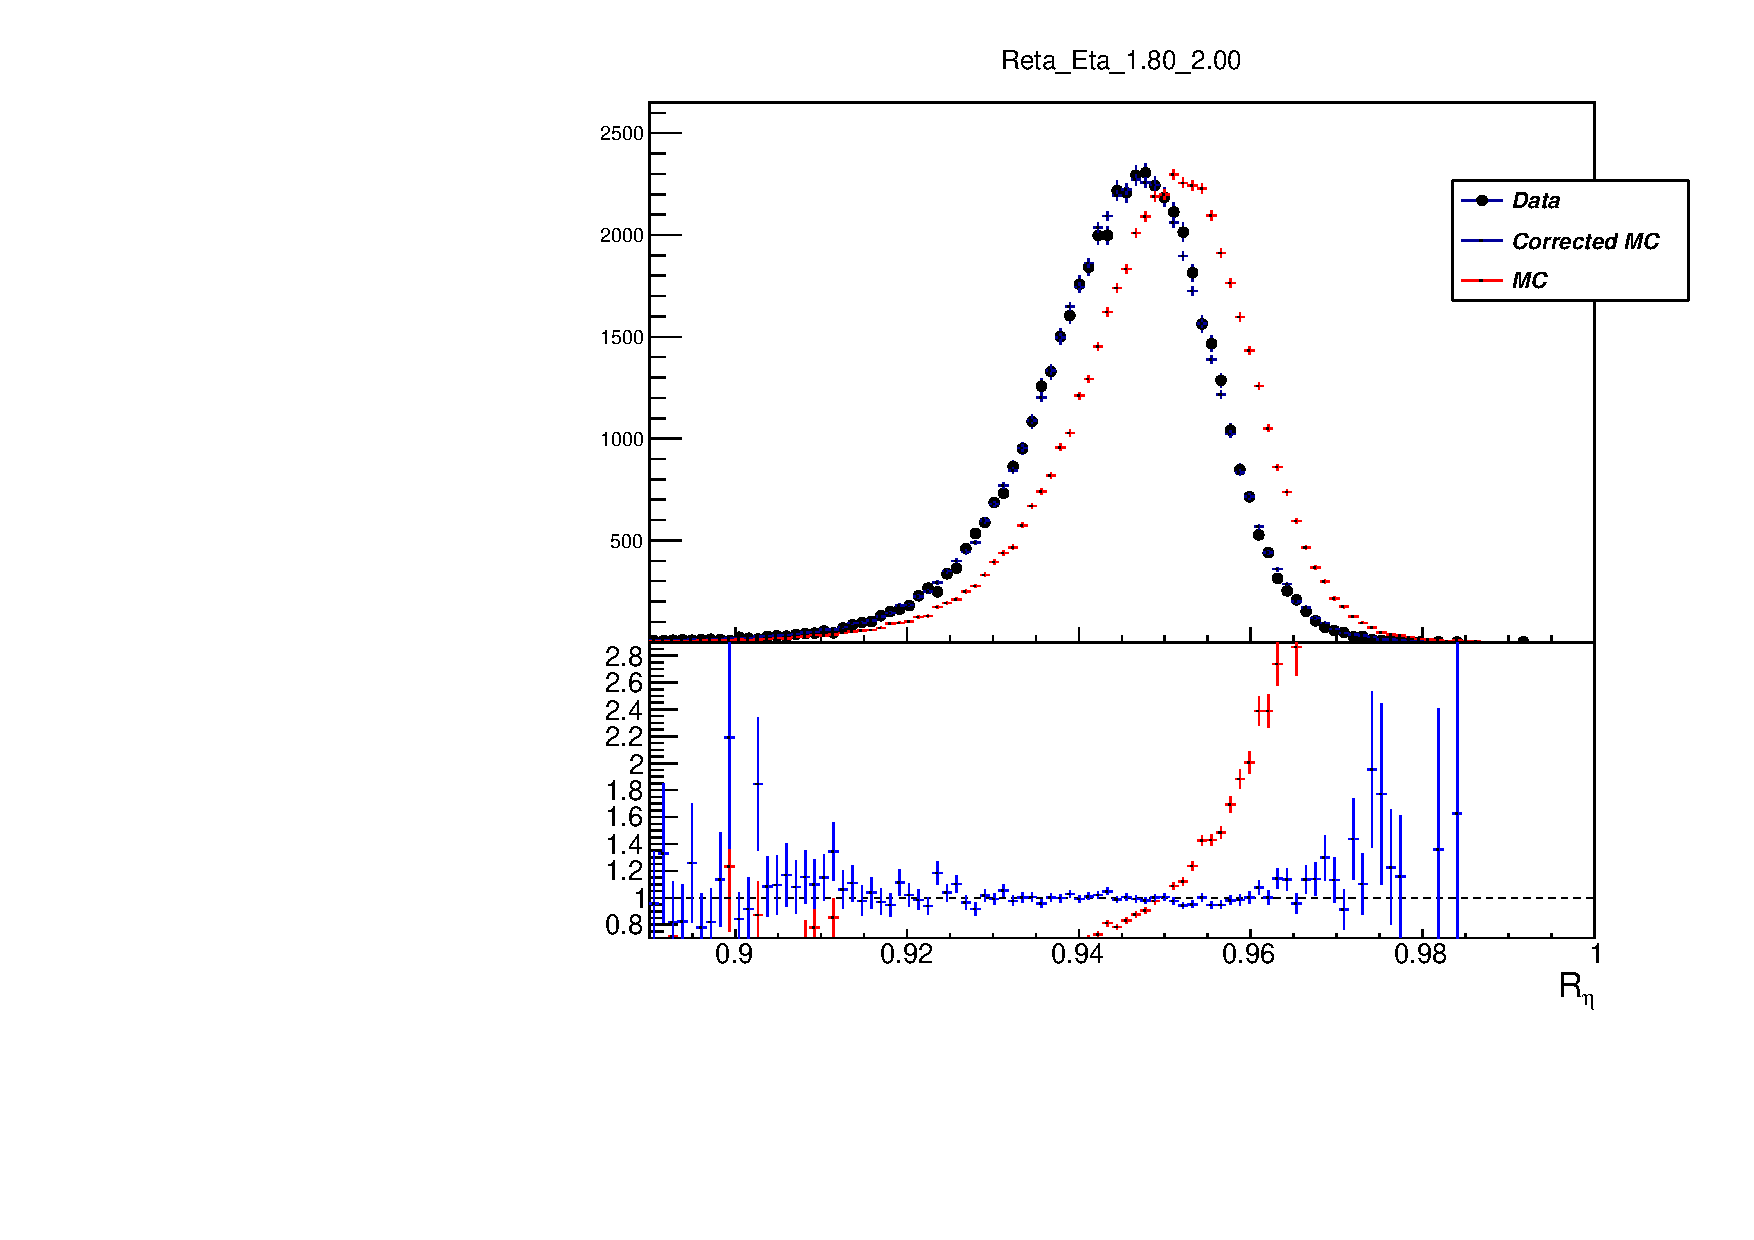
\includegraphics[width=6cm]{Reta_Rew_Eta_18_20_Local_Rew_noBS.pdf}
\end{columns}
\end{frame}
%------------------------------------------------
%------------------------------------------------
\begin{frame}
\frametitle{Reweighted Bremsstrahlung-free $\phi$ energy profile and $R_\phi$, $\eta \in (0.4, 0.6)$}

\begin{columns}[t]
\column{.5\textwidth}
\centering
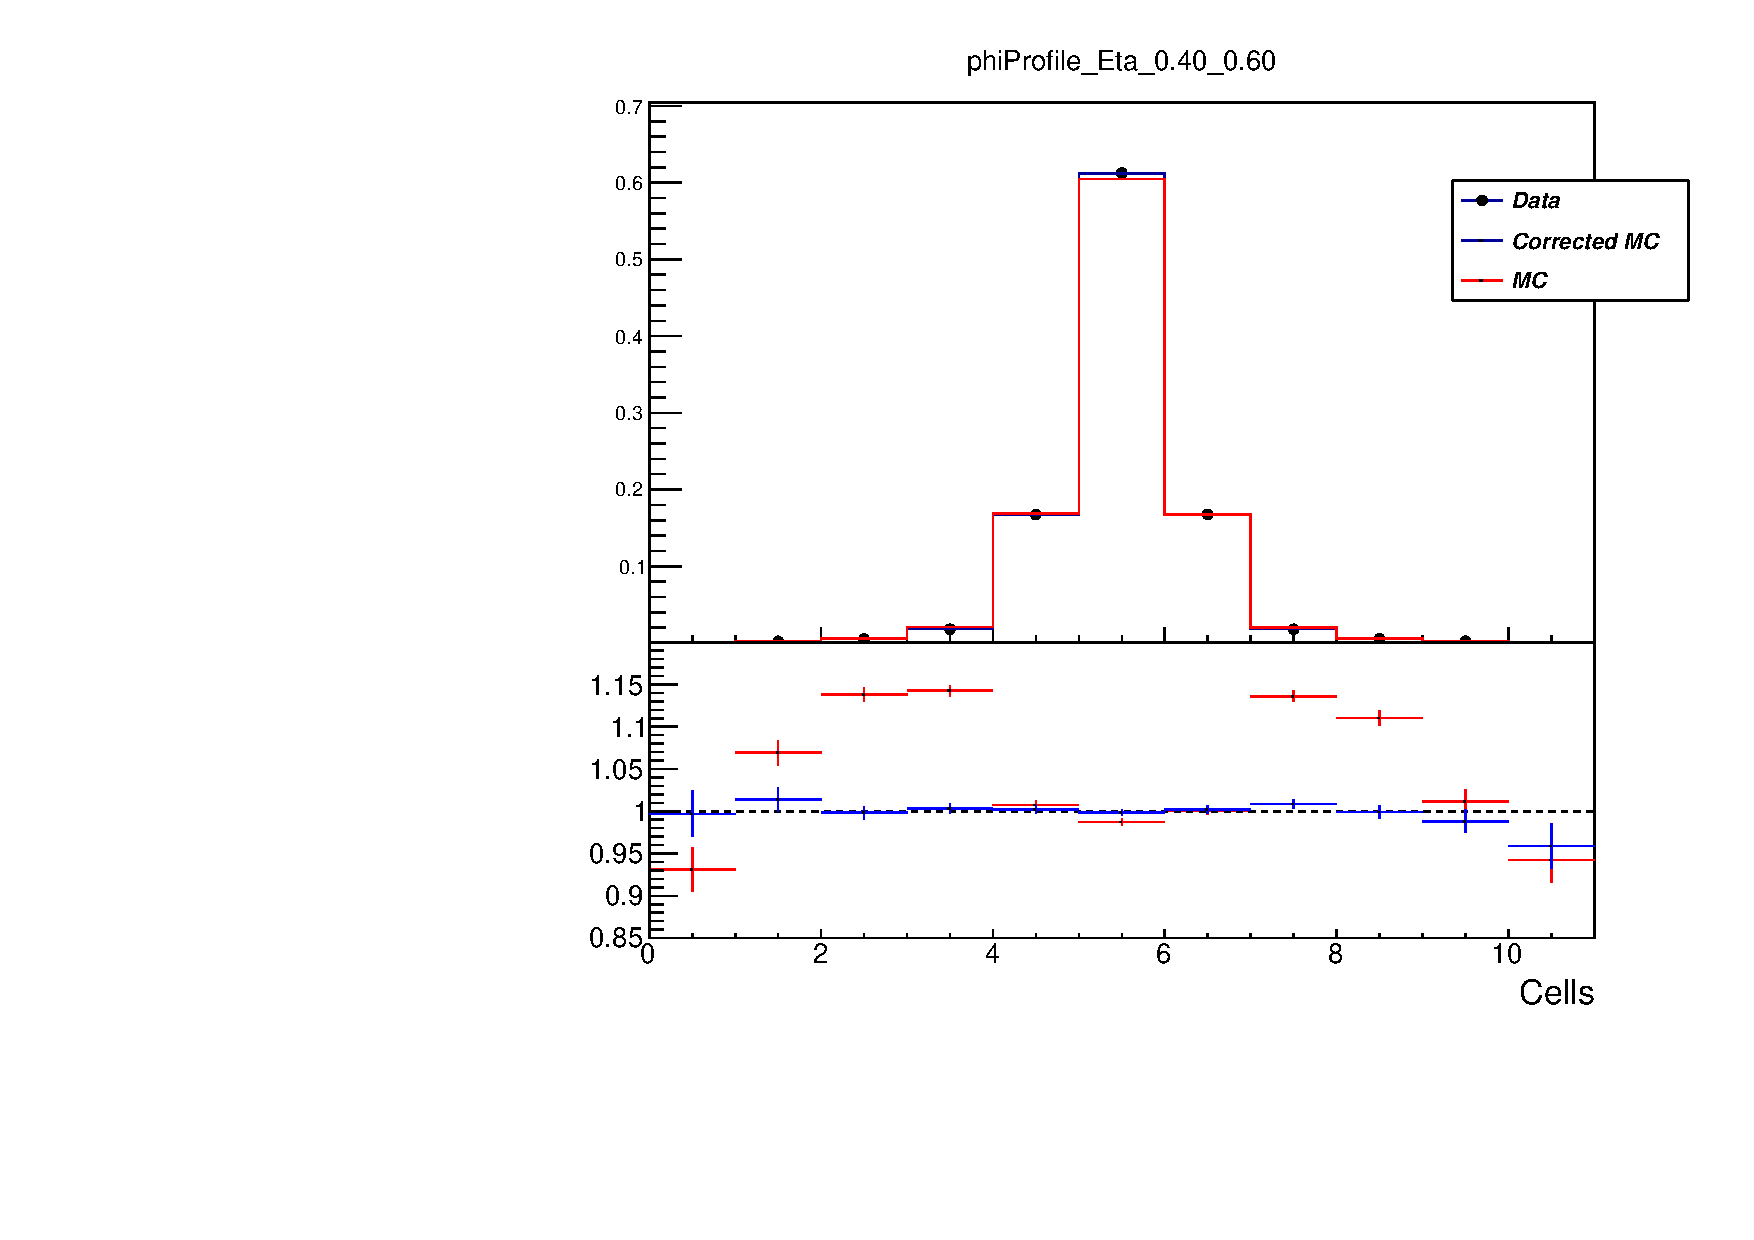
\includegraphics[width=6cm]{phiProfile_Rew_Eta_4_6_Local_Rew_noBS.pdf}\\
\column{.5\textwidth}
\centering
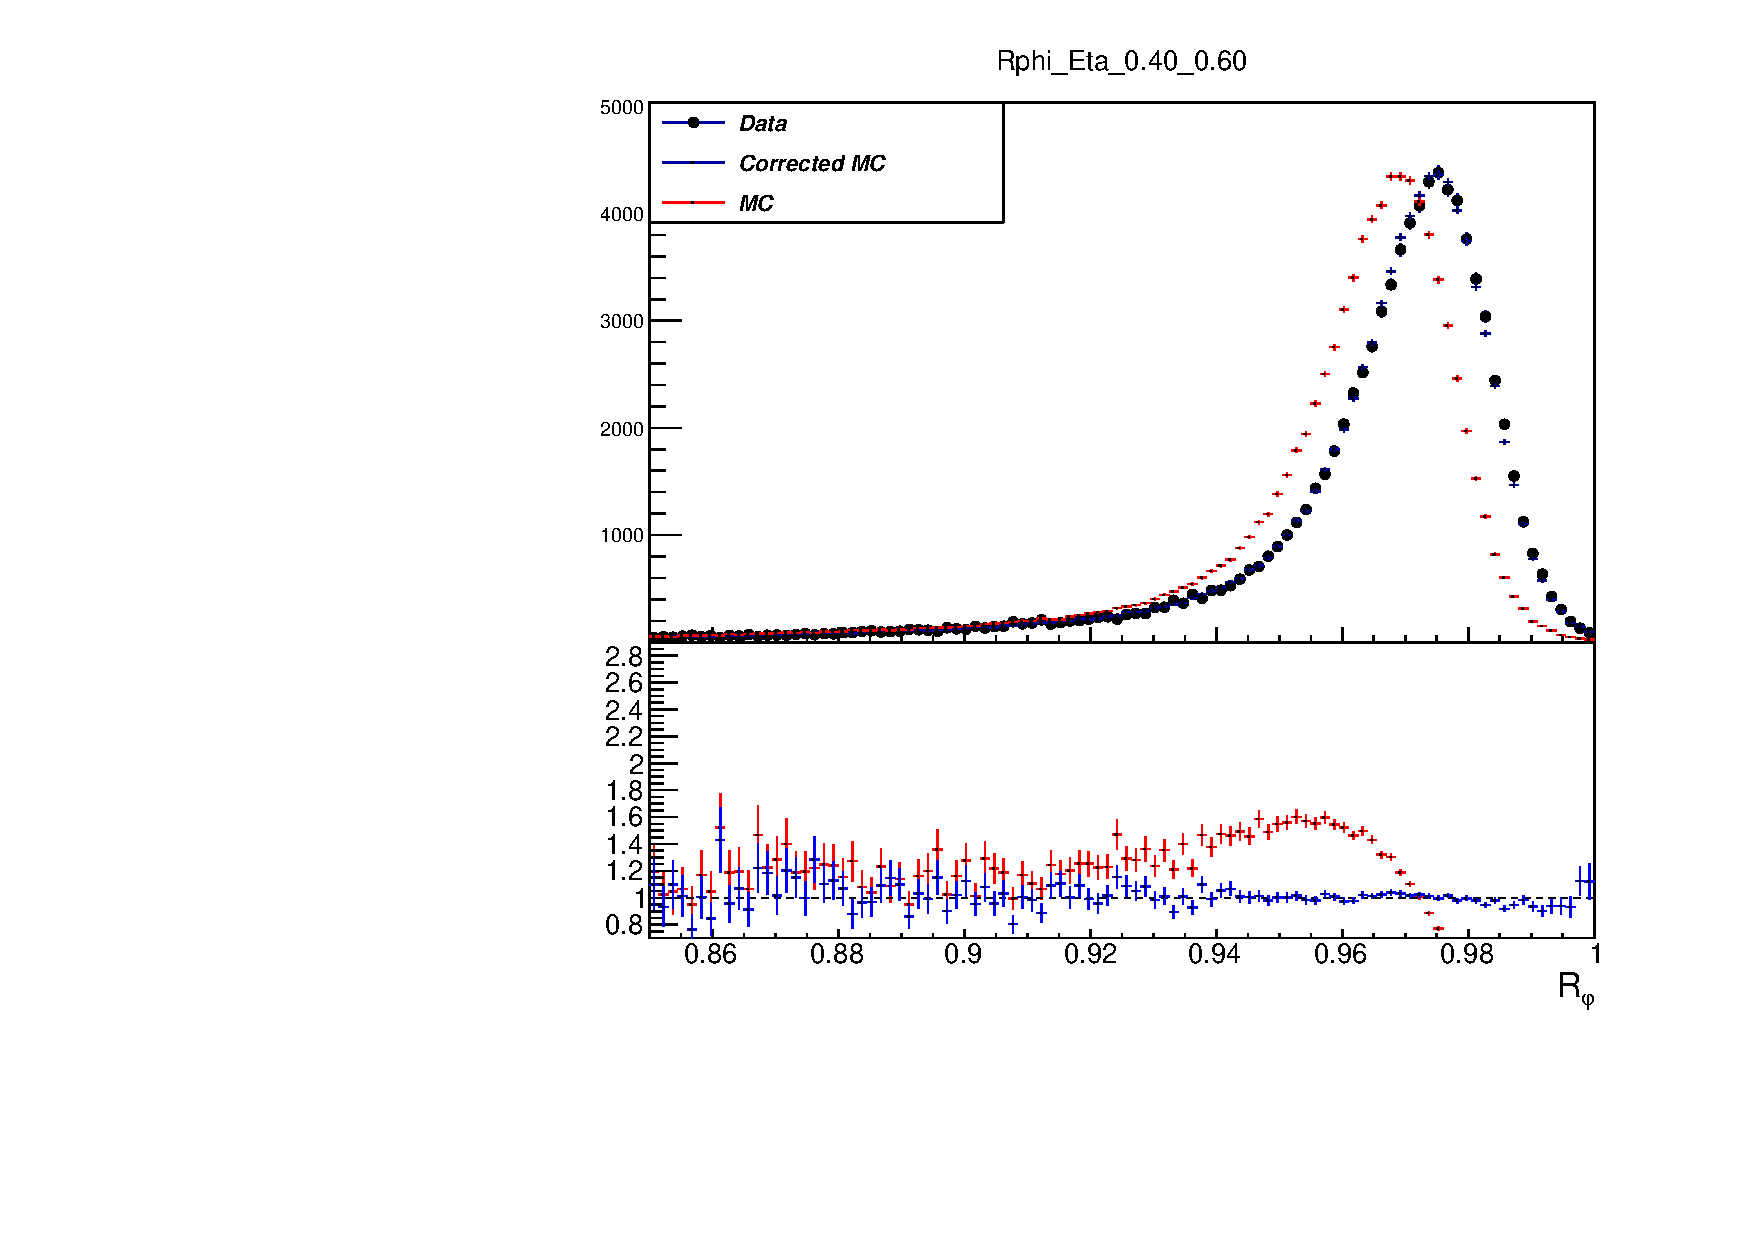
\includegraphics[width=6cm]{Rphi_Rew_Eta_4_6_Local_Rew_noBS.pdf}\\

\end{columns}
\end{frame}
%------------------------------------------------

%------------------------------------------------
\begin{frame}
\frametitle{Reweighting steps}
\begin{itemize}
\item Local closure test \textcolor{red}{ $\checkmark$}\\
\item Local test for Bremsstrahlung subtraction \textcolor{red}{ $\checkmark$}\\

\end{itemize}
\end{frame}
%------------------------------------------------
%------------------------------------------------
\begin{frame}
\frametitle{Technicalities - Athena implementation}
Cell reweighting is an option included within the DerivationFrameworkCalo package. 
\begin{itemize}
\item CellReweight tool, previously developed to do the 1D reweighting in Eta is now doing 2D (eta and phi) reweighting in the second layer of the calorimeter. Reads the 2D reweighting coefficients, stored in .root file. A temporary cell container is created for the reweighted cells.
\item ClusterEnergyPerLayerDecorator - links the electron container to the new cells.
\item ElectronReweight - creates an extra electron container with new shower shapes.
\item For the purposes of systematics study we've included an option to use 3 different reweighting functions creating 3 electron containers with reweighting variations.

\end{itemize}
\end{frame}

%------------------------------------------------
%------------------------------------------------
\begin{frame}
\frametitle{Athena implementation challenges}
\begin{itemize}
\item Egamma cluster contains links to a set of cells with no information on their relative position.
\item \textcolor{red}{Problem 1:} In order to do the reweighting we need to know precisely the relative position of every cell in the 7x11 cluster.
\item A big fraction (about 40\%) of electron clusters are not complete ($N_{cells} \ne 77$) lacking peripheral cells.
\item \textcolor{red}{Problem 2:} an attempt to access a non-existing cell leads to Athena crash.
\end{itemize}
\end{frame}

%------------------------------------------------
%------------------------------------------------
\begin{frame}
\frametitle{Cluster sizes}

\centering
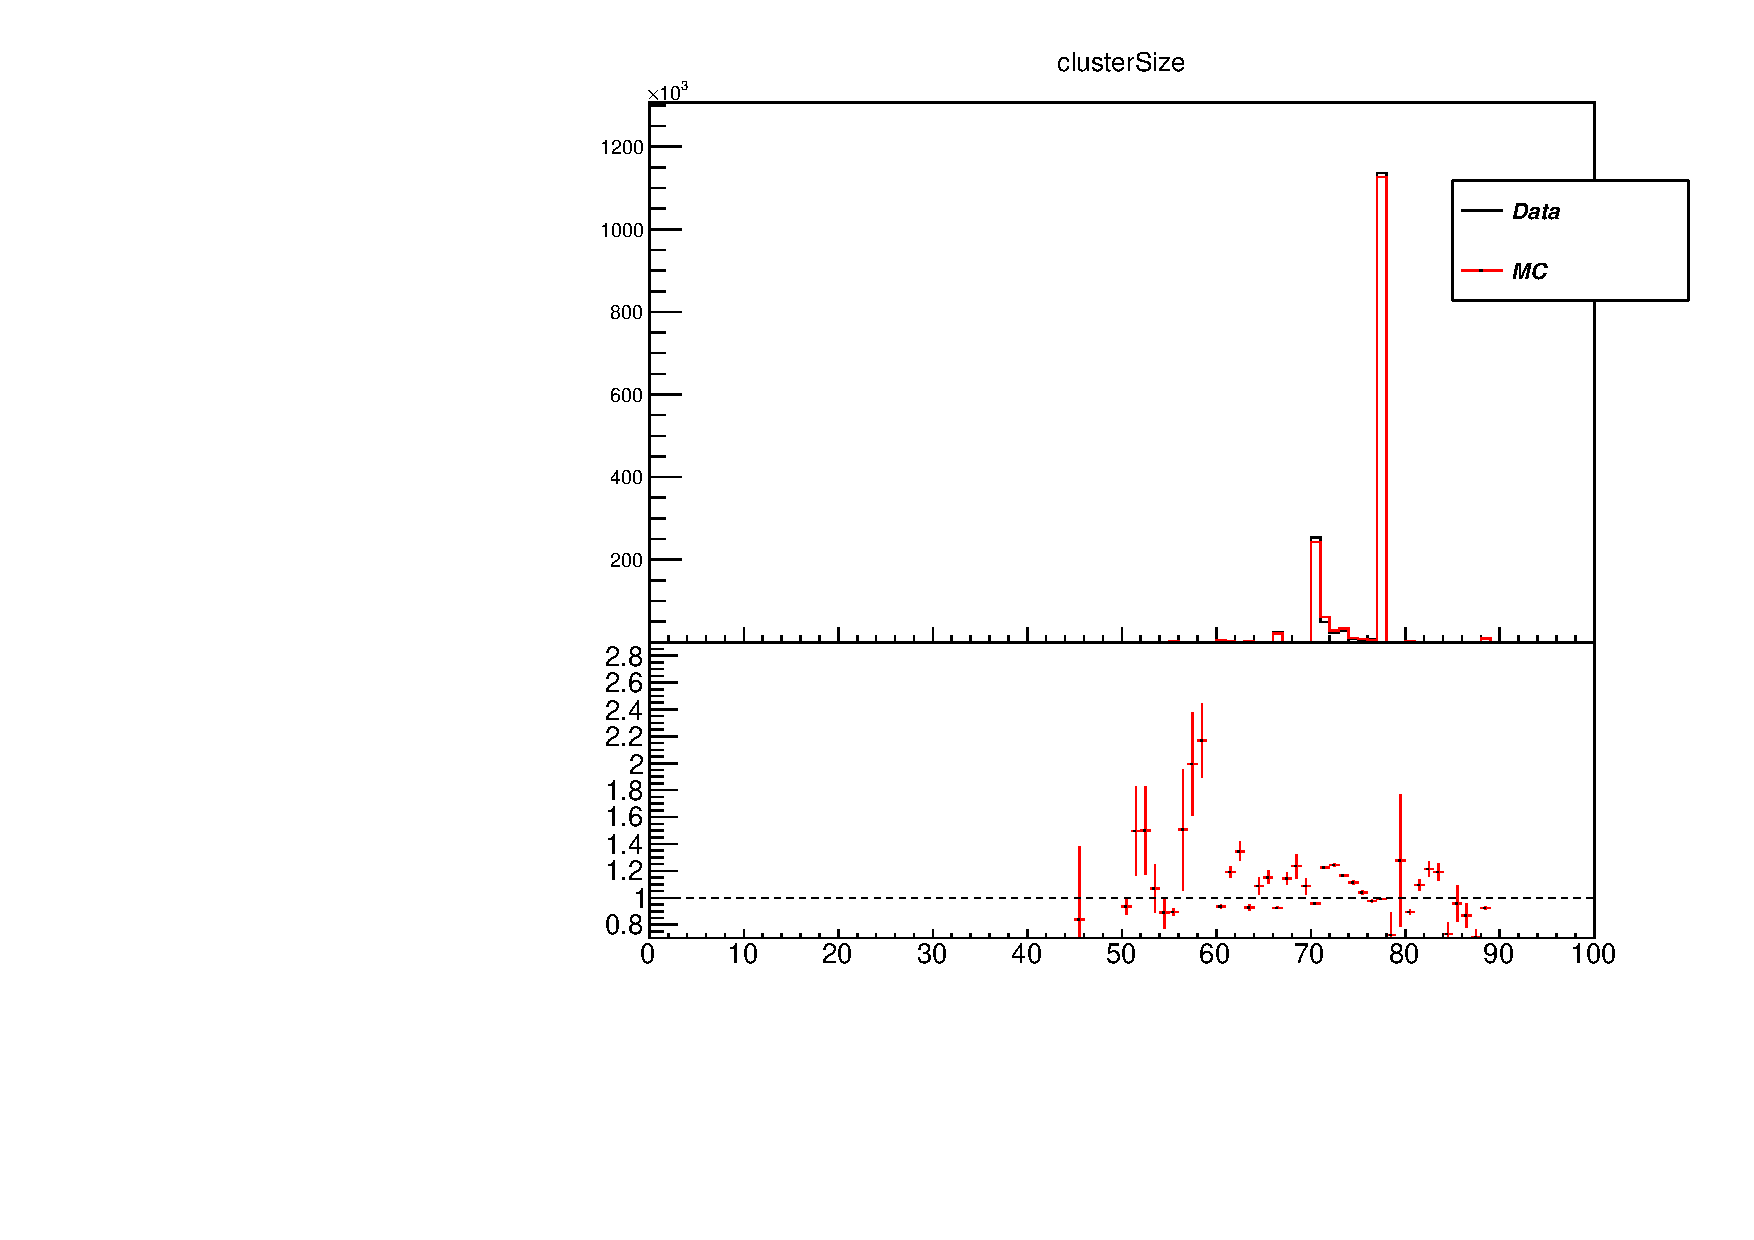
\includegraphics[height=8cm]{clusterSize.pdf}\\

\end{frame}
%------------------------------------------------
%------------------------------------------------
\begin{frame}
\frametitle{Schematic images of incomplete clusters}

\centering
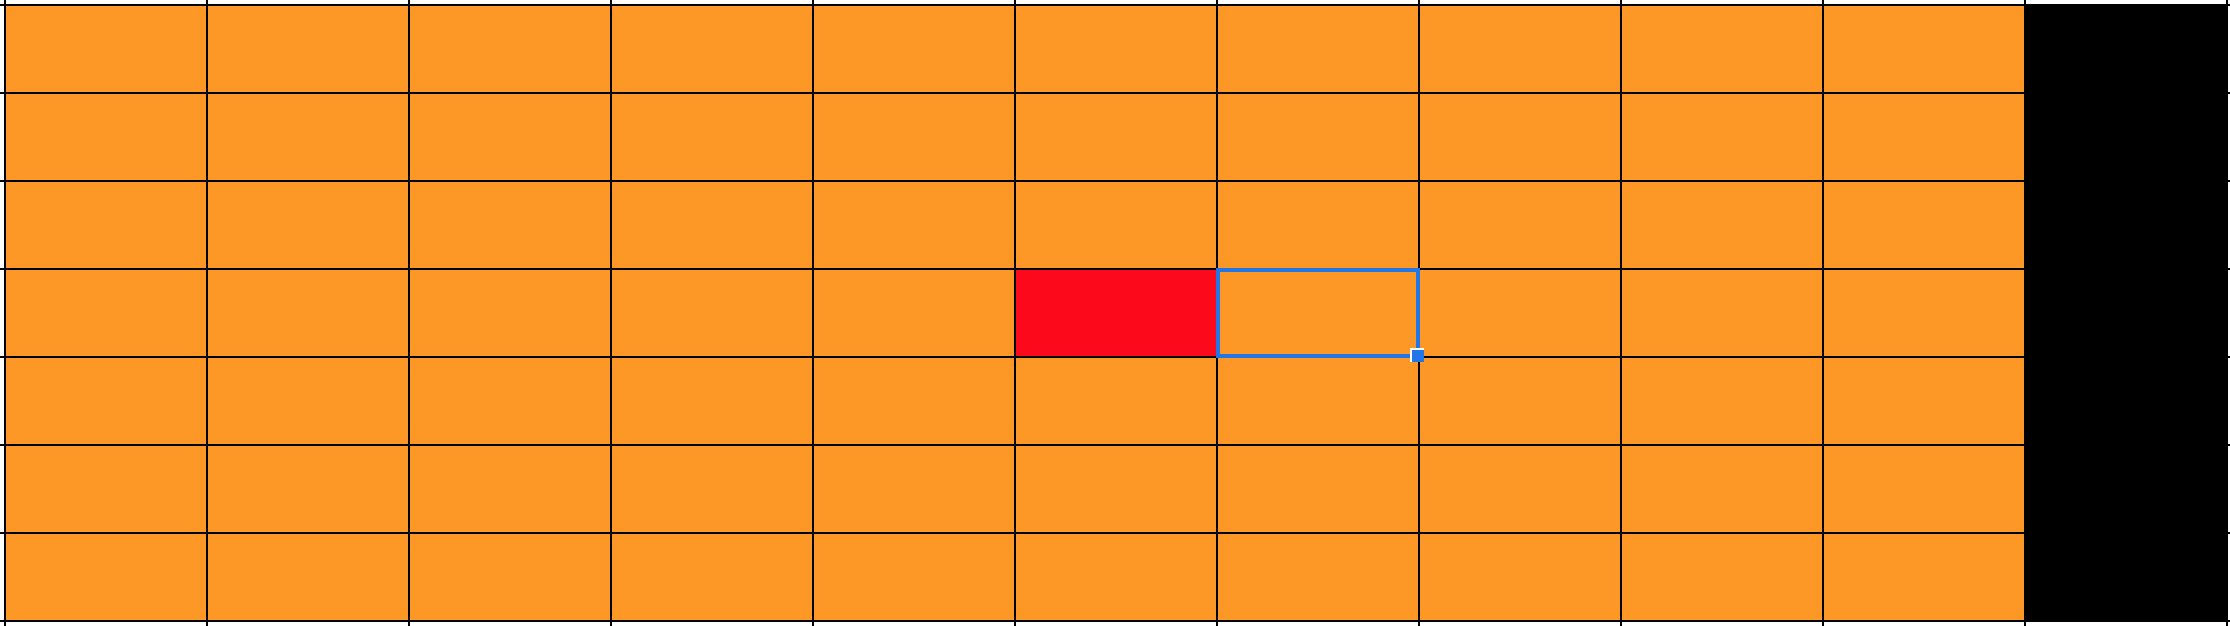
\includegraphics[width=10cm,height=2cm]{70_cells.png}\\
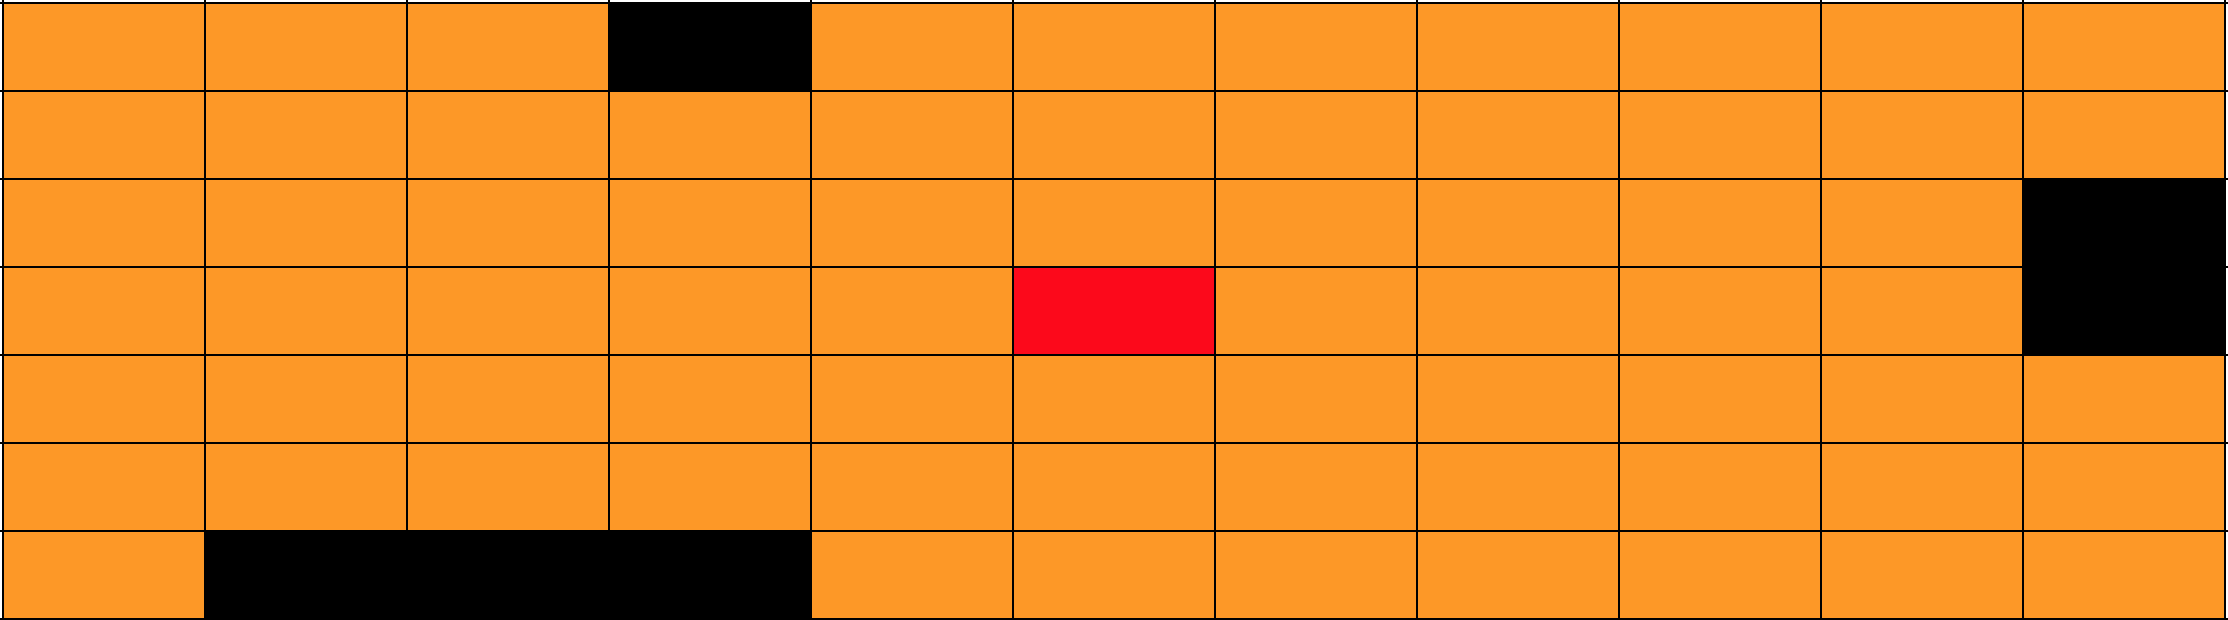
\includegraphics[width=10cm,height=2cm]{71_cells.png}\\
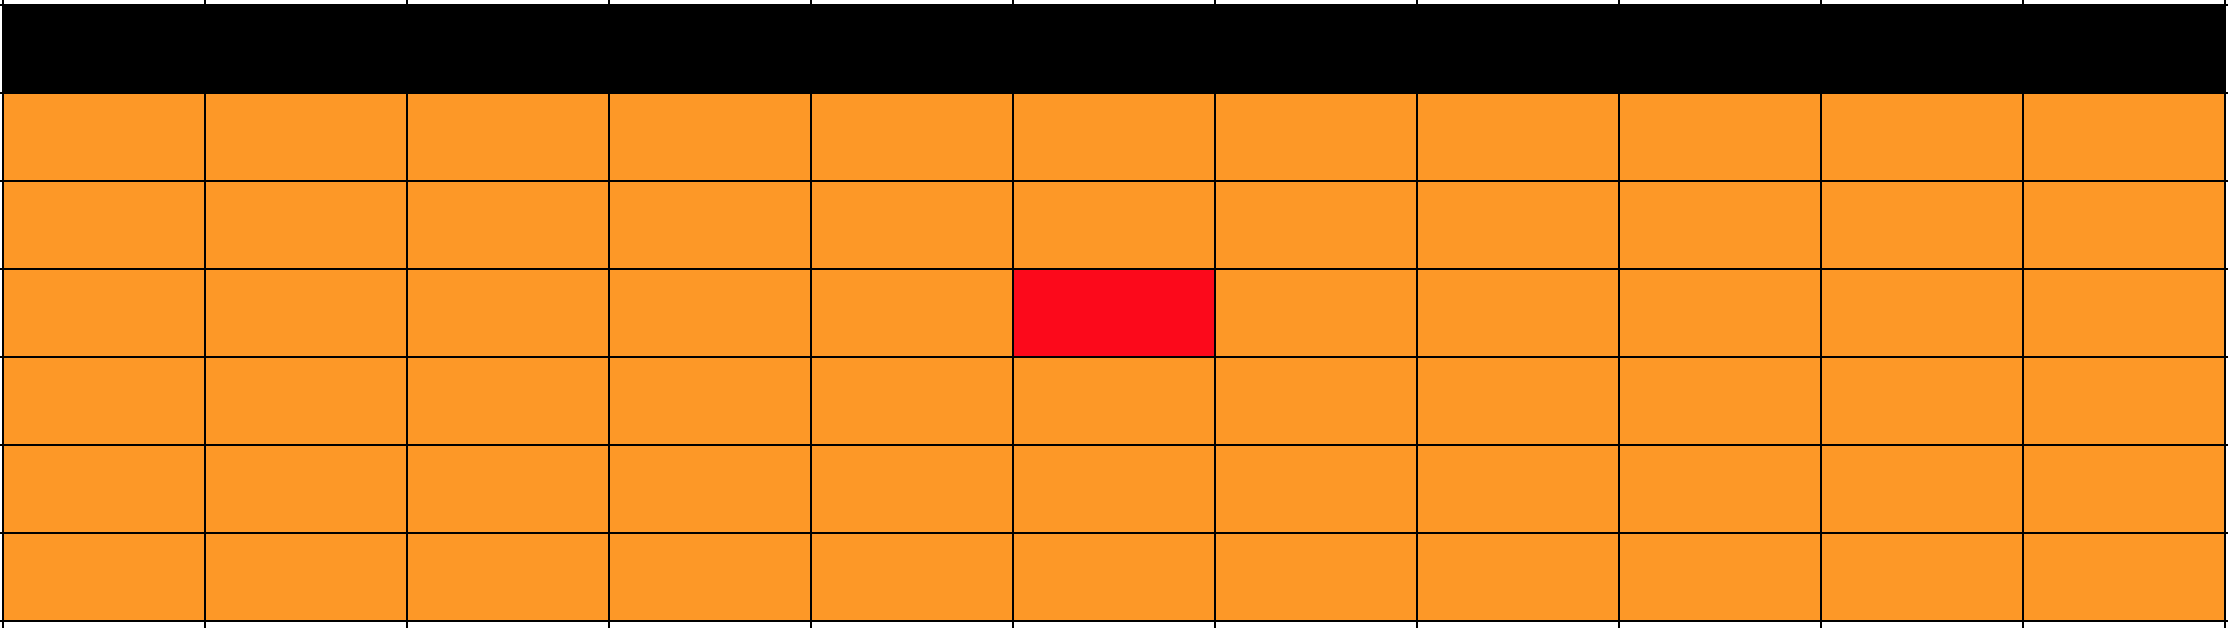
\includegraphics[width=10cm,height=2cm]{66_cells.png}\\
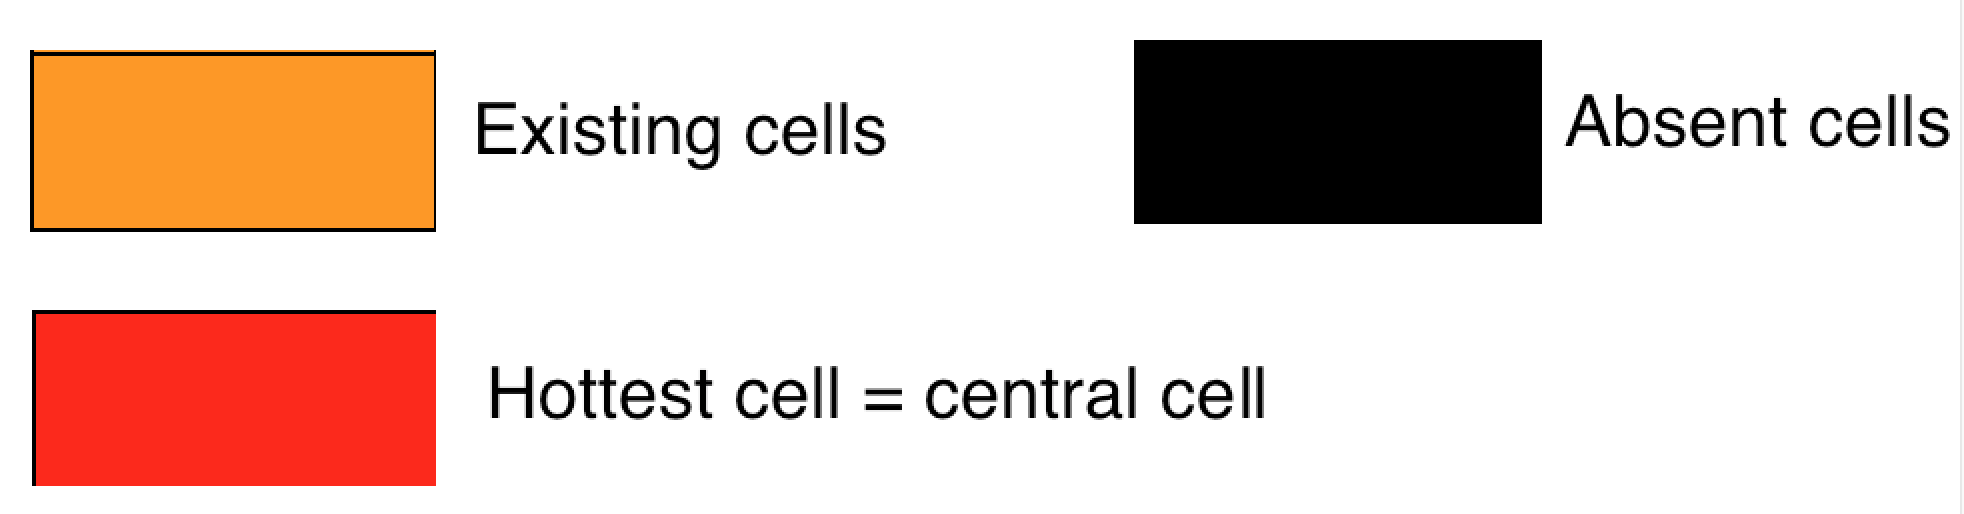
\includegraphics[width=6cm,height=2cm]{cells_legend.png}\\


\end{frame}
%------------------------------------------------
%------------------------------------------------
\begin{frame}
\frametitle{Reweighting steps}
\begin{itemize}
\item Local closure test \textcolor{red}{ $\checkmark$}\\
\item Local test for Bremsstrahlung subtraction \textcolor{red}{ $\checkmark$}\\
\item Athena closure test - reweighting complete clusters exclusively must be similar to local run with BS subtraction.\\
\end{itemize}
\end{frame}
%------------------------------------------------

%------------------------------------------------

\begin{frame}
\frametitle{Athena derivation reweighting (right) vs local test (left), $\eta$ profile, $\eta \in (1.8, 2.0)$, complete clusters only}

\begin{columns}[t]

\column{.5\textwidth}
\centering
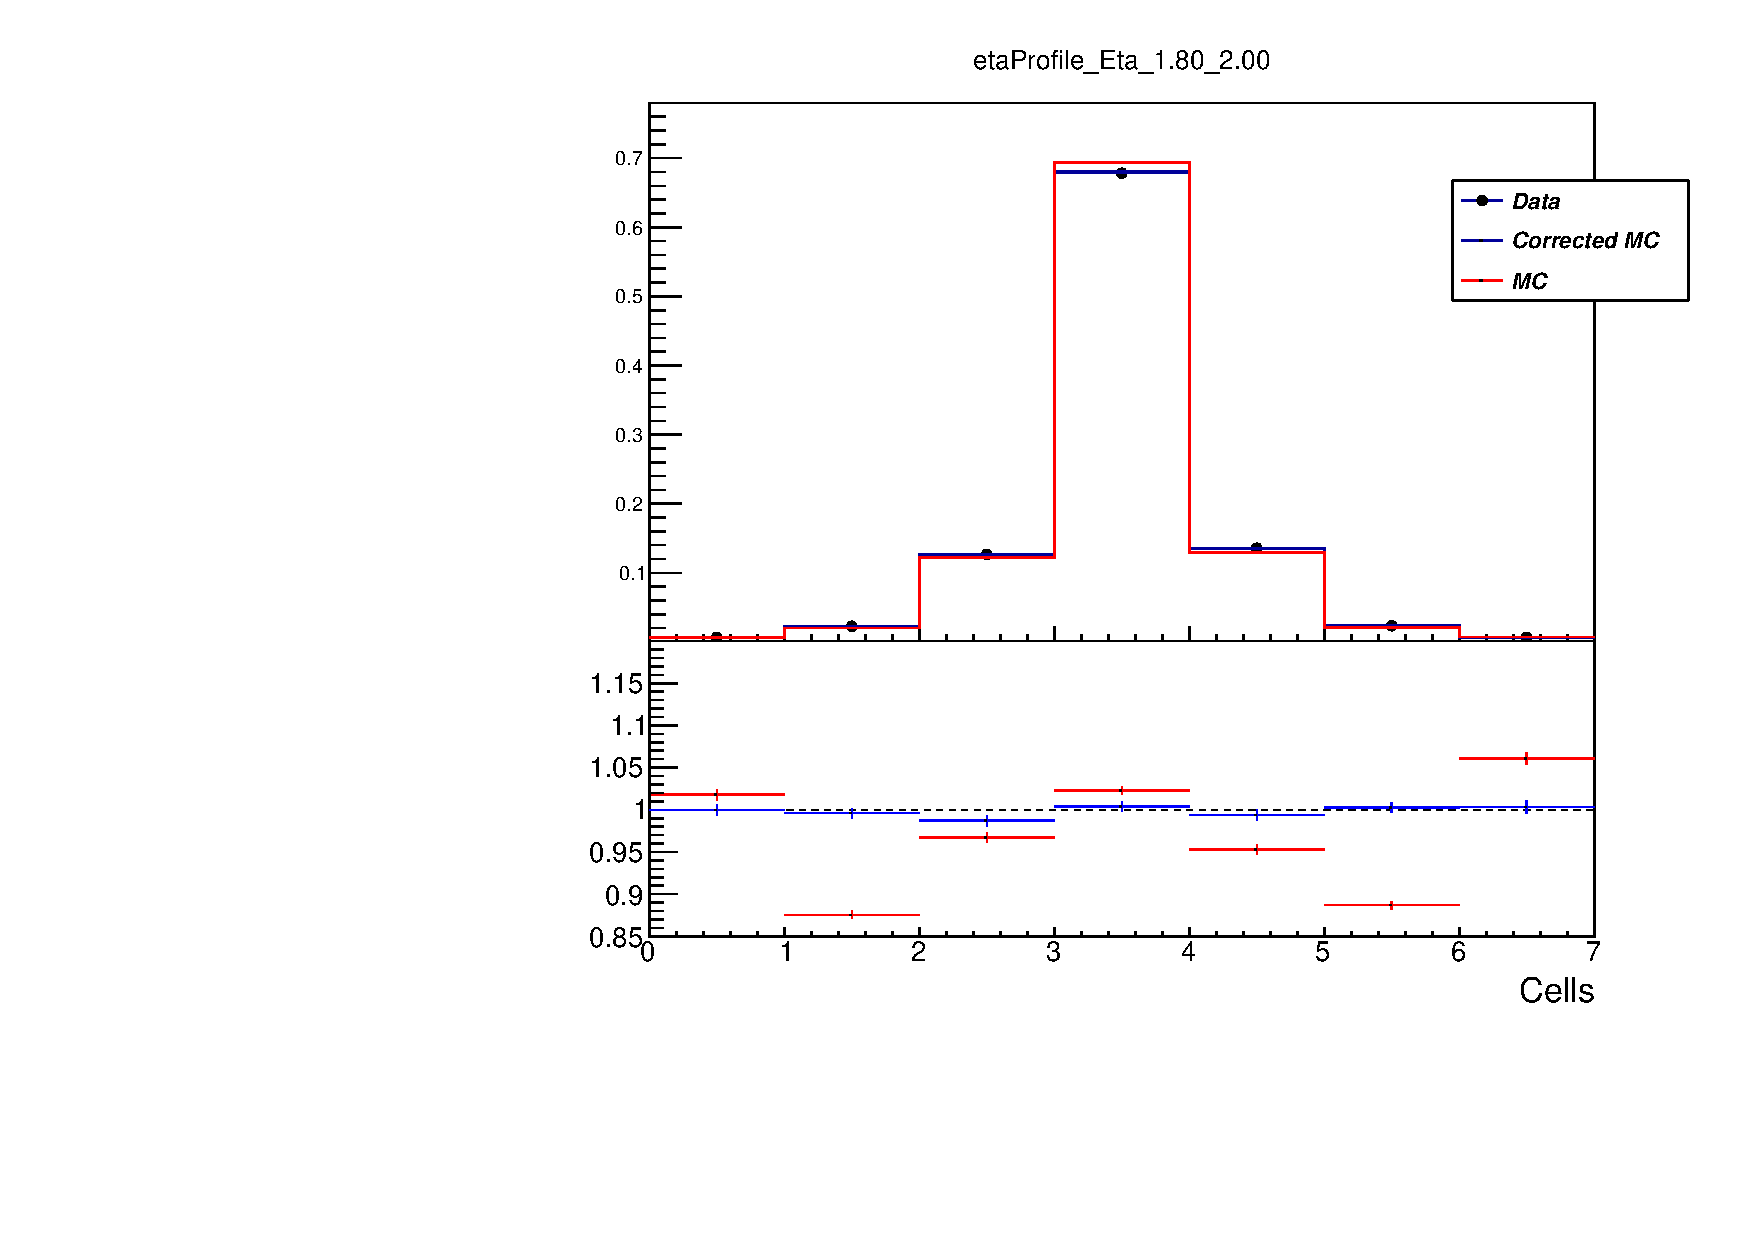
\includegraphics[width=6cm]{etaProfile_Eta_18_20_Athena.pdf}\\
\column{.5\textwidth}
\centering
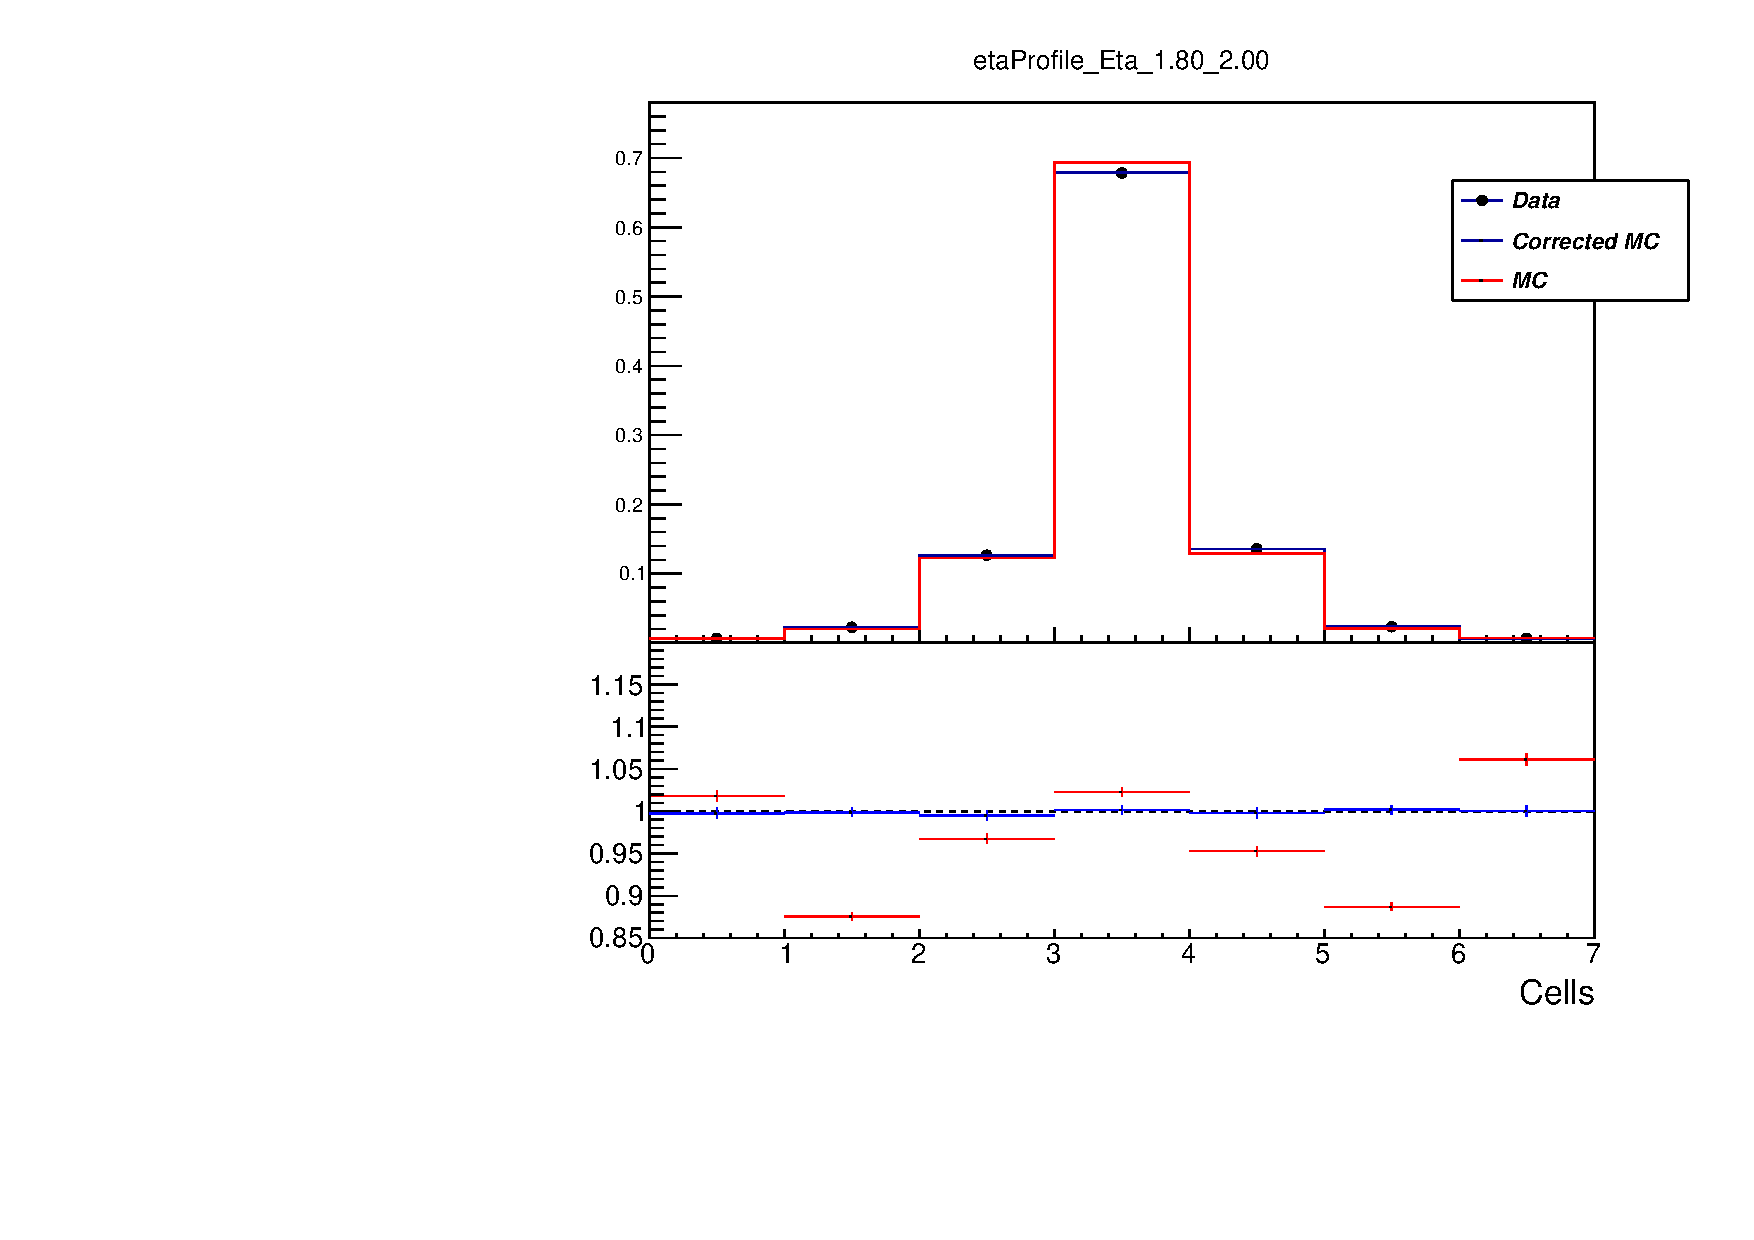
\includegraphics[width=6cm]{etaProfile_Rew_Eta_18_20_Local_Rew_noBS.pdf}\\
\end{columns}
\end{frame}
%------------------------------------------------
%------------------------------------------------

\begin{frame}
\frametitle{Athena derivation reweighting (right) vs local test (left), $\phi$ profile, $\eta \in (0.4, 0.6)$, complete clusters only}

\begin{columns}[t]

\column{.5\textwidth}
\centering
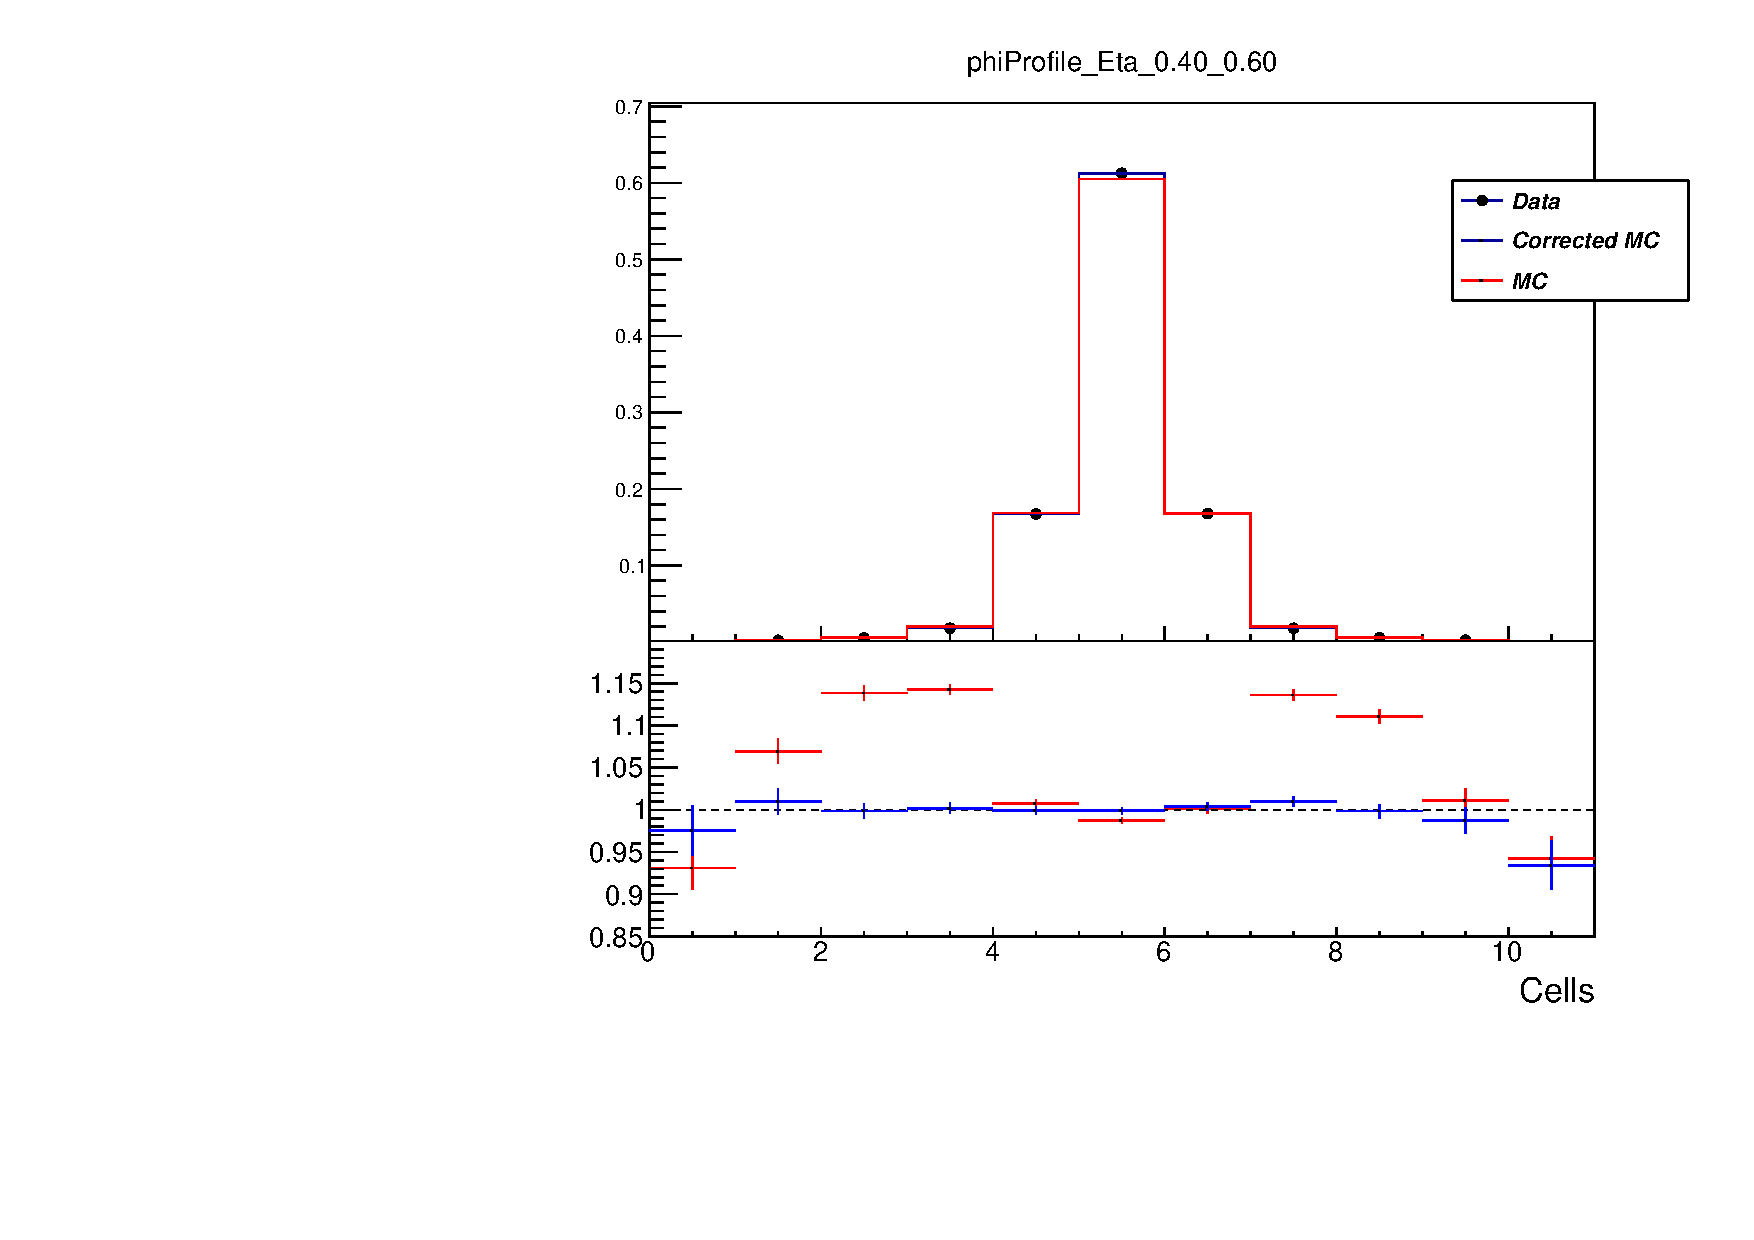
\includegraphics[width=6cm]{phiProfile_Eta_4_6_Athena.pdf}\\
\column{.5\textwidth}
\centering
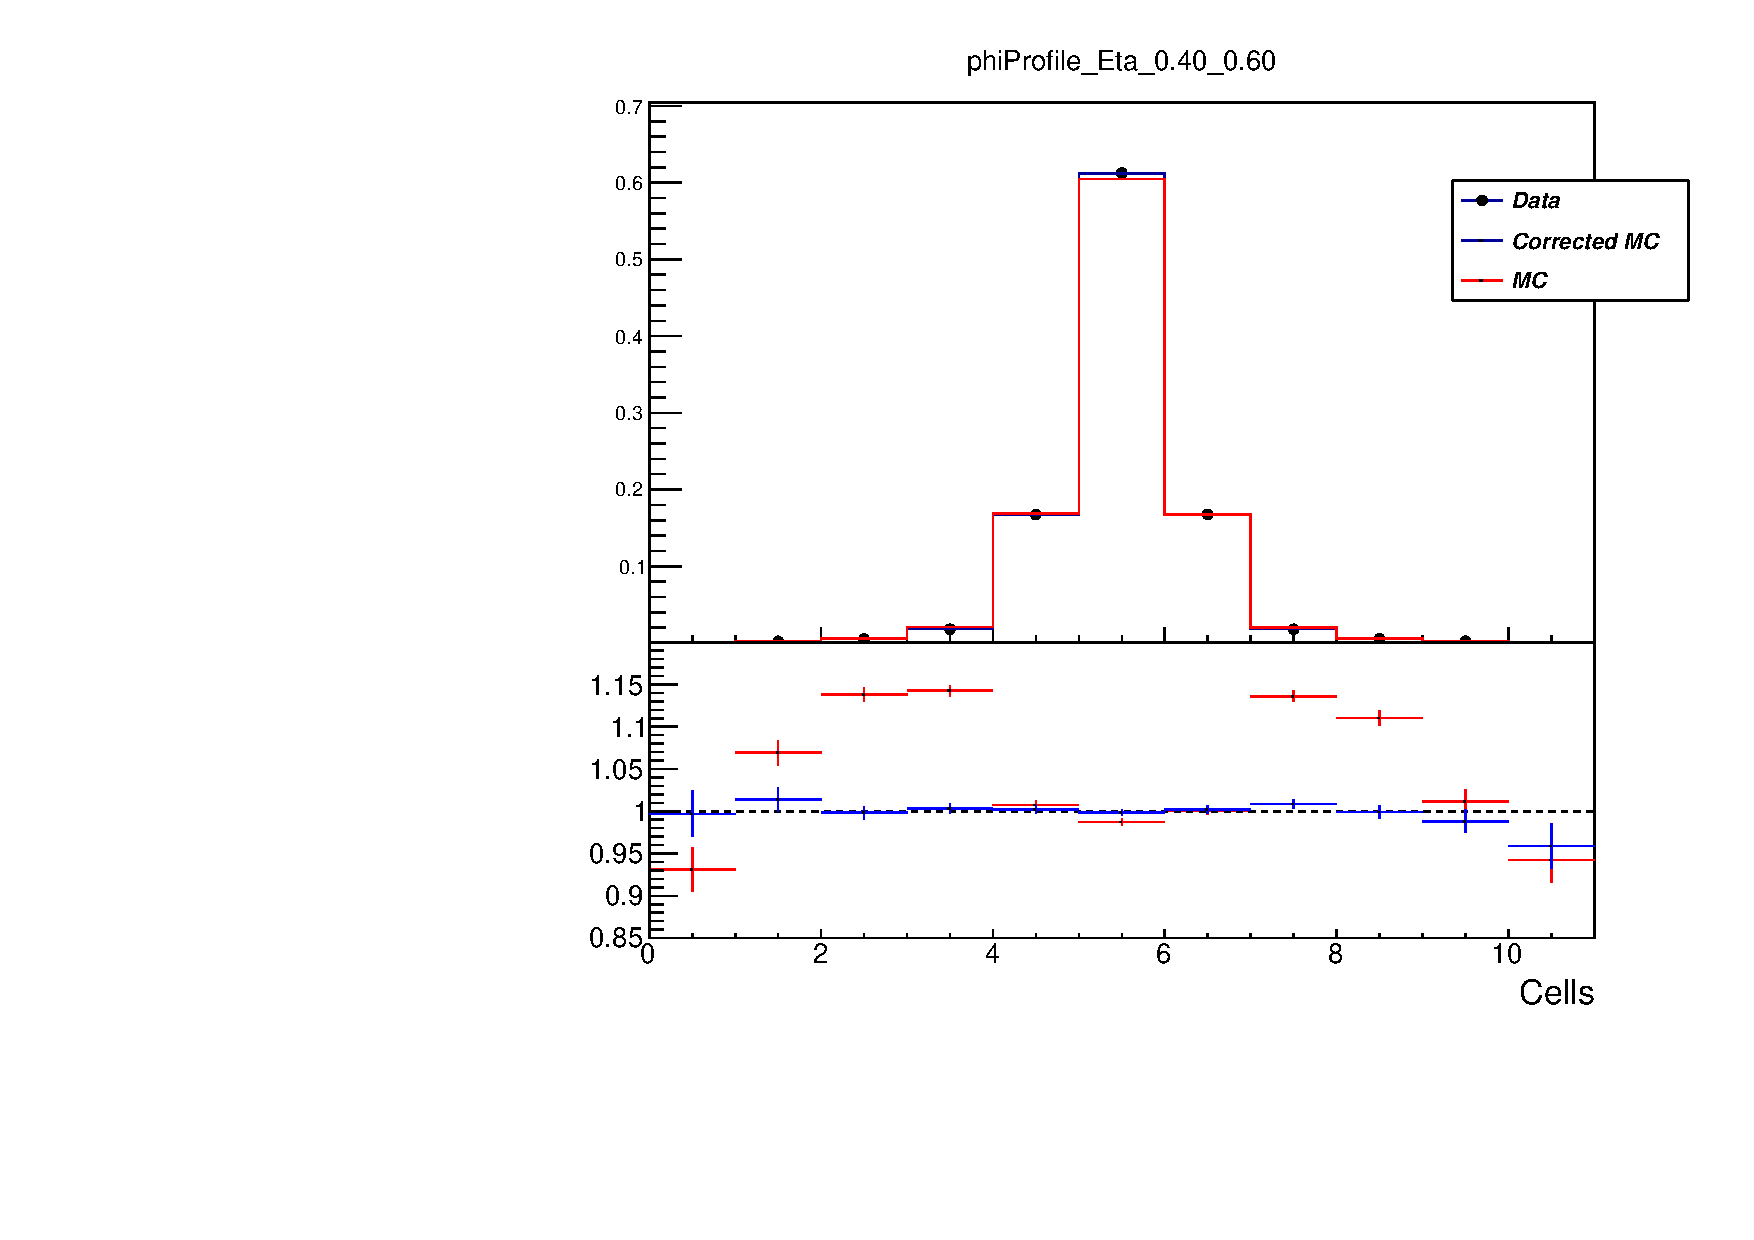
\includegraphics[width=6cm]{phiProfile_Rew_Eta_4_6_Local_Rew_noBS.pdf}\\
\end{columns}
\end{frame}
%------------------------------------------------


%------------------------------------------------
\begin{frame}
\frametitle{<eLeak> vs $\eta$}

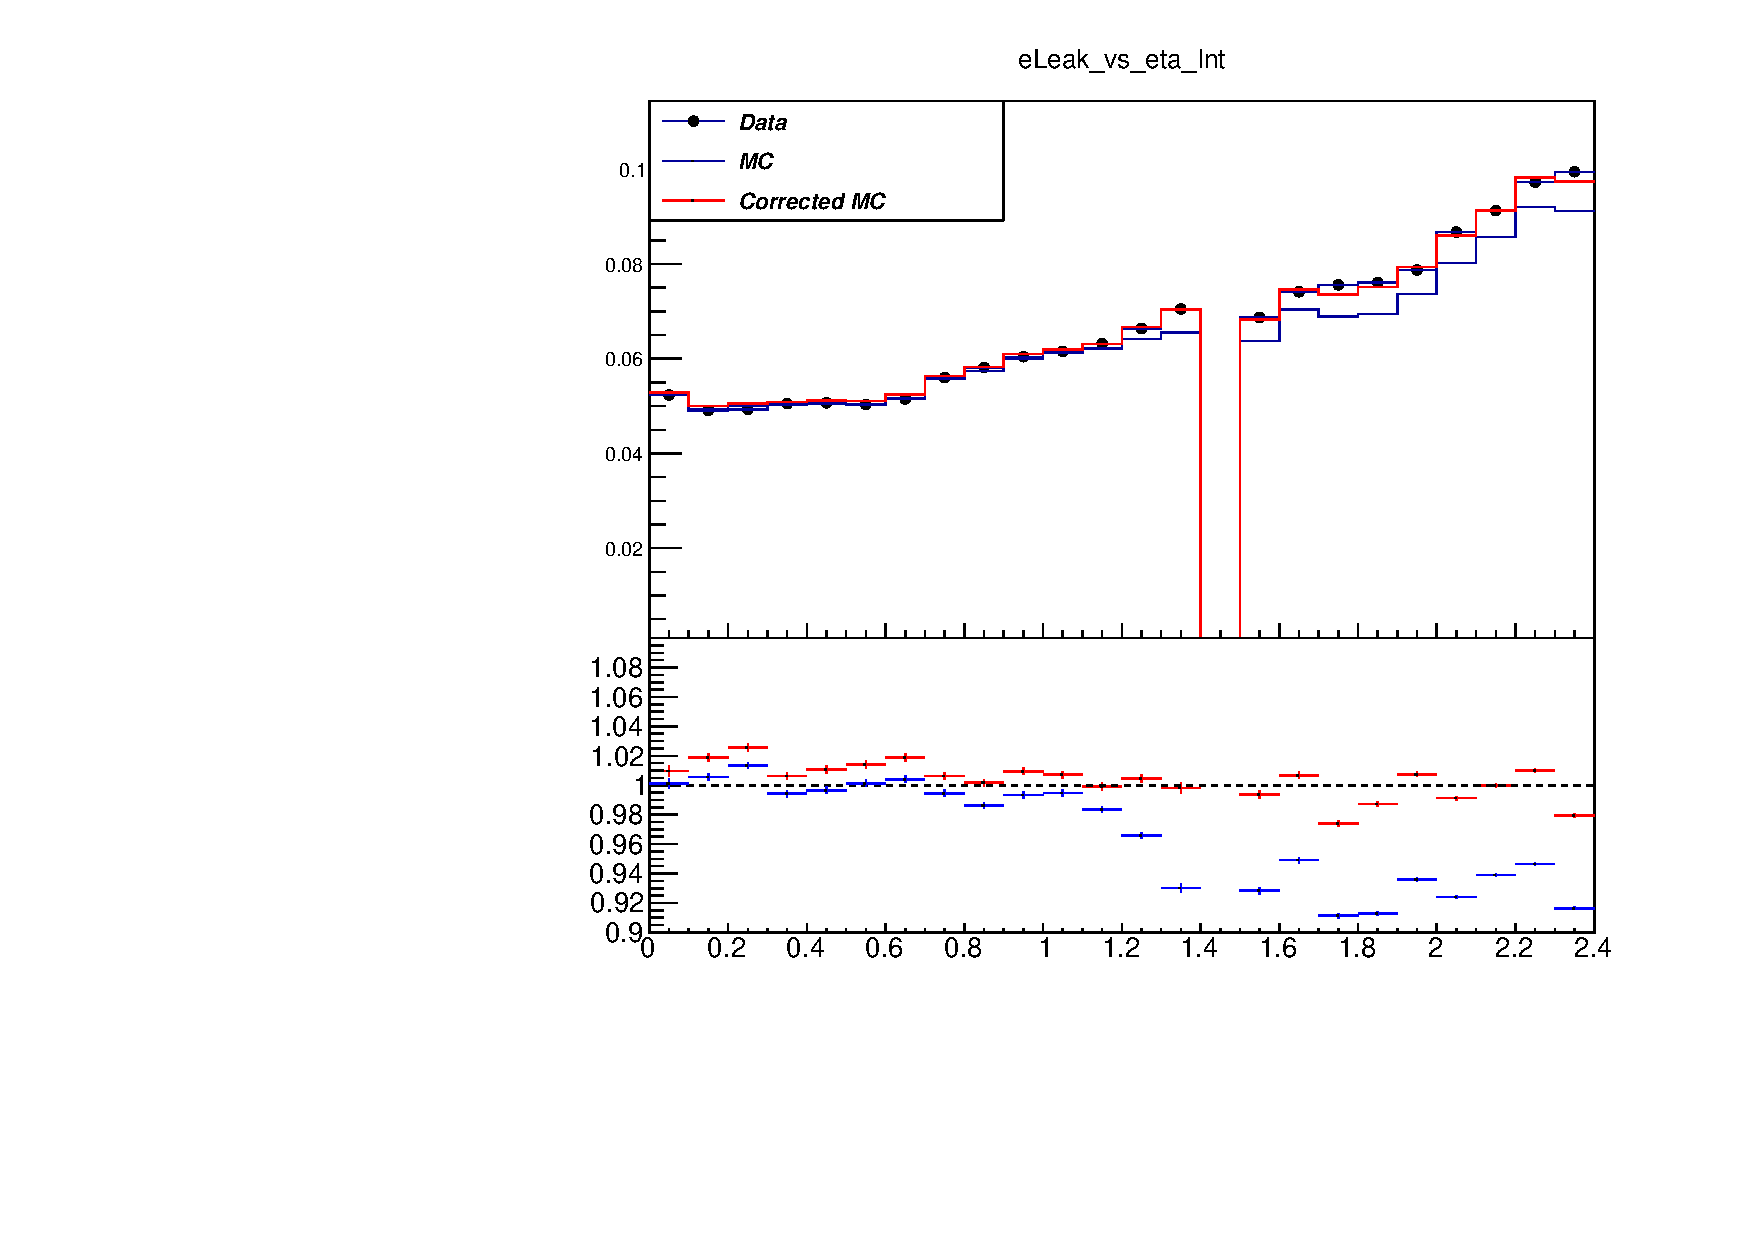
\includegraphics[height=7cm]{eLeak_vs_eta_Int.pdf}
\centering

$eLeak = E_{7x11}/E_{3x7} - 1$
\end{frame}
%------------------------------------------------
%------------------------------------------------
\begin{frame}
\frametitle{Reweighting steps}
\begin{itemize}
\item Local closure test \textcolor{red}{ $\checkmark$}\\
\item Local test for Bremstrahlung subtraction \textcolor{red}{ $\checkmark$}\\
\item Athena closure test - reweighting complete clusters exclusively must reproduce local run with BS subtraction \textcolor{red}{ $\checkmark$}\\
\item Athena run on complete + incomplete clusters\\
\end{itemize}
\end{frame}
%------------------------------------------------
%------------------------------------------------
\begin{frame}
\frametitle{Reweighting incomplete clusters in Athena}
\centering
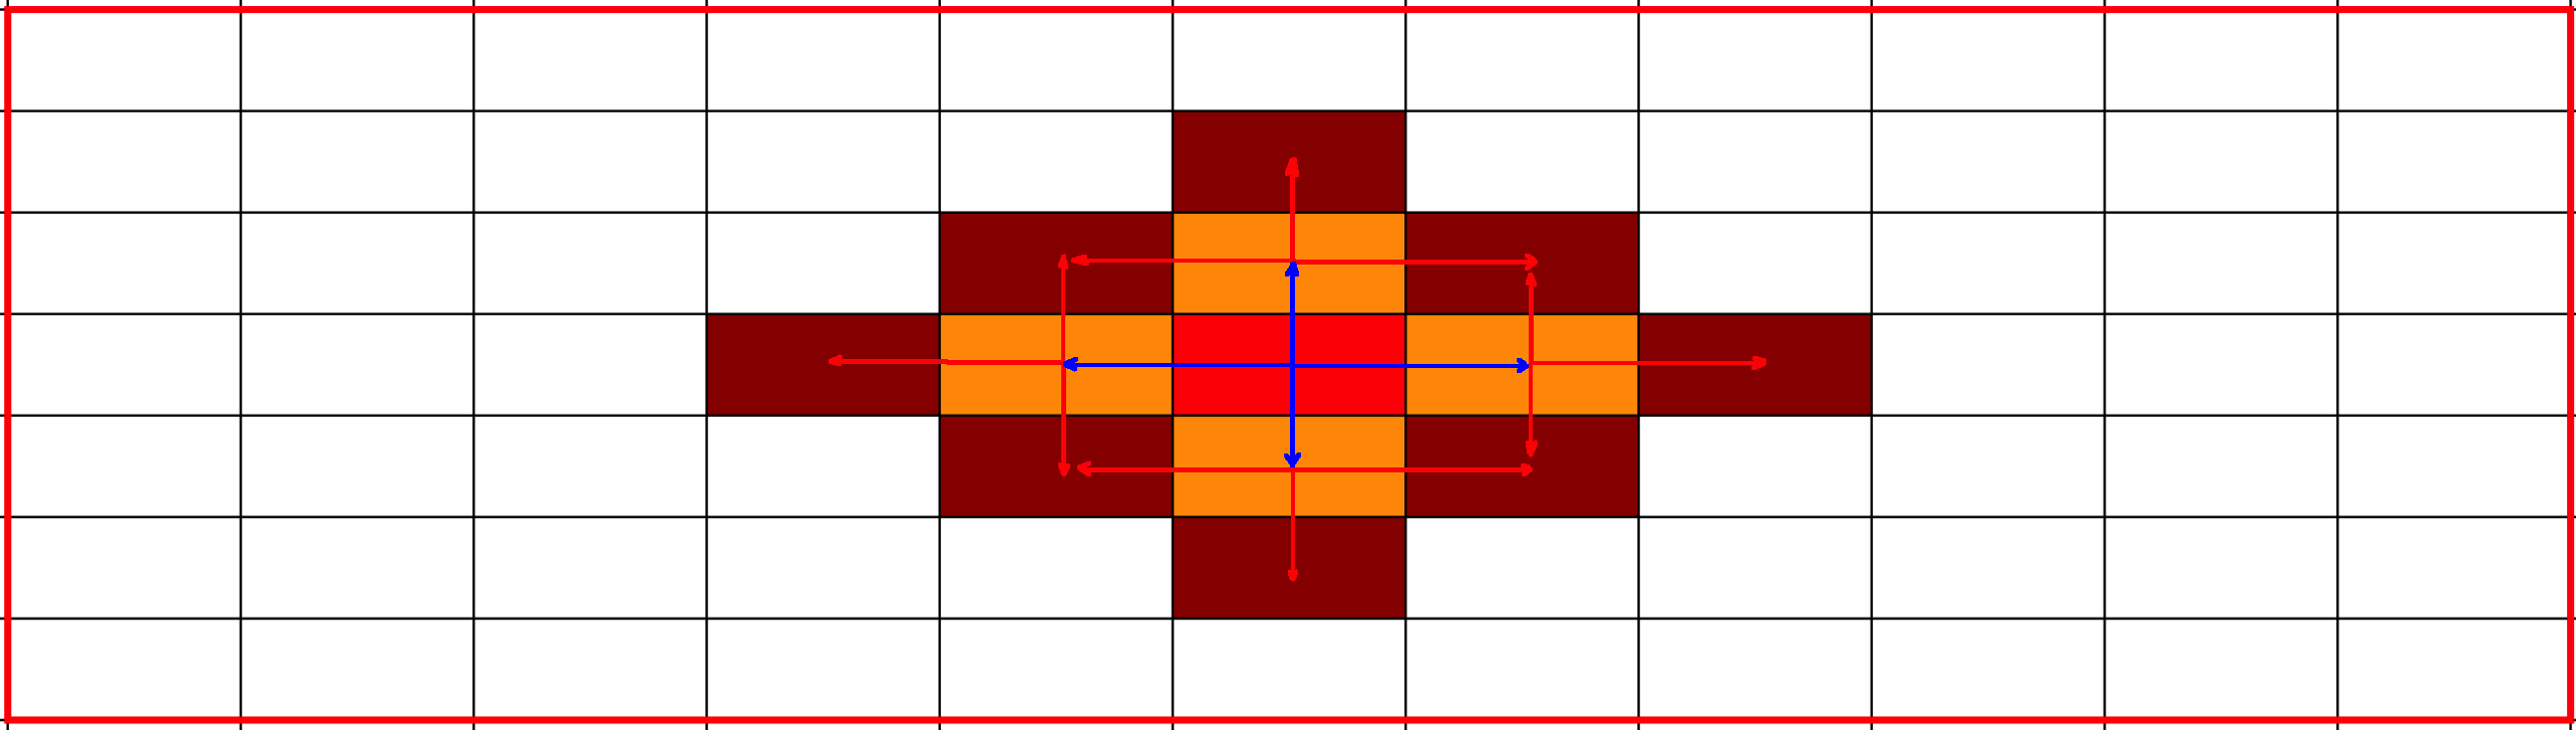
\includegraphics[width=10cm,height=4cm]{cluster_mapping.png}\\
\begin{itemize}
\item CaloIDHelper class CaloCell\_ID "knows" the calorimeter geometry and relative position of every cell through method get\_neighbours(nextInPhi, prevInEta) etc. 
\item A recursive function that gets the IdentifierHash of the seed cell (hottest cell) then goes over the neighbouring cells and so on, creating a cluster map and avoiding crashes.
\item The reweighting coefficients are derived from complete clusters, so some degradation is expected.
\end{itemize}


\end{frame}
%------------------------------------------------


%------------------------------------------------
\begin{frame}
\frametitle{$R_\eta$ with incomplete (left) vs complete clusters (right), $\eta \in (1.8, 2.0)$ }

\begin{columns}[t]
\column{.5\textwidth}
\centering
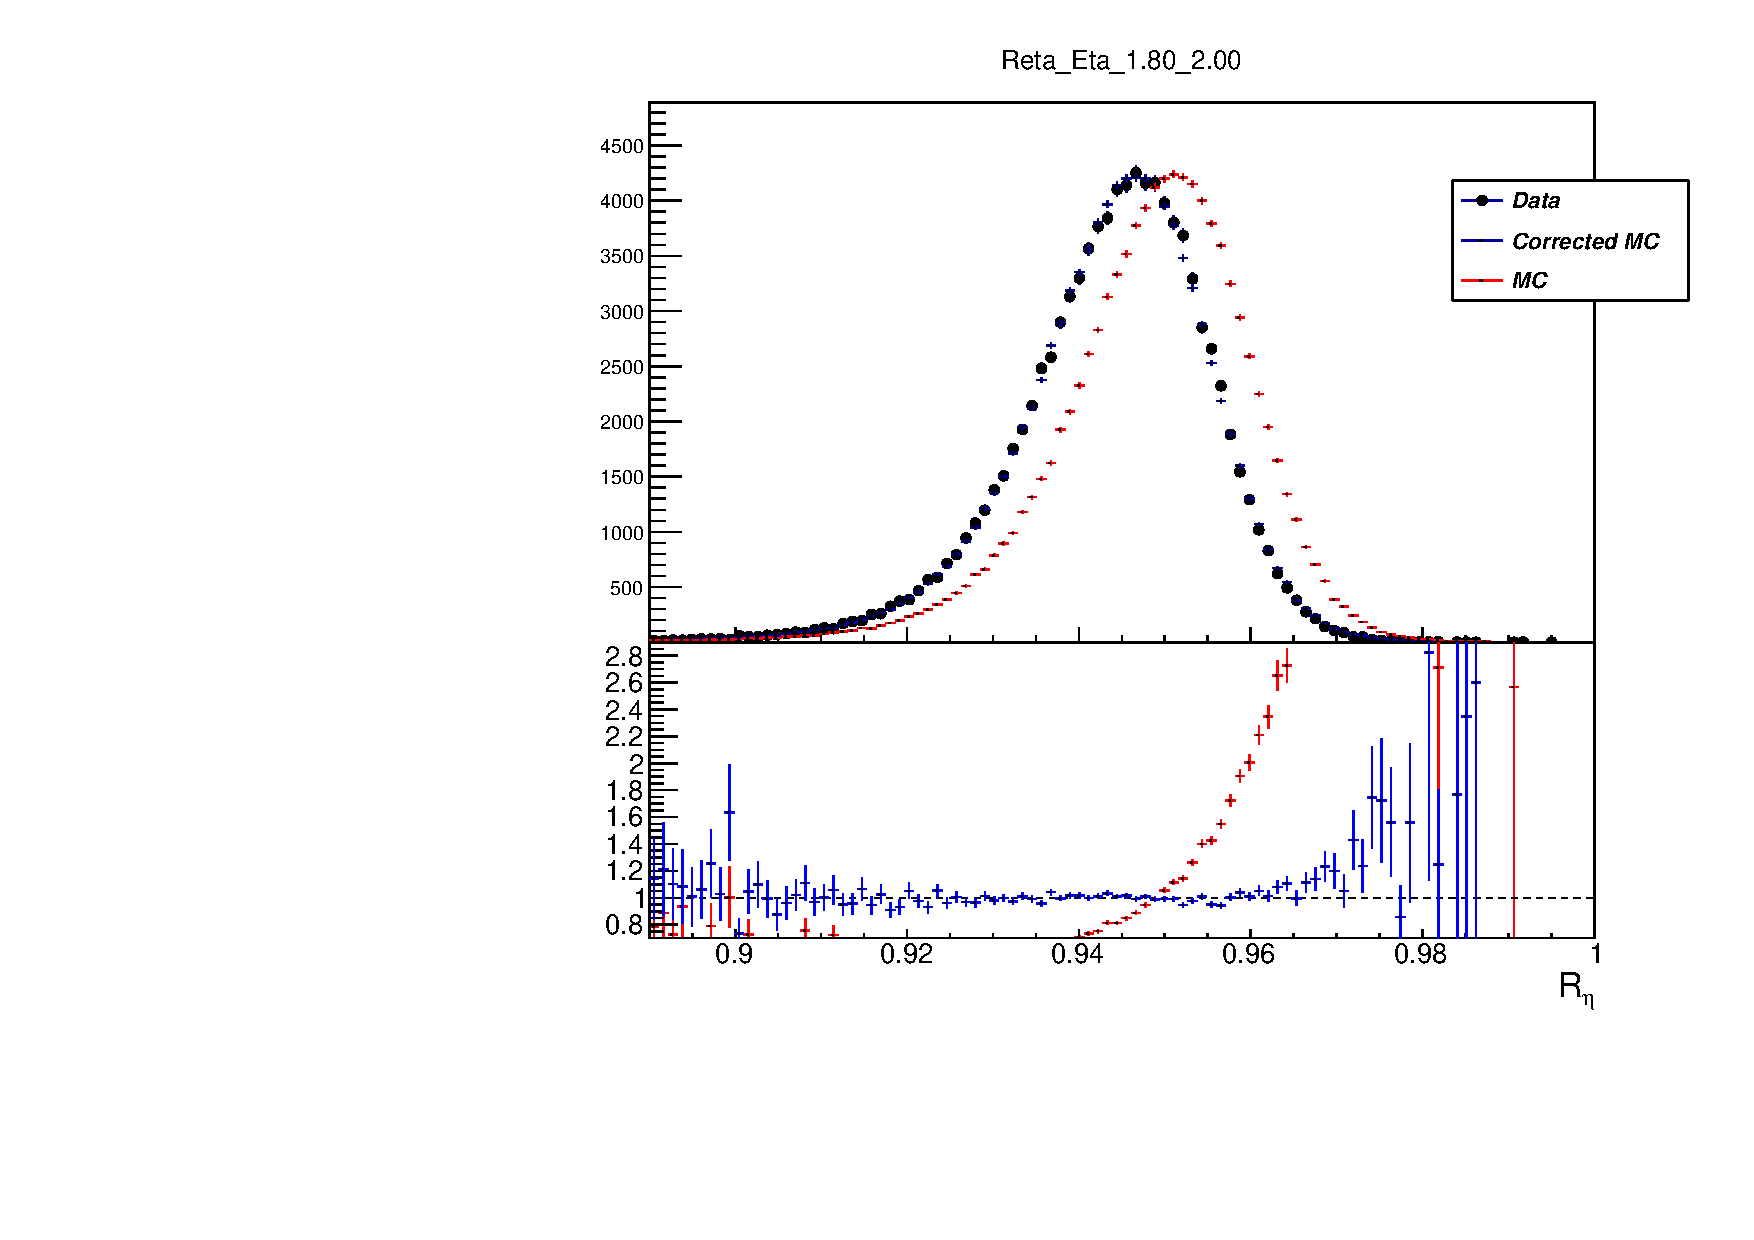
\includegraphics[width=6cm]{Reta_Eta_18_20.pdf}
\column{.5\textwidth}
\centering
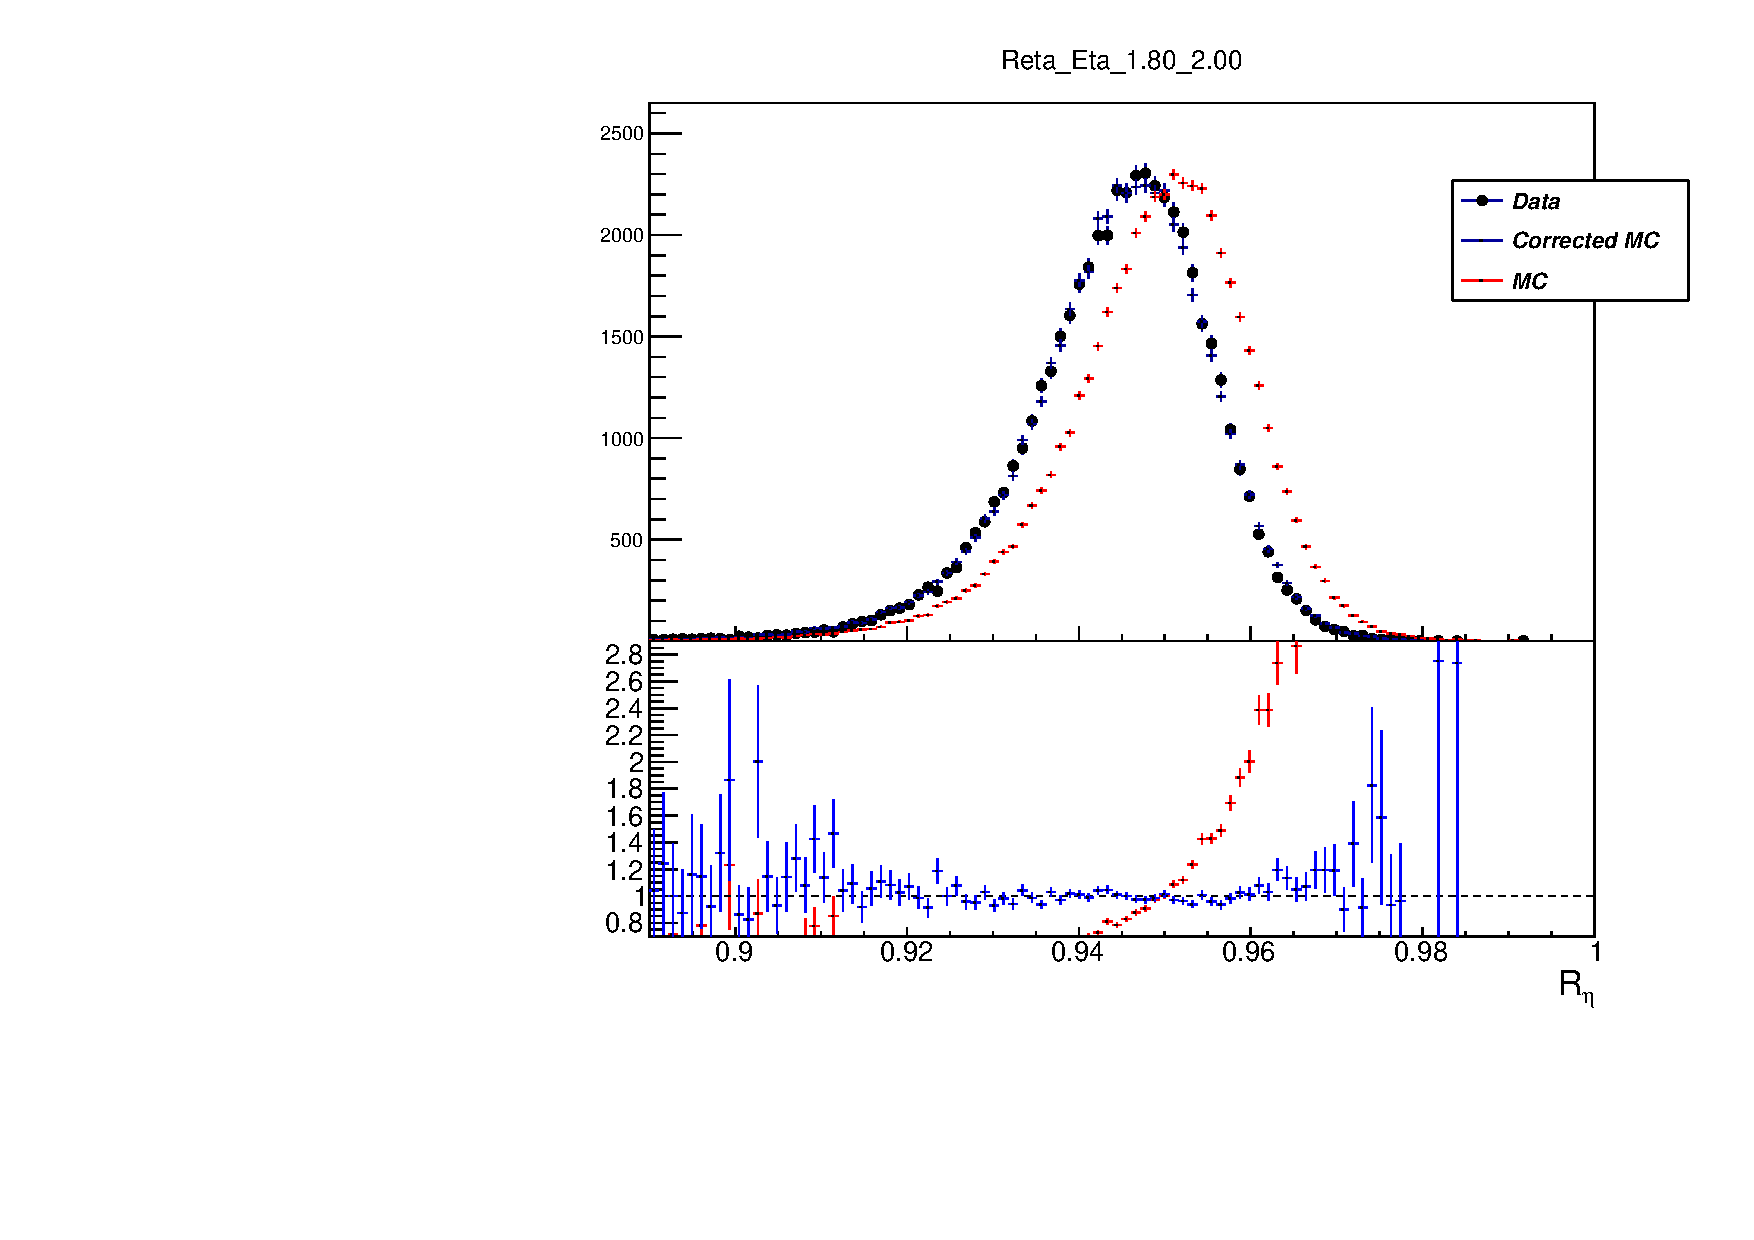
\includegraphics[width=6cm]{Reta_Eta_18_20_Athena.pdf}
\end{columns}
\end{frame}
%------------------------------------------------
%------------------------------------------------
\begin{frame}
\frametitle{$R_\phi$ with incomplete  (left) vs complete clusters (right), $\eta \in (0.4, 0.6)$ }

\begin{columns}[t]
\column{.5\textwidth}
\centering
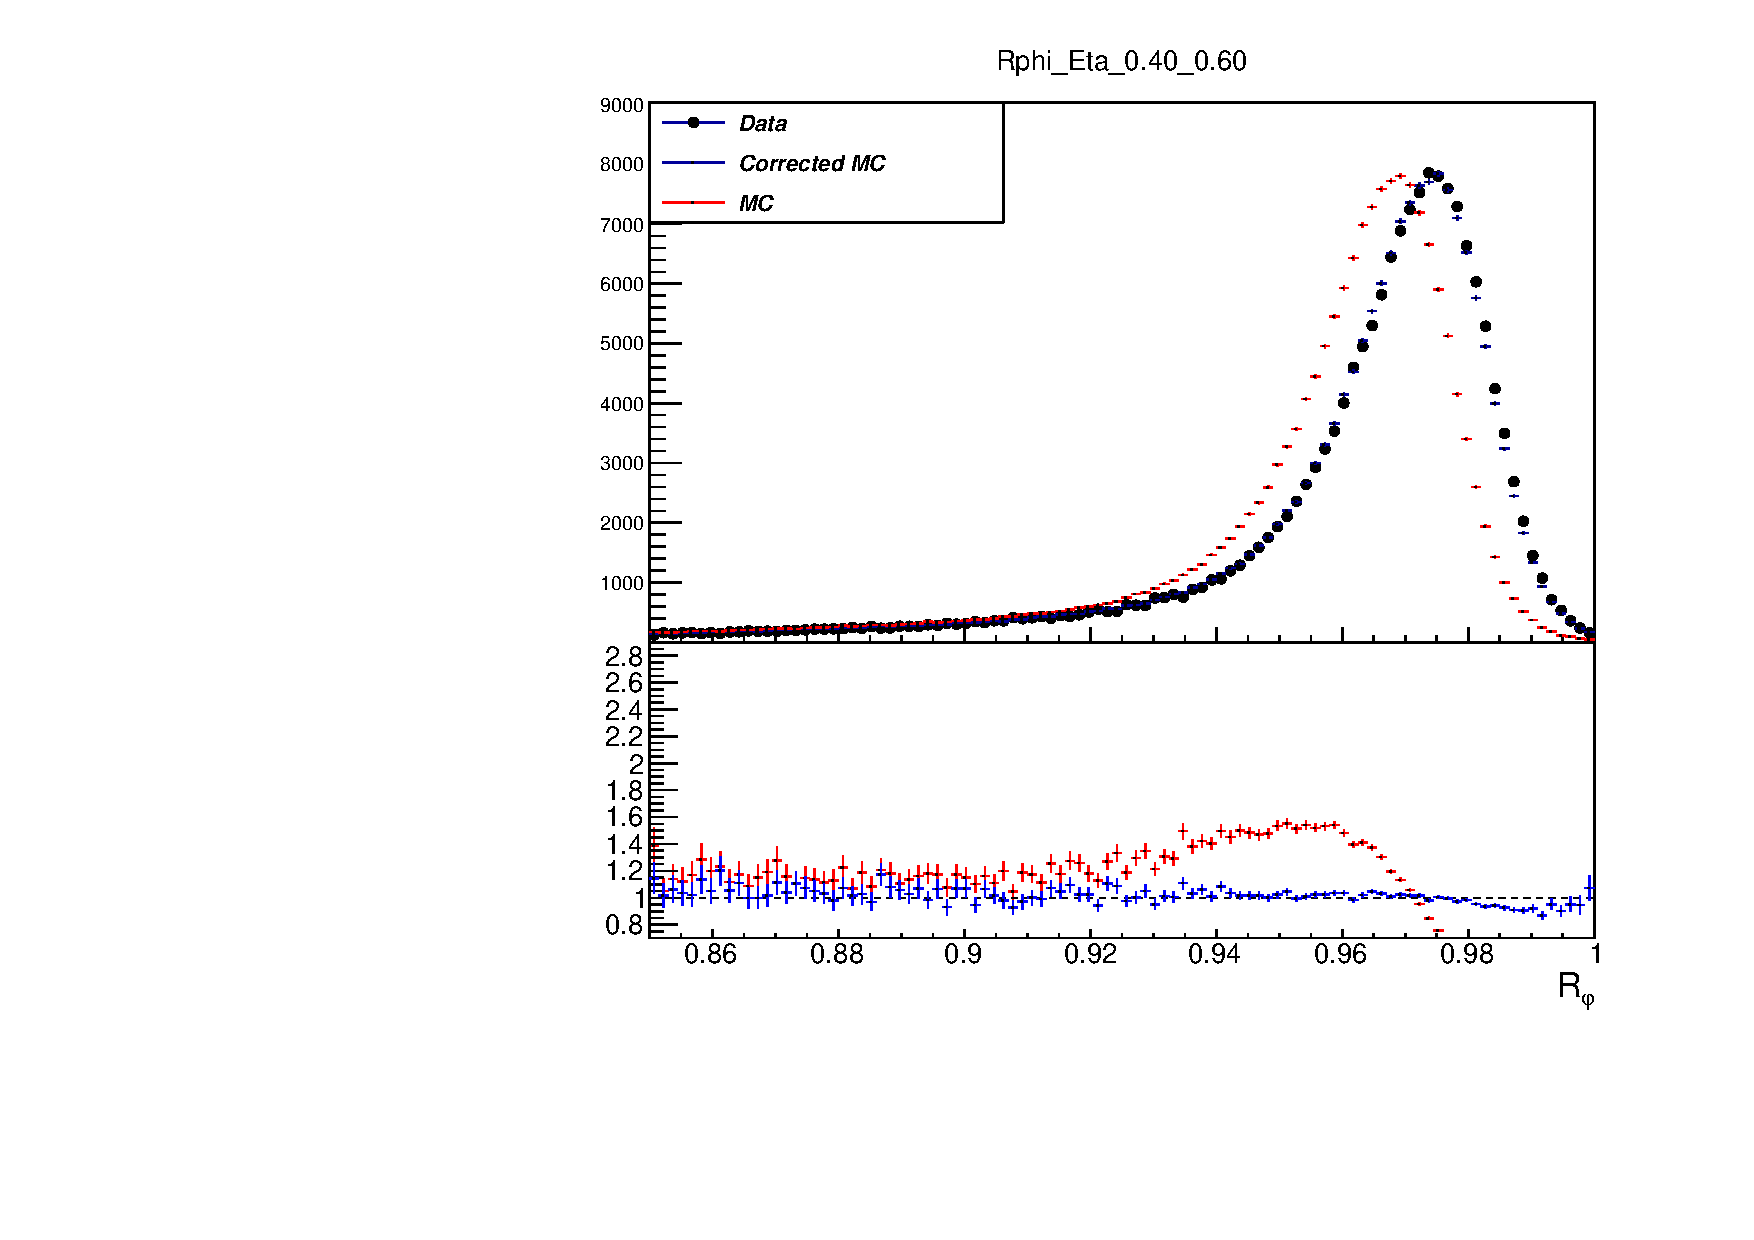
\includegraphics[width=6cm]{Rphi_Eta_4_6.pdf}\\
\column{.5\textwidth}
\centering
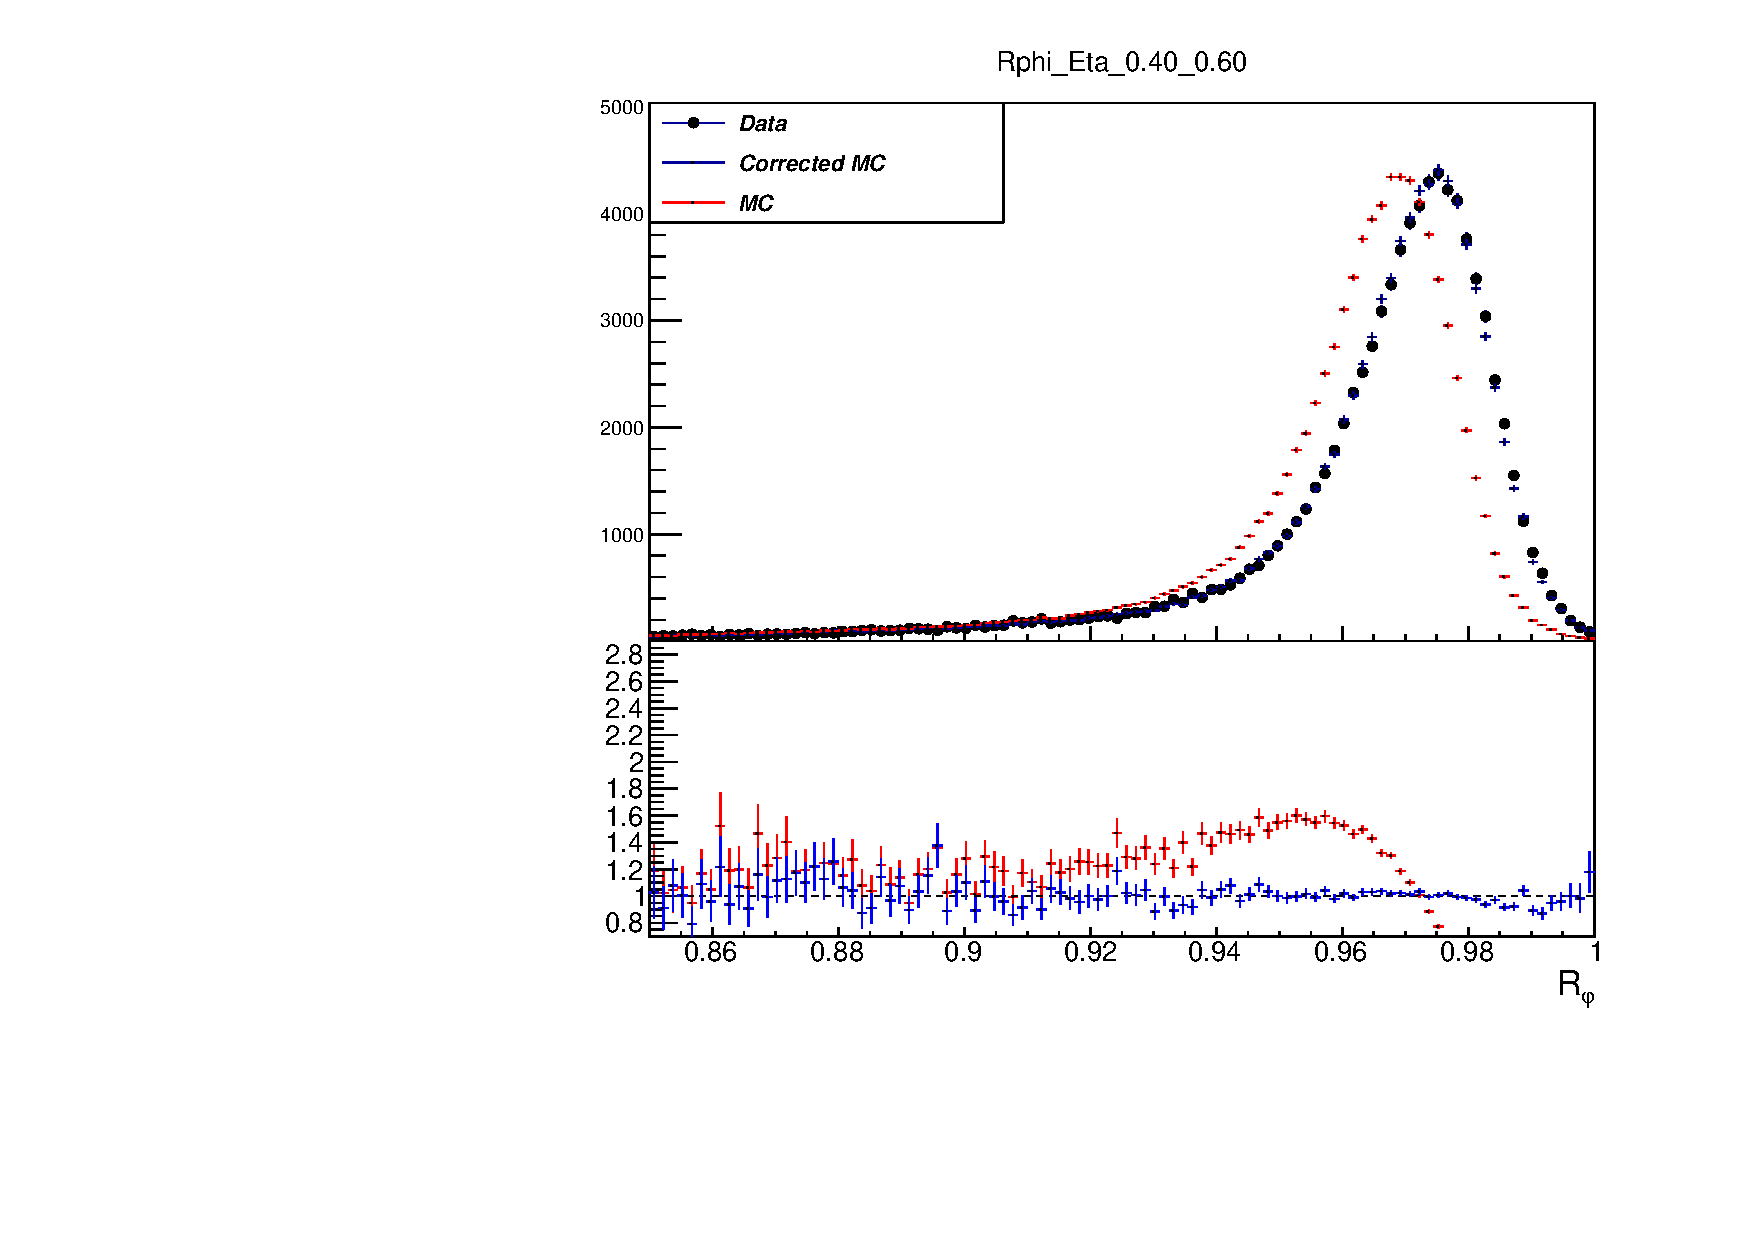
\includegraphics[width=6cm]{Rphi_Eta_4_6_Athena.pdf}\\
\end{columns}
\end{frame}
%------------------------------------------------


%------------------------------------------------
\begin{frame}
\frametitle{$W_{\eta^2}$  with incomplete  (left) vs complete clusters (right), $\eta \in (1.8, 2.0)$ }

\begin{columns}[t]
\column{.5\textwidth}
\centering
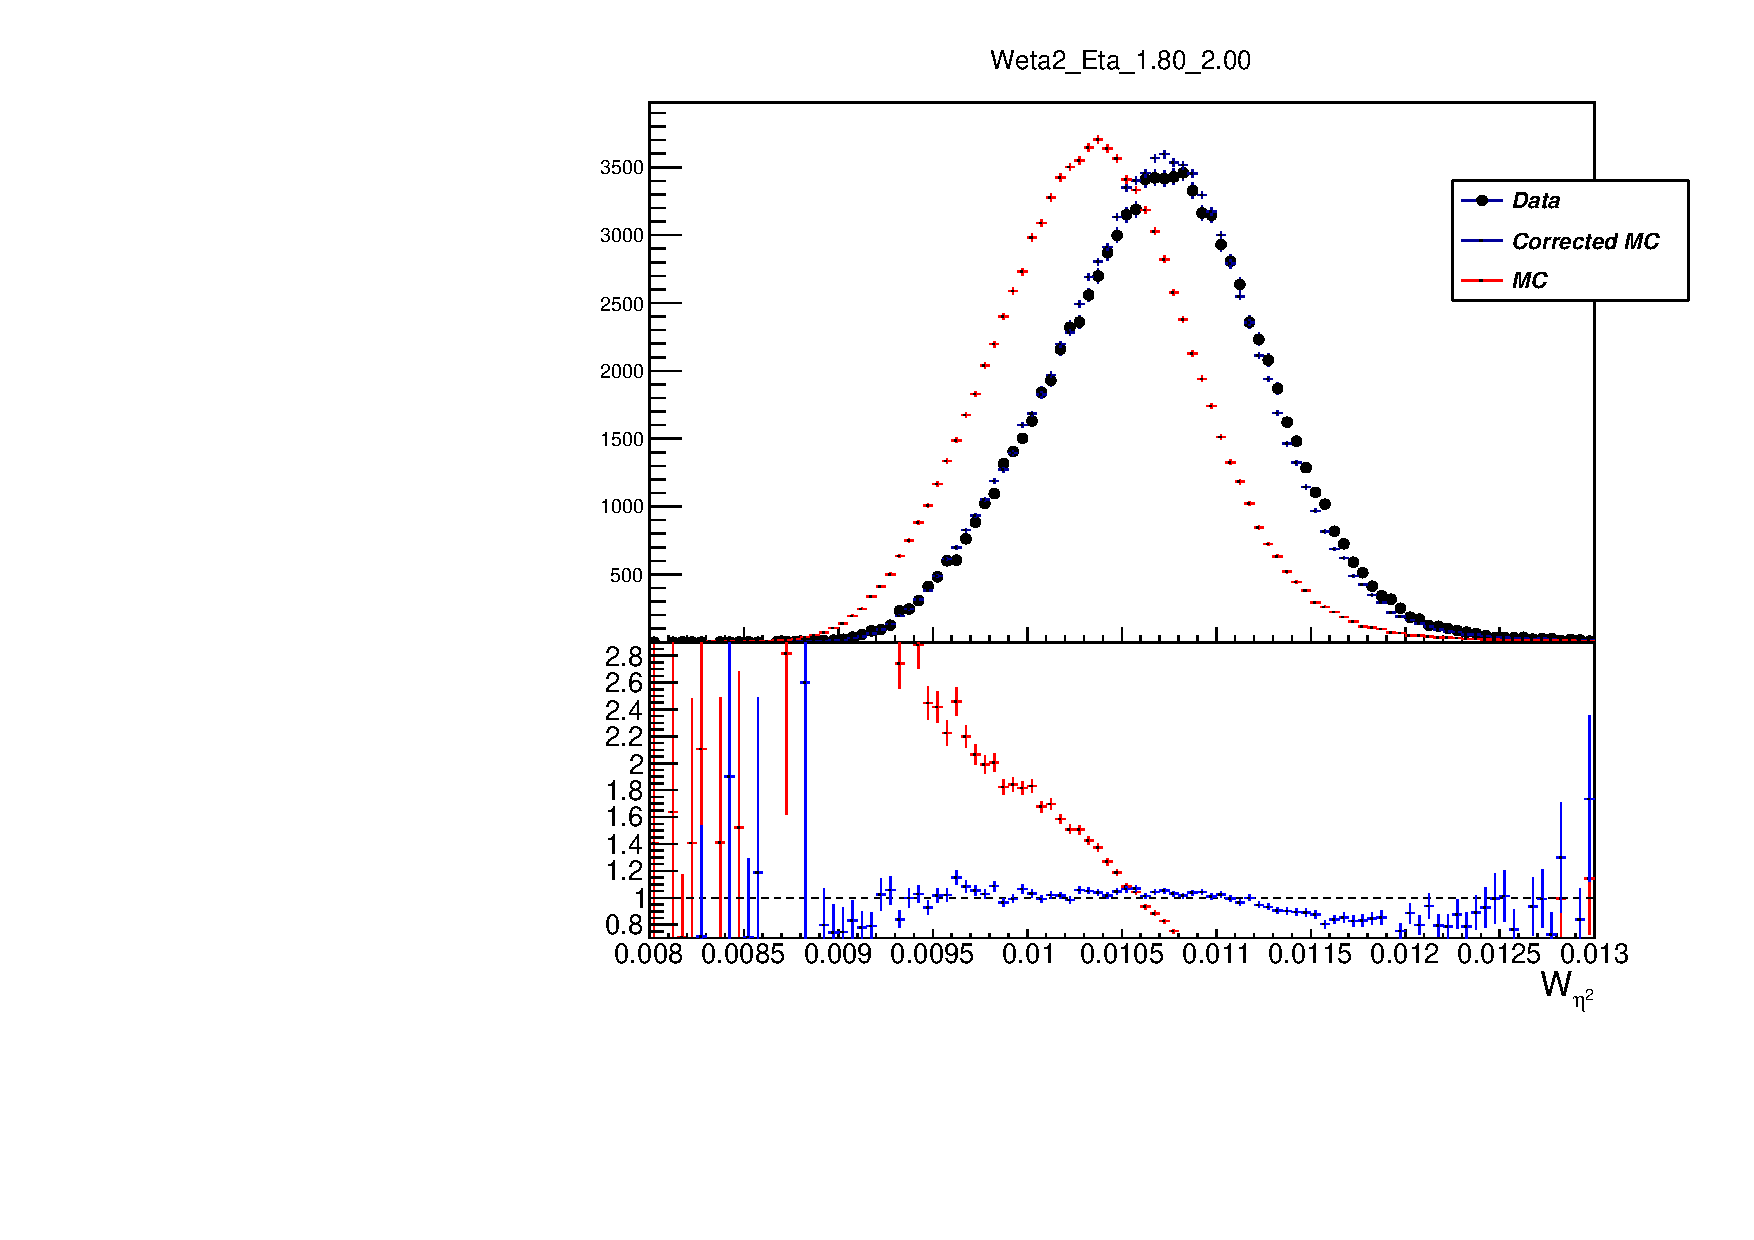
\includegraphics[width=6cm]{Weta2_Eta_18_20.pdf}
\column{.5\textwidth}
\centering
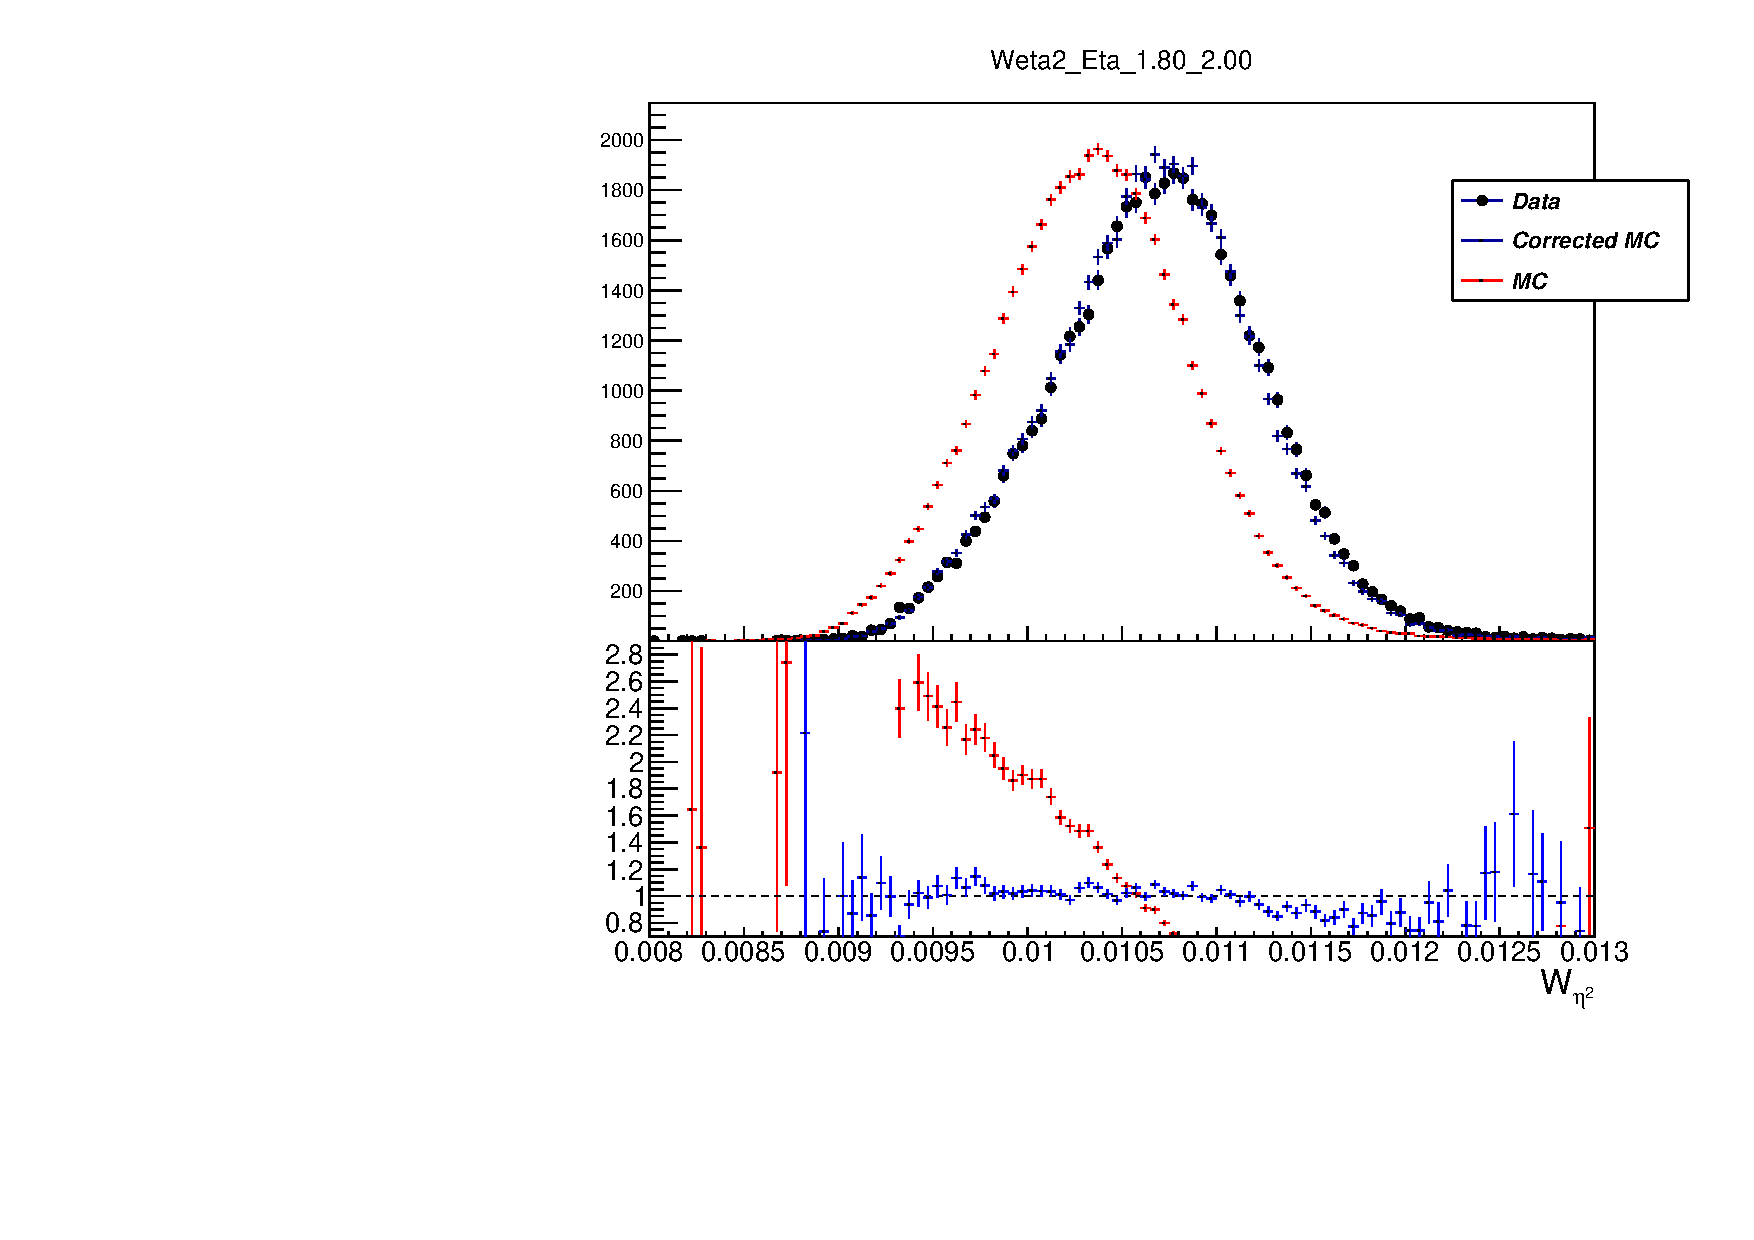
\includegraphics[width=6cm]{Weta2_Eta_18_20_Athena.pdf}
\end{columns}
\end{frame}
%------------------------------------------------

%------------------------------------------------
\begin{frame}
\frametitle{ <$R_\eta$> vs $pT$, incomplete (left) vs complete clusters (right)}

\begin{columns}[t]
\column{.5\textwidth}
\centering
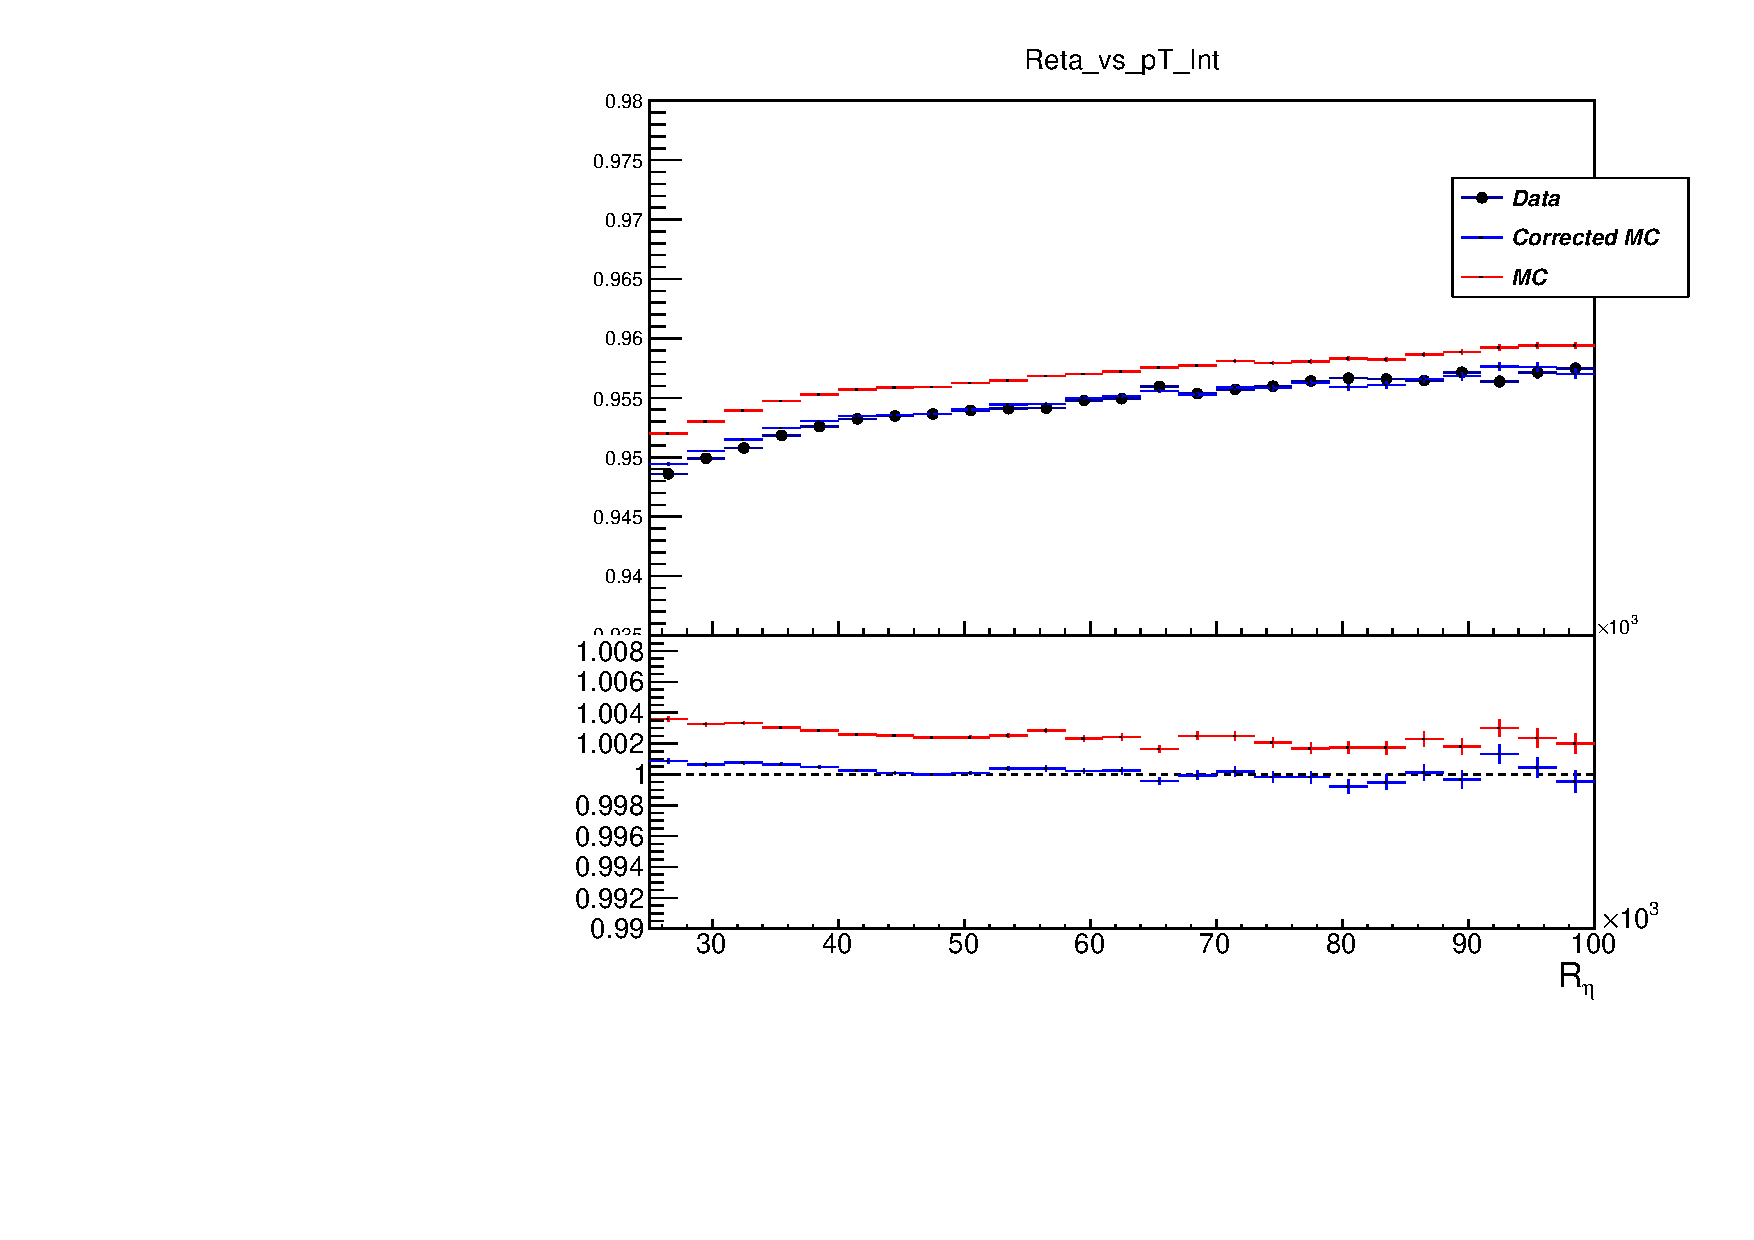
\includegraphics[width=6cm]{Reta_vs_pT_IntSic.pdf}\\
\column{.5\textwidth}
\centering
\includegraphics[width=6cm]{Reta_vs_pT_Int.pdf}\\
\end{columns}
The reweighting appears to be $p_T$-independent and works fine for the inclusive clusters.
\end{frame}
%------------------------------------------------
%------------------------------------------------
\begin{frame}
\frametitle{ <$R_\phi$> vs $pT$, incomplete (left) vs complete clusters (right)}

\begin{columns}[t]
\column{.5\textwidth}
\centering
\includegraphics[width=6cm]{Rphi_vs_pT_IntSic.pdf}
\column{.5\textwidth}
\centering
\includegraphics[width=6cm]{Rphi_vs_pT_Int.pdf}
\end{columns}
\end{frame}
%------------------------------------------------
%------------------------------------------------
\begin{frame}
\frametitle{ <$W_{\eta^2}$> vs $pT$ with incomplete  (left) vs complete clusters (right)}

\begin{columns}[t]
\column{.5\textwidth}
\centering
\includegraphics[width=6cm]{Weta2_vs_pT_IntSic.pdf}\\
\column{.5\textwidth}
\centering
\includegraphics[width=6cm]{Weta2_vs_pT_Int.pdf}\\
\end{columns}
A certain degradation of the reweighting can be seen in <$W_{\eta^2}$>

\end{frame}
%------------------------------------------------

%------------------------------------------------
\begin{frame}
\frametitle{Reweighting steps}
\begin{itemize}
\item Local closure test \textcolor{red}{ $\checkmark$}\\
\item Local test for Bremstrahlung subtraction \textcolor{red}{ $\checkmark$}\\
\item Athena closure test - reweighting complete clusters exclusively must reproduce local run with BS subtraction \textcolor{red}{ $\checkmark$}\\
\item Athena run on complete + incomplete clusters \textcolor{red}{ $\checkmark$}\\


\end{itemize}
\end{frame}
%------------------------------------------------

%------------------------------------------------
\begin{frame}
\frametitle{Efficiency/SF}
\centering

\includegraphics[width=9cm]{MCeffm247tom237.png}\\

\end{frame}

%------------------------------------------------

%------------------------------------------------
\begin{frame}
\frametitle{Low $\mu$ run, $\eta$ profile, $\eta \in (2.0,2.4)$}

\begin{columns}[t]

\column{.5\textwidth}
\centering
\normalsize{Dedicated low-mu reweighting}
\includegraphics[width=6cm]{etaProfile_Rew_Eta_20_24_lowmu_13TeV_LocalWB.pdf}
\column{.5\textwidth}
\centering
\normalsize{Using high-mu reweighting}
\includegraphics[width=6cm]{etaProfile_Eta_20_24_lowmu_13TeV_AthenaWB.pdf}
\end{columns}
\end{frame}
%------------------------------------------------
%------------------------------------------------
\begin{frame}
\frametitle{Low $\mu$ run, $\phi$ profile, $\eta \in (0,0.6)$}

\begin{columns}[t]

\column{.5\textwidth}
\centering
\normalsize{Dedicated low-mu reweighting}
\includegraphics[width=6cm]{phiProfile_Rew_Eta_0_6_lowmu_13TeV_LocalWB.pdf}\\
\column{.5\textwidth}
\centering
\normalsize{High-mu reweighting}
\includegraphics[width=6cm]{phiProfile_Eta_0_6_lowmu_13TeV_AthenaWB.pdf}\\
\end{columns}
\end{frame}
%------------------------------------------------

%------------------------------------------------
\begin{frame}
\frametitle{Low $\mu$ run, $R_{\eta}$ profile, $\eta \in (2.0,2.4)$}

\begin{columns}[t]

\column{.5\textwidth}
\centering
\normalsize{Dedicated low-mu reweighting}
\includegraphics[width=6cm]{Reta_Rew_Eta_20_24_lowmu_13TeV_LocalWB.pdf}
\column{.5\textwidth}
\centering
\normalsize{Using high-mu reweighting}
\includegraphics[width=6cm]{Reta_Eta_20_24_lowmu_13TeV_AthenaWB.pdf}
\end{columns}
\end{frame}
%------------------------------------------------
%------------------------------------------------
\begin{frame}
\frametitle{Low $\mu$ run, $R_{\phi}$, $\eta \in (0,0.6)$}

\begin{columns}[t]

\column{.5\textwidth}
\centering
\normalsize{Dedicated low-mu reweighting}
\includegraphics[width=6cm]{Rphi_Rew_Eta_0_6_lowmu_13TeV_LocalWB.pdf}\\
\column{.5\textwidth}
\centering
\normalsize{High-mu reweighting}
\includegraphics[width=6cm]{Rphi_Eta_0_6_lowmu_13TeV_AthenaWB.pdf}\\
\end{columns}
\end{frame}
%------------------------------------------------




%------------------------------------------------
\begin{frame}
\frametitle{Non-converted photons $R_\eta$, $\eta \in (0, 1.37)$ , $(1.52, 2.37)$}

\begin{columns}[t]
\column{.5\textwidth}
\centering
\includegraphics[width=6cm]{Reta_NConv_0_137.pdf}\\
\column{.5\textwidth}
\centering
\includegraphics[width=6cm]{Reta_NConv_152_237.pdf}\\
\end{columns}
\end{frame}
%------------------------------------------------
%------------------------------------------------
\begin{frame}
\frametitle{Non-converted photons $R_\phi$, $\eta \in (0, 1.37)$ , $(1.52, 2.37)$}

\begin{columns}[t]
\column{.5\textwidth}
\centering
\includegraphics[width=6cm]{Rphi_NConv_0_137.pdf}\\
\column{.5\textwidth}
\centering
\includegraphics[width=6cm]{Rphi_NConv_152_237.pdf}\\
\end{columns}
Thanks Mohamed for the plots.
\end{frame}
%------------------------------------------------
%------------------------------------------------
\begin{frame}
\frametitle{Conclusions}

\begin{itemize}
\item The developed method was aimed to make the ID efficiency in MC as close as possible to the data. It is shown to have a visible positive effect, notably in the endcap region.
\item The reweighting is pT-independent.
\item It seems that high-mu reweighting coefficients work reasonably well for the low-mu samples - gives an idea that the dependence on pile-up is not very strong.
\item To be presented for approval as a part of an official Athena release. 
\item Technical note is in development and to be presented soon. 
\item A study on photon shower shapes reweighting is now performed by Mohamed Belfkir.

\end{itemize}

\end{frame}

%------------------------------------------------
\begin{frame}
\frametitle{BACKUP}

\begin{itemize}
\item BACKUP SLIDES
\end{itemize}

\end{frame}

%------------------------------------------------
%------------------------------------------------

\begin{frame}
\begin{columns}[t]
\frametitle{Efficiencies and SF - medium and tight}
\column{.5\textwidth}
\centering
\includegraphics[width=6cm,height=4cm]{Efficiencies_Eta_EB_Medium.png}\\
\includegraphics[width=6cm,height=4cm]{Efficiencies_Eta_EB_Tight.png}
\column{.5\textwidth}
\centering
\includegraphics[width=6cm,height=4cm]{Efficiencies_pT_EB_Medium.png}\\
\includegraphics[width=6cm,height=4cm]{Efficiencies_pT_EB_Tight.png}
\end{columns}
\end{frame}
%------------------------------------------------
%------------------------------------------------
\begin{frame}
\frametitle{$R_\eta$ with incomplete (left) vs complete clusters (right), $\eta \in (0.4, 0.6)$ }

\begin{columns}[t]
\column{.5\textwidth}
\centering
\includegraphics[width=6cm]{Reta_Eta_4_6.pdf}\\
\column{.5\textwidth}
\centering
\includegraphics[width=6cm]{Reta_Eta_4_6_Athena.pdf}\\
\end{columns}
\end{frame}
%------------------------------------------------
%------------------------------------------------
\begin{frame}
\frametitle{Reweighted Bremsstrahlung-free $R_\eta$, $\eta \in (0.4, 0.6)$ and $(1.8, 2.0)$}

\begin{columns}[t]
\column{.5\textwidth}
\centering
\includegraphics[width=6cm]{Reta_Rew_Eta_18_20_Local_Rew_noBS.pdf}\\

\includegraphics[width=6cm]{Reta_Rew_Eta_4_6_Local_Rew_noBS.pdf}\\
\column{.5\textwidth}
\centering
\end{columns}
\end{frame}
%------------------------------------------------
%------------------------------------------------
\begin{frame}
\frametitle{Reweighted Bremsstrahlung-free $R_\phi$, $\eta \in (0.4, 0.6)$ and $(1.8, 2.0)$}

\begin{columns}[t]
\column{.5\textwidth}
\centering
\includegraphics[width=6cm]{Rphi_Rew_Eta_4_6_Local_Rew_noBS.pdf}\\
\column{.5\textwidth}
\centering
\includegraphics[width=6cm]{Rphi_Rew_Eta_18_20_Local_Rew_noBS.pdf}
\end{columns}
\end{frame}
%------------------------------------------------
%------------------------------------------------

\begin{frame}
\frametitle{Event selection}

\begin{itemize}
\item Z->ee process considered
\item event was required to have two electrons one of which has $p_T>25GeV$
\item  gradient isolation
\item  Tag and probe, no ID 
\item  Z invariant mass window 80 - 120 GeV 
\item  electron triggers: HLT\_e26\_lhtight\_nod0\_ivarloose, HLT\_e60\_lhmedium\_nod0, HLT\_e140\_lhloose\_nod0,HLT\_e300\_etcut
\item no pile-up reweighting
\end{itemize}



\end{frame}
%------------------------------------------------
%------------------------------------------------
\begin{frame}
\frametitle{$R_\phi$ with incomplete  (left) vs complete clusters (right), $\eta \in (1.8, 2.0)$ }

\begin{columns}[t]
\column{.5\textwidth}
\centering
\includegraphics[width=6cm]{Rphi_Eta_18_20.pdf}
\column{.5\textwidth}
\centering
\includegraphics[width=6cm]{Rphi_Eta_18_20_Athena.pdf}
\end{columns}
\end{frame}
%------------------------------------------------
%------------------------------------------------
\begin{frame}
\frametitle{Eta profile - no charge asymmetry, Data and MC}

\begin{columns}[t]
\column{.5\textwidth}
\centering
\includegraphics[width=6cm,height=4cm]{etaProfileDataMC_Eta_4_6.pdf}\\
\includegraphics[width=6cm,height=4cm]{etaProfileDataMC_Eta_18_20.pdf}
\column{.5\textwidth}
\centering
\includegraphics[width=6cm,height=4cm]{etaProfileDataMC_Eta_10_12.pdf}\\
\includegraphics[width=6cm,height=4cm]{etaProfileDataMC_Eta_20_22.pdf}
\end{columns}
\end{frame}
%------------------------------------------------
%------------------------------------------------
%------------------------------------------------
\begin{frame}
\frametitle{Second layer energy profile}

\centering
\includegraphics[width=12cm,height=8cm]{Energy_Profile_15.png}\\
\end{frame}
%------------------------------------------------
%------------------------------------------------
\begin{frame}
\frametitle{$W_{\eta^2}$  with incomplete  (left) vs complete clusters (right), $\eta \in (0.4, 0.6)$ }

\begin{columns}[t]
\column{.5\textwidth}
\centering
\includegraphics[width=6cm]{Weta2_Eta_4_6.pdf}\\
\column{.5\textwidth}
\centering
\includegraphics[width=6cm]{Weta2_Eta_4_6_Athena.pdf}\\
\end{columns}
\end{frame}
%------------------------------------------------

\begin{frame}
\frametitle{Excerpt from the previous study - $R_{\eta}$ and $W_{\eta^2}$ }

\begin{figure}
\centering
\includegraphics[width=11cm]{Screen_Shot.png}\\
\end{figure}

\end{frame}
%------------------------------------------------
\begin{frame}
\frametitle{Wtots1}

\begin{columns}[t]
\column{.5\textwidth}
\centering
\includegraphics[width=6cm,height=4cm]{wtots1_Eta_4_6.pdf}\\
\includegraphics[width=6cm,height=4cm]{wtots1_Eta_8_10.pdf}
\column{.5\textwidth}
\centering
\includegraphics[width=6cm,height=4cm]{wtots1_Eta_16_18.pdf}\\
\includegraphics[width=6cm,height=4cm]{wtots1_Eta_20_22.pdf}
\end{columns}
\end{frame}

%------------------------------------------------

\begin{frame}
\frametitle{Athena derivation reweighting (right) vs local test (left), $\eta$ profile, $\eta \in (1.8, 2.0)$, complete clusters only}

\begin{columns}[t]

\column{.5\textwidth}
\centering
\includegraphics[width=6cm]{etaProfile_Eta_18_20_Athena.pdf}\\
\column{.5\textwidth}
\centering
\includegraphics[width=6cm]{etaProfile_Rew_Eta_18_20_Local_Rew_noBS.pdf}\\
\end{columns}
\end{frame}
%------------------------------------------------
%------------------------------------------------

\begin{frame}
\frametitle{Athena derivation reweighting (right) vs local test (left), $\phi$ profile, $\eta \in (1.8, 2.0)$, complete clusters only}

\begin{columns}[t]

\column{.5\textwidth}
\centering
\includegraphics[width=6cm]{phiProfile_Eta_18_20_Athena.pdf}\\
\column{.5\textwidth}
\centering
\includegraphics[width=6cm]{phiProfile_Rew_Eta_18_20_Local_Rew_noBS.pdf}\\
\end{columns}
\end{frame}
%------------------------------------------------
%------------------------------------------------
\begin{frame}
\frametitle{Low $\mu$ run, $\eta$ profile, $\eta \in (0,0.6)$}

\begin{columns}[t]

\column{.5\textwidth}
\centering
\normalsize{Special low-mu reweighting}
\includegraphics[width=6cm]{etaProfile_Rew_Eta_0_6_lowmu_13TeV_LocalWB.pdf}\\
\column{.5\textwidth}
\centering
\normalsize{High-mu reweighting}
\includegraphics[width=6cm]{etaProfile_Eta_0_6_lowmu_13TeV_AthenaWB.pdf}\\
\end{columns}
\end{frame}
%------------------------------------------------
%------------------------------------------------
\begin{frame}
\frametitle{Low $\mu$ run, $\phi$ profile, $\eta \in (2.0,2.4)$}

\begin{columns}[t]

\column{.5\textwidth}
\centering
\big{Dedicated low-mu reweighting}
\includegraphics[width=6cm]{phiProfile_Rew_Eta_20_24_lowmu_13TeV_LocalWB.pdf}
\column{.5\textwidth}
\centering
\big{Using high-mu reweighting}
\includegraphics[width=6cm]{phiProfile_Eta_20_24_lowmu_13TeV_AthenaWB.pdf}
\end{columns}
\end{frame}
%------------------------------------------------
%------------------------------------------------
\begin{frame}
\frametitle{Low $\mu$ run, $R_{\eta}$, $\eta \in (0,0.6)$}

\begin{columns}[t]

\column{.5\textwidth}
\centering
\normalsize{Special low-mu reweighting}
\includegraphics[width=6cm]{Reta_Rew_Eta_0_6_lowmu_13TeV_LocalWB.pdf}\\
\column{.5\textwidth}
\centering
\normalsize{High-mu reweighting}
\includegraphics[width=6cm]{Reta_Eta_0_6_lowmu_13TeV_AthenaWB.pdf}\\
\end{columns}
\end{frame}
%------------------------------------------------
%------------------------------------------------
\begin{frame}
\frametitle{Low $\mu$ run, $R_{\phi}$ profile, $\eta \in (2.0,2.4)$}

\begin{columns}[t]

\column{.5\textwidth}
\centering
\big{Dedicated low-mu reweighting}
\includegraphics[width=6cm]{Rphi_Rew_Eta_20_24_lowmu_13TeV_LocalWB.pdf}
\column{.5\textwidth}
\centering
\big{Using high-mu reweighting}
\includegraphics[width=6cm]{Rphi_Eta_20_24_lowmu_13TeV_AthenaWB.pdf}
\end{columns}
\end{frame}
%------------------------------------------------
%------------------------------------------------
\begin{frame}
\frametitle{Low $\mu$ run, $W_{\eta^2}$ profile, $\eta \in (0,0.6), (2.0,2.4)$}
\begin{columns}[t]

\column{.5\textwidth}
\centering
\normalsize{Dedicated low-mu reweighting}
\includegraphics[width=6cm]{Weta2_Eta_0_6_lowmu_13TeV_AthenaWB.pdf}\\
\column{.5\textwidth}
\centering
\normalsize{Using high-mu reweighting}
\includegraphics[width=6cm]{Weta2_Eta_20_24_lowmu_13TeV_AthenaWB.pdf}
\end{columns}
\end{frame}
%------------------------------------------------
%------------------------------------------------
%\begin{frame}
%\frametitle{Blocks of Highlighted Text}
%\begin{block}{Block 1}
%Lorem ipsum dolor sit amet, consectetur adipiscing elit. Integer lectus nisl, ultricies in feugiat rutrum, porttitor sit amet augue. Aliquam ut tortor mauris. Sed volutpat ante purus, quis accumsan dolor.
%\end{block}
%
%\begin{block}{Block 2}
%Pellentesque sed tellus purus. Class aptent taciti sociosqu ad litora torquent per conubia nostra, per inceptos himenaeos. Vestibulum quis magna at risus dictum tempor eu vitae velit.
%\end{block}
%
%\begin{block}{Block 3}
%Suspendisse tincidunt sagittis gravida. Curabitur condimentum, enim sed venenatis rutrum, ipsum neque consectetur orci, sed blandit justo nisi ac lacus.
%\end{block}
%\end{frame}
%
%%------------------------------------------------
%
%\begin{frame}
%\frametitle{Multiple Columns}
%\begin{columns}[c] % The "c" option specifies centered vertical alignment while the "t" option is used for top vertical alignment
%
%\column{.45\textwidth} % Left column and width
%\textbf{Heading}
%\begin{enumerate}
%\item Statement
%\item Explanation
%\item Example
%\end{enumerate}
%
%\column{.5\textwidth} % Right column and width
%Lorem ipsum dolor sit amet, consectetur adipiscing elit. Integer lectus nisl, ultricies in feugiat rutrum, porttitor sit amet augue. Aliquam ut tortor mauris. Sed volutpat ante purus, quis accumsan dolor.
%
%\end{columns}
%\end{frame}
%
%%------------------------------------------------
%\section{Second Section}
%%------------------------------------------------
%
%\begin{frame}
%\frametitle{Table}
%\begin{table}
%\begin{tabular}{l l l}
%\toprule
%\textbf{Treatments} & \textbf{Response 1} & \textbf{Response 2}\\
%\midrule
%Treatment 1 & 0.0003262 & 0.562 \\
%Treatment 2 & 0.0015681 & 0.910 \\
%Treatment 3 & 0.0009271 & 0.296 \\
%\bottomrule
%\end{tabular}
%\caption{Table caption}
%\end{table}
%\end{frame}
%
%%------------------------------------------------
%
%\begin{frame}
%\frametitle{Theorem}
%\begin{theorem}[Mass--energy equivalence]
%$E = mc^2$
%\end{theorem}
%\end{frame}
%
%%------------------------------------------------
%
%\begin{frame}[fragile] % Need to use the fragile option when verbatim is used in the slide
%\frametitle{Verbatim}
%\begin{example}[Theorem Slide Code]
%\begin{verbatim}
%\begin{frame}
%\frametitle{Theorem}
%\begin{theorem}[Mass--energy equivalence]
%$E = mc^2$
%\end{theorem}
%\end{frame}\end{verbatim}
%\end{example}
%\end{frame}
%
%%------------------------------------------------
%
%\begin{frame}
%\frametitle{Figure}
%Uncomment the code on this slide to include your own image from the same directory as the template .TeX file.
%%\begin{figure}
%%\includegraphics[width=0.8\linewidth]{test}
%%\end{figure}
%\end{frame}
%
%%------------------------------------------------
%
%\begin{frame}[fragile] % Need to use the fragile option when verbatim is used in the slide
%\frametitle{Citation}
%An example of the \verb|\cite| command to cite within the presentation:\\~
%
%This statement requires citation \cite{p1}.
%\end{frame}
%
%%------------------------------------------------
%



%------------------------------------------------
%
%\begin{frame}
%\Huge{\centerline{The End}}
%\end{frame}
%
%%----------------------------------------------------------------------------------------


%----------------------------------------------------------------------------------------


\end{document} 
